\documentclass[a4paper,11pt]{report}
\usepackage[spanish,mexico]{babel}
\usepackage[utf8]{inputenc}
\usepackage[T1]{fontenc}
\usepackage{amsmath}
\usepackage{amssymb}
\usepackage{wasysym}
\usepackage[dvipsnames,pdftex]{color}
\usepackage[colorinlistoftodos]{todonotes}
\usepackage[left=1.5cm,right=1.2cm,top=1cm,bottom=1cm]{geometry}
\usepackage{graphicx}
\usepackage{here}
\author{Josue Huaroto Villavicencio}
\date{Código: 20174070I \hspace{90pt} Sección: A}
\title{3$^{\circ}$ Práctica calificada MC325}
\usepackage{verbments}
\definecolor{fondo1}{rgb}{0.9, 0.9, 0.9}
\definecolor{fondo2}{rgb}{0.1647, 0.4980, 0.7}
\fvset{frame=bottomline, framerule=0.02cm,numbers=left, numbersep=8pt}
\plset{language=python,texcl=true, listingnamefont=\sffamily\bfseries\color{white},captionbgcolor=fondo2, bgcolor=fondo1,listingname=\textbf{Código}, captionfont=\sffamily\color{white}}
%\usepackage{helvet}
%\renewcommand{\familydefault}{\sfdefault}
\setlength{\oddsidemargin}{0in}
\usepackage{float}
 \setlength{\textwidth}{6.6in}
 \setlength{\topmargin}{0in}
 \setlength{\voffset}{-0.8in}
 \setlength{\hoffset}{0.2in}
 \setlength{\textheight}{9.8in}
 \setlength{\topskip}{0in}
 \setlength{\parskip}{2ex}
 \renewcommand{\baselinestretch}{1}
\usepackage{diagbox}
\usepackage{array}
\usepackage{listings}
\usepackage{caption}
%%% comandos definidos por el usuario
\begin{document}
\setcounter{page}{1}
\pagenumbering{roman}
\thispagestyle{empty}
\begin{center}
{\huge UNIVERSIDAD NACIONAL DE INGENIERÍA}\\[0.9cm]
{\Large FACULTAD DE INGENIERÍA MECÁNICA}\\[0.6in]
\end{center}
\begin{figure}[h]
\begin{center}

\includegraphics[scale=0.33]{logoUNI.png}
\vspace{0cm}
\end{center}
\end{figure}
\vspace{0.5cm}
\begin{center}
RESISTENCIA DE MATERIALES II\\[14mm]
{\large TERCERA PRÁCTICA CALIFICADA}\\[10mm]
\vfill
LIMA - PERÚ \hfill NOVIEMBRE 2019
\end{center}
\newpage
\thispagestyle{empty}
\begin{center}
{\Huge TERCERA PRÁCTICA CALIFICADA}\\[0.7cm]
\small ENTREGADO:\\[0.3cm]
\small 15 NOVIEMBRE 2019\\[2.9cm]
\end{center}
\begin{flushleft}
{\large ALUMNO:}\\[2cm]
\end{flushleft}
%\begin{tabular}{c@{\hspace{0.5in}}c}
%\rule[1pt]{2.6in}{1pt}&\rule[1pt]{2.6in}{1pt}\\
%Huaroto Villavicencio Josué, 20174070I & Maguiña Amaya Wladimir, 20172019F\\[2.5cm]
%\rule[1pt]{2.6in}{1pt}&\rule[1pt]{2.6in}{1pt}\\
%Perez La Rosa Fabrizio, 20170234G & Seclén Yberos Carlos, 20174137F\\[2.5cm]
%\rule[1pt]{2.6in}{1pt}&\rule[1pt]{2.6in}{1pt}\\
%Saravia Echevarria Henrry, 20170233K & Sotelo Cavero Sergio, 20172125K\\[2.5cm]
%\end{tabular}
%\begin{center}
%\begin{tabular}{c@{\hspace{0.5in}}c}
%\rule[1pt]{3.14in}{1pt}\\
%Sotelo Cavero Sergio, 20172125K% & Nombre 5, 2017 \\[1.5cm]
%\end{tabular}
%\end{center}
%\begin{center}
%\begin{tabular}{c@{\hspace{0.6in}}c}
%\rule[1pt]{3.14in}{1pt}\\
%Huaroto Villavicencio Josué, 20174070I \\[2.5cm]
%\rule[1pt]{3.14in}{1pt}\\
%Landeo Sosa Bruno, 20172024J \\[2.5cm]
%\rule[1pt]{3.14in}{1pt}\\
%Sotelo Cavero Sergio, 20172125K
%\end{tabular}
%\end{center}
\begin{center}
\begin{tabular}{c}
\rule[1pt]{3.14in}{1pt}\\
Huaroto Villavicencio Josué, 20174070I \\[2.5cm]
\end{tabular}
\end{center}
%\rule[1pt]{3.14in}{1pt}\\
%Maguiña Amaya Wladimir, 20172019F \\[3cm]
%\rule[1pt]{3.14in}{1pt}\\
%Luis Sosa Jose, 19774147I \\[3cm]
%\rule[1pt]{3.14in}{1pt}\\
%Sotelo Cavero Sergio, 20172125K
%\end{tabular}
%\end{center}
%\\[0.7cm]
{\large PROFESOR:} \\[2cm]
\begin{center}
\begin{tabular}{c}
\rule[3pt]{4.8in}{1pt}\\[1pt]
ING. CUEVA PACHECO RONALD
\end{tabular}
\end{center}
\vfill
%\newpage
%\begin{center}
%{\Large \bf{RESUMEN}}
%\end{center}
\newpage
\tableofcontents
%\listoffigures
%\addcontentsline{toc}{chapter}{Índice de figuras}
\newpage
\pagenumbering{arabic} %%% esto es para regresar el modo de numeración a numeración arábiga
\setcounter{page}{1}  %%% empezamos en página 1
%\part{Introducción}
\chapter*{Cálculo de reacciones}
Con $n = 23$.\\
Hallamos por estática los valores de las reacciones generando el siguiente sistema:
$$
R_{2} = \frac{5\cdot(2n^{2} + 1135\,n + 110780)}{n+155}
$$
$$
R_{1} = 7340 - 60\,n - R_{2}
$$
\begin{pyglist}[language=python,caption={Cálculo de reacciones},style=tango]
import math
import matplotlib.pyplot as plt
n = 23
R2 = 5*(2*n*n + 1135*n + 110780)/(n+155)
R1 = 7340-60*n-R2
print(R1,R2)
\end{pyglist}
De donde obtenemos que:
$$
R_{1} = 2085.196629213483\,\mathrm{N} \hspace{20pt} R_{2} = 3874.803370786517\,\mathrm{N}
$$
\begin{pyglist}[language=python,caption={Cálculo del área},style=tango]
area = []
for i in range(0,310+2*n+1):
    if i<10:
        area.append(math.pi*(40/2))
        continue
    if i<80:
        area.append((math.pi*(50/2)))
        continue
    if i<200+2*n:
        area.append((math.pi*(((50+((i-80)*20/(120+2*n)))/2))))
        continue
    if i<260+2*n:
        area.append((math.pi*(70/2)))
        continue
    if i<300+2*n:
        area.append(math.pi*(60/2))
        continue
    area.append((math.pi*(55/2)))
\end{pyglist}
\chapter*{Fuerza cortante}
Usando las funciones de Macaulay obtenemos la forma reducida de la expresión del cortante:
$$
V = R_{1} <x>^{0} - (12-n)<x-10>^{1} + (12-n)<x-80>^{1} - (5000+10n)<x-(130+2n)>^{0} + $$
$$(60000+200n)<x-(130+2n)>^{-1} - \frac{5/6}{2}<x-(200+2n)>^{2} + 50<x-(260+2n)>^{1} + $$
$$  \frac{5/6}{2}<x-(260+2n)>^{2} + R_{2} <x-(310+2n)>^{0}$$
Procedemos a hallar los valores de V para cada punto y observar la gráfica formada.
\begin{pyglist}[language=python,caption={Cálculo del cortante},style=tango]
v = []
v.append(0)
for x in range(1,310+2*n+1):
    aux = R1
    if x>10:
        aux = aux-(12-n)*(x-10)
    if x>130+2*n:
        aux = aux-(5000+10*n)
    if x>80:
        aux = aux + (12-n)*(x-80)
    if x>260+2*n:
        aux = aux+(50)*(x-(260+2*n)) + (5/12)*(x-(260+2*n))*(x-(260+2*n))
    if x>200+2*n:
        aux = aux-(5/12)*(x - (200+2*n))*(x - (200+2*n))
    if x>=310+2*n:
        aux = aux + R2
    v.append(aux)
plt.figure(figsize=(10,5))
plt.xlabel('Longitud (mm)')
plt.ylabel('Fuerza cortante (N)')
plt.grid()
plt.plot(v)
plt.savefig('Fuerzacortante.pdf')
\end{pyglist}
\begin{figure}[H]
\centering
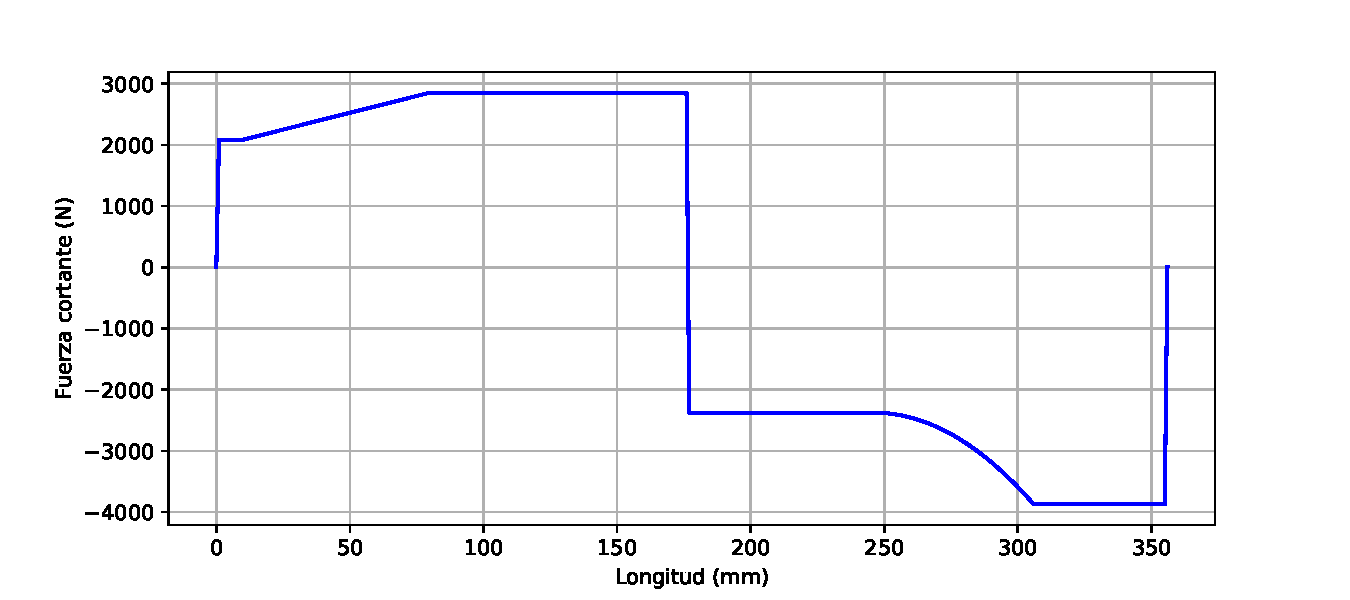
\includegraphics[scale=0.72]{Fuerzacortante.pdf}
\caption{Fuerza cortante}
\end{figure}
\chapter*{Momento flector}
$$
M = R_{1} <x>^{1} - \frac{12-n}{2}<x-10>^{2} + \frac{12-n}{2}<x-80>^{2} - (5000+10n)<x-(130+2n)>^{1} +$$
$$(60000+200n)<x-(130+2n)>^{0} - \frac{5/6}{6}<x-(200+2n)>^{3} + \frac{50}{2}<x-(260+2n)>^{2} + $$
$$ \frac{5/6}{6}<x-(260+2n)>^{3} + R_{2}<x-(310+2n)>^{1}
$$
De la misma forma, hallamos los valores para el momento flector
\begin{pyglist}[language=python,caption={Cálculo del momento flector},style=tango]
m = []
for x in range(0,310+2*n+1):
    aux = R1*x
    if x>10:
        aux = aux-(12-n)*(x-10)*(x-10)/2
    if x>130+2*n:
        aux = aux-(5000+10*n)*(x-(130+2*n))
    if x>80:
        aux = aux + (12-n)*(x-80)*(x-80)/2
    if x>260+2*n:
        aux = aux+(25)*(x-(260+2*n))**2 + (5/36)*(x-(260+2*n))**3
    if x > 130+2*n:
        aux = aux+(60000+200*n)
    if x>200+2*n:
        aux = aux-(5/36)*(x - (200+2*n))*(x - (200+2*n))*(x - (200+2*n))
    if x>=310+2*n:
        aux = aux + R2*(x-(310+2*n))
    m.append(aux)
plt.figure(figsize=(10,5))
plt.grid()
plt.xlabel('Longitud (mm)')
plt.ylabel('Momento flector (N-mm)')
plt.plot(m)
plt.savefig('momento.pdf')
\end{pyglist}
\begin{figure}[H]
\centering
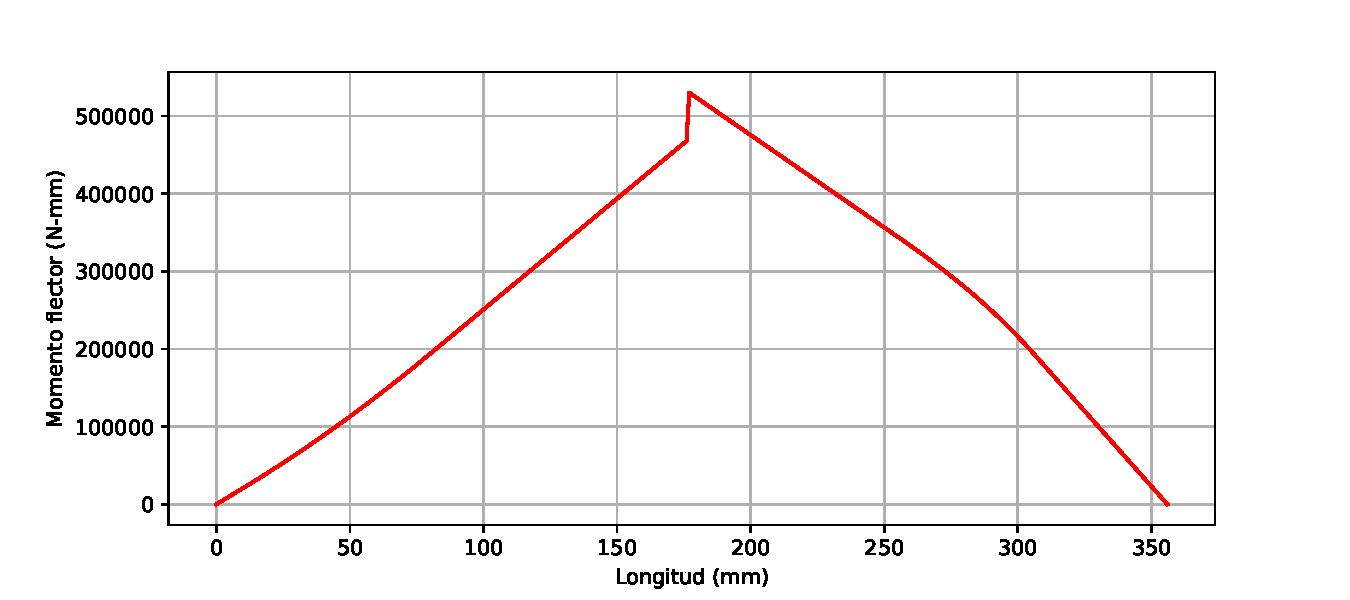
\includegraphics[scale=0.72]{momento.pdf}
\caption{Momento flector}
\end{figure}
\chapter*{Momento de inercia}
\begin{pyglist}[language=python,caption={Cálculo del momento flector},style=tango]
I = []
for i in range(0,310+2*n+1):
    if i<10:
        I.append((math.pi*(40)**4)/64)
        continue
    if i<80:
        I.append((math.pi*(50)**4)/64)
        continue
    if i<200+2*n:
        I.append((math.pi*(((50+((i-80)*20/(120+2*n))))**4)/64))
        continue
    if i<260+2*n:
        I.append((math.pi*(70)**4)/64)
        continue
    if i<300+2*n:
        I.append((math.pi*(60)**4)/64)
        continue
    I.append((math.pi*(55)**4)/64)
plt.figure(figsize=(15,5))
plt.grid()
plt.xlabel('Longitud (mm)')
plt.ylabel('Momento de inercia (mm$^4$)')
plt.plot(I,'-m')
plt.savefig('momentoi.pdf')
\end{pyglist}
\begin{figure}[H]
\centering
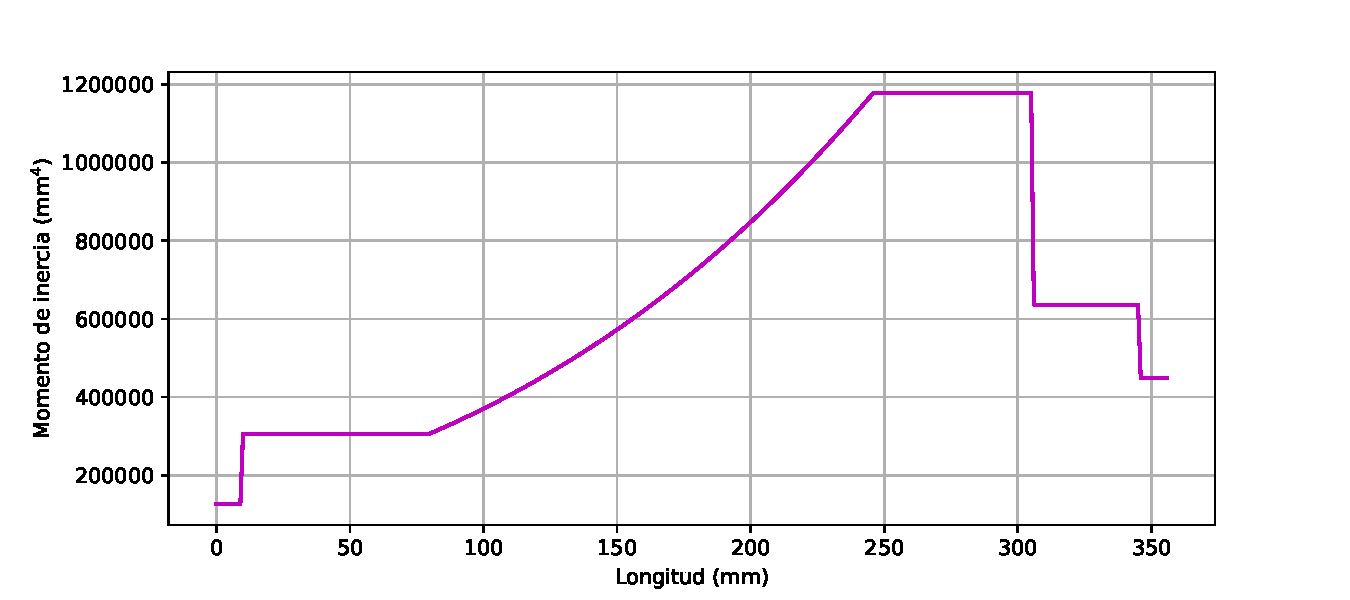
\includegraphics[scale=0.72]{momentoi.pdf}
\caption{Momento de inercia}
\end{figure}
\begin{pyglist}[language=python,caption={Cálculo del momento flector},style=tango]
E = 2.1*10**5
MEI = []
for i in range(0,310+2*n+1):
    MEI.append(m[i]/(E*I[i]))
plt.figure(figsize=(15,5))
plt.grid()
plt.xlabel('Longitud (mm)')
plt.ylabel('M/EI (mm)')
plt.plot(MEI,'-b')
plt.savefig('mei.pdf')
\end{pyglist}
\begin{figure}[H]
\centering
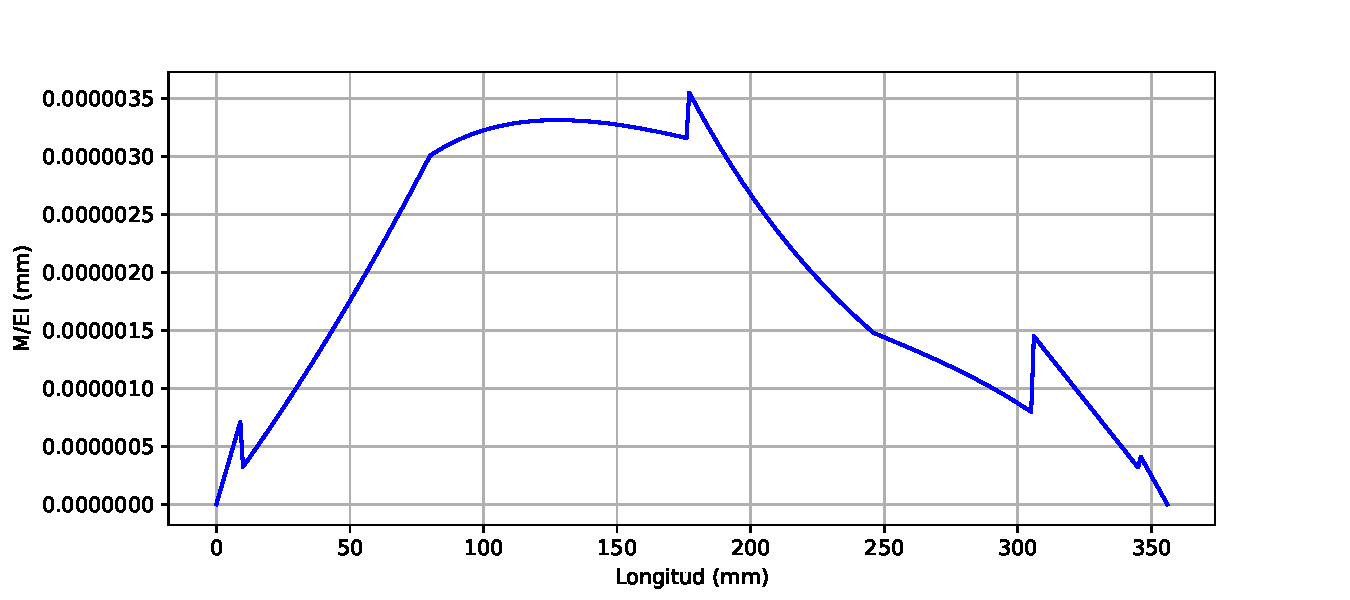
\includegraphics[scale=0.72]{mei.pdf}
\caption{M/EI}
\end{figure}
\chapter*{Cálculo de la deflexión}
Teniendo los valores de M, entonces pasamos I dividiendo e integramos:
$$
\int M/I\,\mathrm{d}x = ??
$$
Sabemos sin embargo, que si la función $M/I$ es continua e integrable, entonces podemos hallar su integral definida:
$$
\int_{0}^{310+2n} M/I\,\mathrm{d}x = \left[ \int M/I\,\mathrm{d}x \right]_{310+2n} - 0
$$
Debido a que es complicado hallar la integral de $M/I$, optamos por hallar la integral definida para cada punto entre 0 y 310+2n de manera numérica, la cual es fácil de hallar. Recordando que los valores obtenidos corresponden a la de la integral $\int M/I \, \mathrm{d}x$
\begin{pyglist}[language=python,caption={Primera integral de M/I},style=tango]
mi = []
mi.append(0)
for i in range(1,310+2*n+1):
    mi.append(m[i]/I[i] + mi[i-1])
plt.figure(figsize=(10,5))
plt.xlabel('Longitud (mm)')
plt.ylabel('$\int M/I$ (N/mm$^{2}$)')
plt.grid()
plt.plot(mi)
plt.savefig('mintegr.pdf')
\end{pyglist}
\begin{figure}[H]
\centering
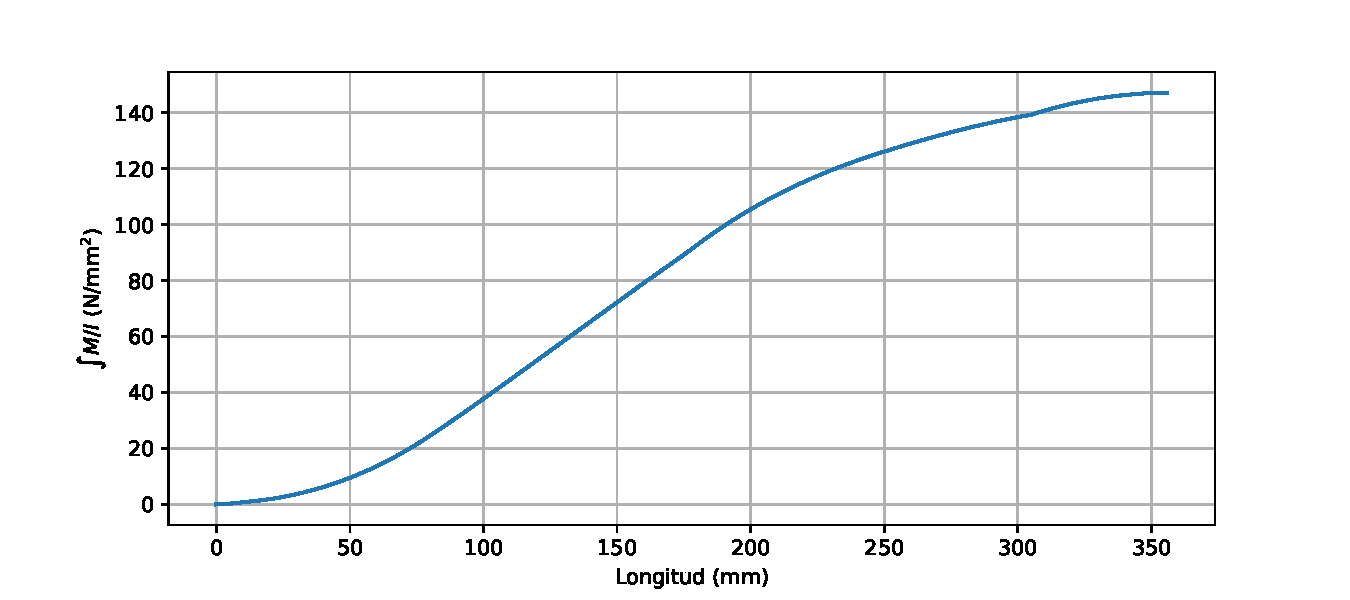
\includegraphics[scale=0.6]{mintegr.pdf}
\end{figure}
La gráfica obtenida corresponde cuando la constante de integración es 0.\\
Volvemos a integrar para hallar la deflexión del eje, de la misma forma, debido a que tenemos los valores de la primera integral de forma numérica. La gráfica resultante debe corresponde a
$$
\left[\iint M/I \,\mathrm{d}x\right]_{310+2n} 
$$
Con constante de integración 0 para las dos constantes.
\begin{pyglist}[language=python,caption={Segunda integral de M/I},style=tango]
mii = []
mii.append(0)
for i in range(1,310+2*n+1):
    mii.append(mi[i]+mi[i-1])
plt.figure(figsize=(10,5))
plt.grid()
plt.xlabel('Longitud (mm)')
plt.ylabel('$ \iint M/I\,\mathrm{d}x $ (MPa-mm)')
plt.plot(mii)
plt.savefig('m2i.pdf')
\end{pyglist}
\begin{figure}[H]
\centering
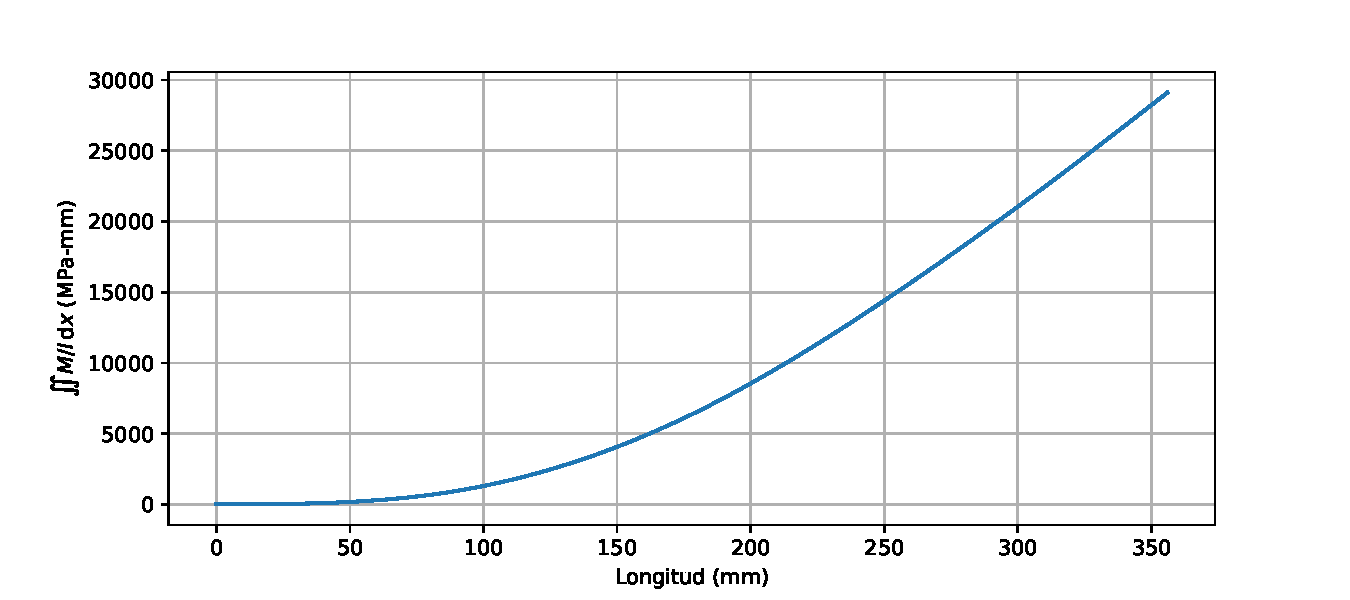
\includegraphics[scale=0.72]{m2i.pdf}
\end{figure}
\chapter{Deformada}
Para corregir el valor de las constantes de integración hallamos los valores que corresponden según las condiciones de frontera y dividimos entre E para hallar la deformada.
\begin{pyglist}[language=python,caption={Deformada},style=tango]
const = -mii[310+2*n]/(310+2*n)
for i in range(0,310+2*n+1):
    mii[i] = -(mii[i]+const*i)/E
plt.figure(figsize=(10,5))
plt.grid()
plt.xlabel('Longitud (mm)')
plt.ylabel('Deformada (mm)')
plt.plot(mii)
plt.savefig('def.pdf')
\end{pyglist}
\begin{figure}[H]
\centering
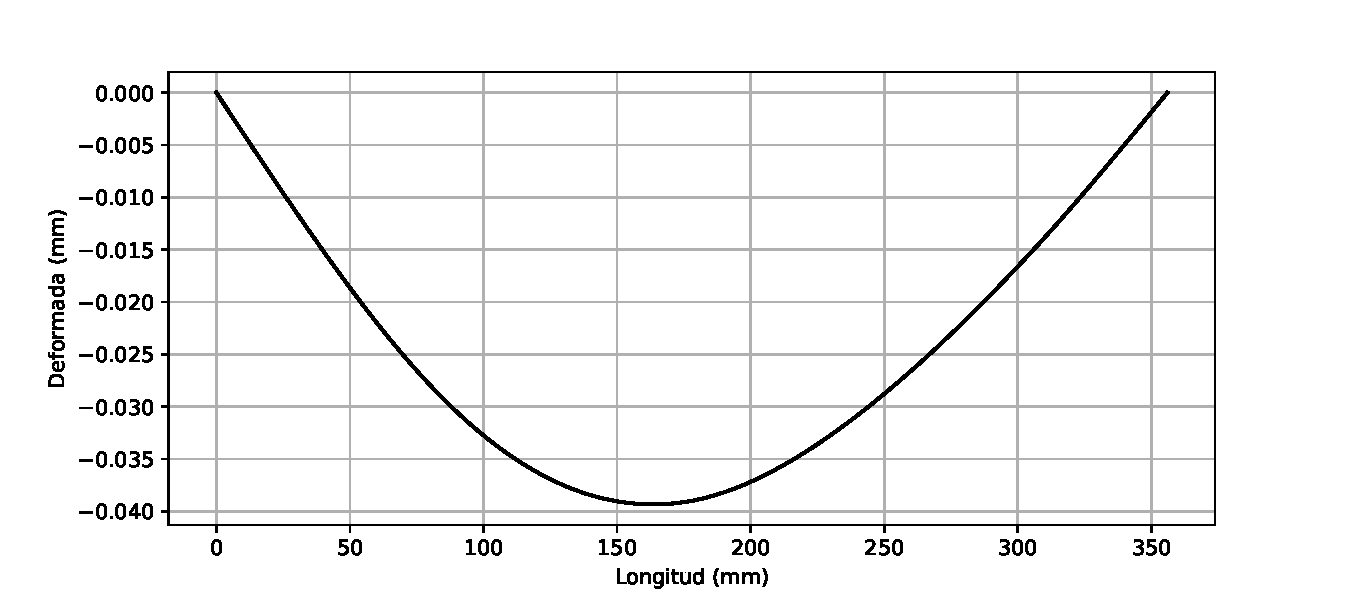
\includegraphics[scale=0.72]{def.pdf}
\caption{Gráfica de la deformada}
\end{figure}
\chapter{Flecha máxima}
\begin{pyglist}[language=python,caption={Cálculo de la flecha},style=tango]
flechamax = 0
posflecha = 0
for i in range(0,310+2*n+1):
    flechamax = max(flechamax,abs(mii[i]))
for i in range(0,310+2*n+1):
    if(abs(mii[i]) == flechamax):
        posflecha = i
print(flechamax, posflecha)
\end{pyglist}
Obtenemos que el máximo valor de la flecha es \fbox{0.03934077\,mm} y sucede a \fbox{163\,mm} del extremo izquierdo.
\chapter{Ángulo formado por los extremos}
Realizamos una regresión lineal para hallar la ecuación que corresponde a una recta tangente al extremo izquierdo y el extremo derecho:
$$
\text{Ext. izquierdo}(x) = -4.0824\times 10^{-4}\,x - 2.4\times 10^{-7} \hspace{10pt} \text{Ext. derecho}(x) = 3.12\times 10^{-4}x - 1.1110683\times 10^{-1}
$$
Dado que las pendientes son muy pequeñas, se puede aproximar y considerar que $\tan (x) = x$:
$$
\theta = \pi /2 - (4.0824-3.12)\times 10^{-4} = 1.57070008 = \fbox{$89.9944858^{\circ}$}
$$
\begin{figure}[H]
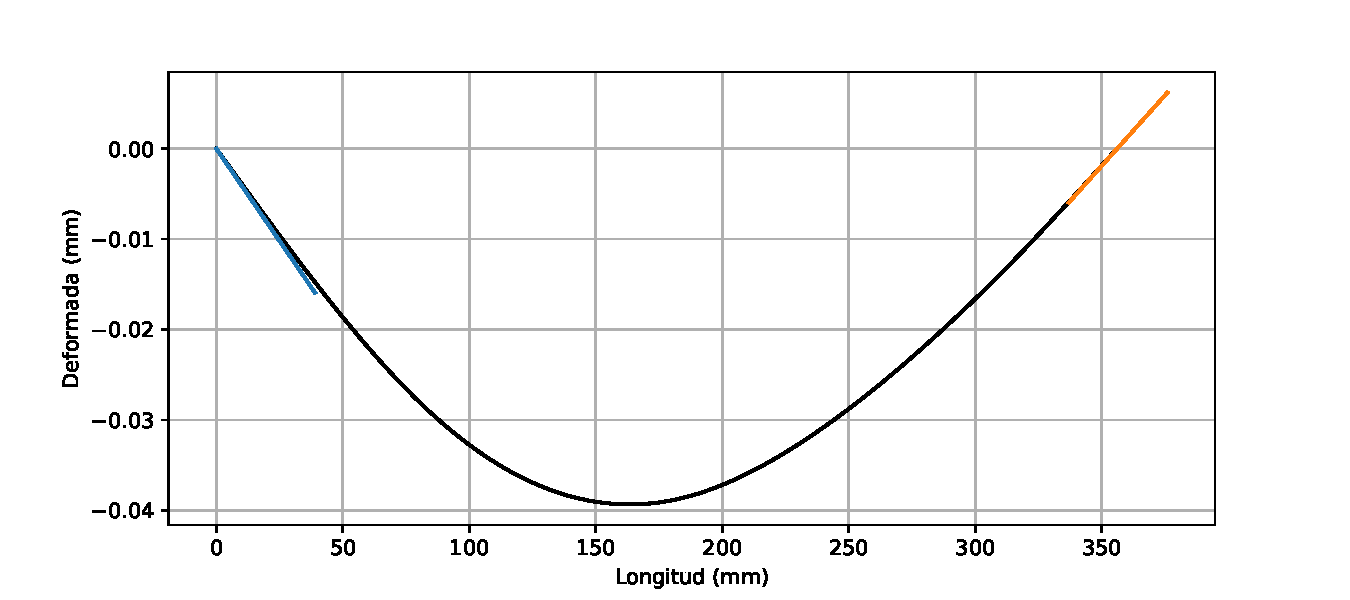
\includegraphics[scale=0.72]{ang.pdf}
\caption{Rectas tangentes}
\end{figure}
\chapter{Mayor esfuerzo}
\begin{pyglist}[language=python,caption={Cálculo del esfuerzo por flexión},style=tango]
esfm = 0
poses = 0
for i in range(0,310+2*n+1):
    if abs(math.sqrt(area[i]/math.pi)*m[i]/I[i]) > esfm:
        esfm = abs(math.sqrt(area[i]/math.pi)*m[i]/I[i])
        poses = i
print(esfm, poses)
\end{pyglist}
El esfuerzo máximo por flexión ocurre a 177\,mm del extremo izquierdo y es de 4.1418371\,MPa.
\begin{pyglist}[language=python,caption={Cálculo del esfuerzo máximo},style=tango]
esfm = 0
poses = 0
gresf = []
for i in range(0,310+2*n+1):
    esff = abs(math.sqrt(area[i]/math.pi)*m[i]/I[i])
    gresf.append(math.sqrt(esff**2 + (v[i]/area[i])**2))
    if math.sqrt(esff**2 + (v[i]/area[i])**2) > esfm:
        esfm = math.sqrt(esff**2 + (v[i]/area[i])**2)
        poses = i
print(esfm, poses)
plt.figure(figsize=(10,5))
plt.grid()
plt.xlabel('Longitud (mm)')
plt.ylabel('Esfuerzo (MPa)')
plt.plot(gresf)
plt.savefig('esfuerzo.pdf')
\end{pyglist}
El mayor esfuerzo, considerando la flexión y el de corte es de \fbox{44.852762\,MPa} y ocurre a \fbox{346\,mm.}
\begin{figure}[H]
\centering
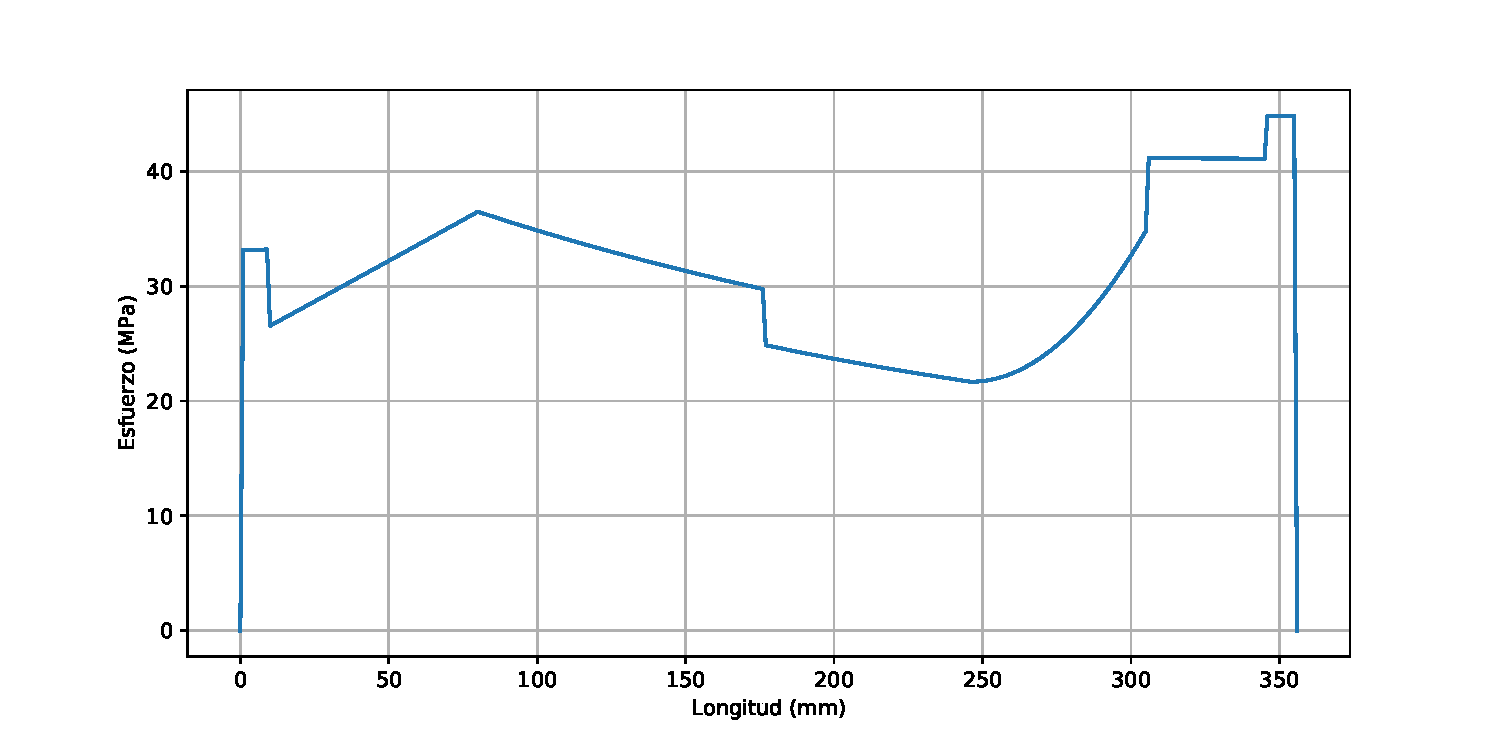
\includegraphics[scale=0.72]{esfuerzo.pdf}
\caption{Esfuerzo}
\end{figure}
\chapter{Anexos}
Como el problema ha sido programado según el valor de $n$. Podemos hallar el gráfico de la deformada para varios valores de $n$ de forma muy rápida, se anexa entonces varios gráficos de la deformada con distintos valores de $n$:
\begin{figure}[H]
\centering
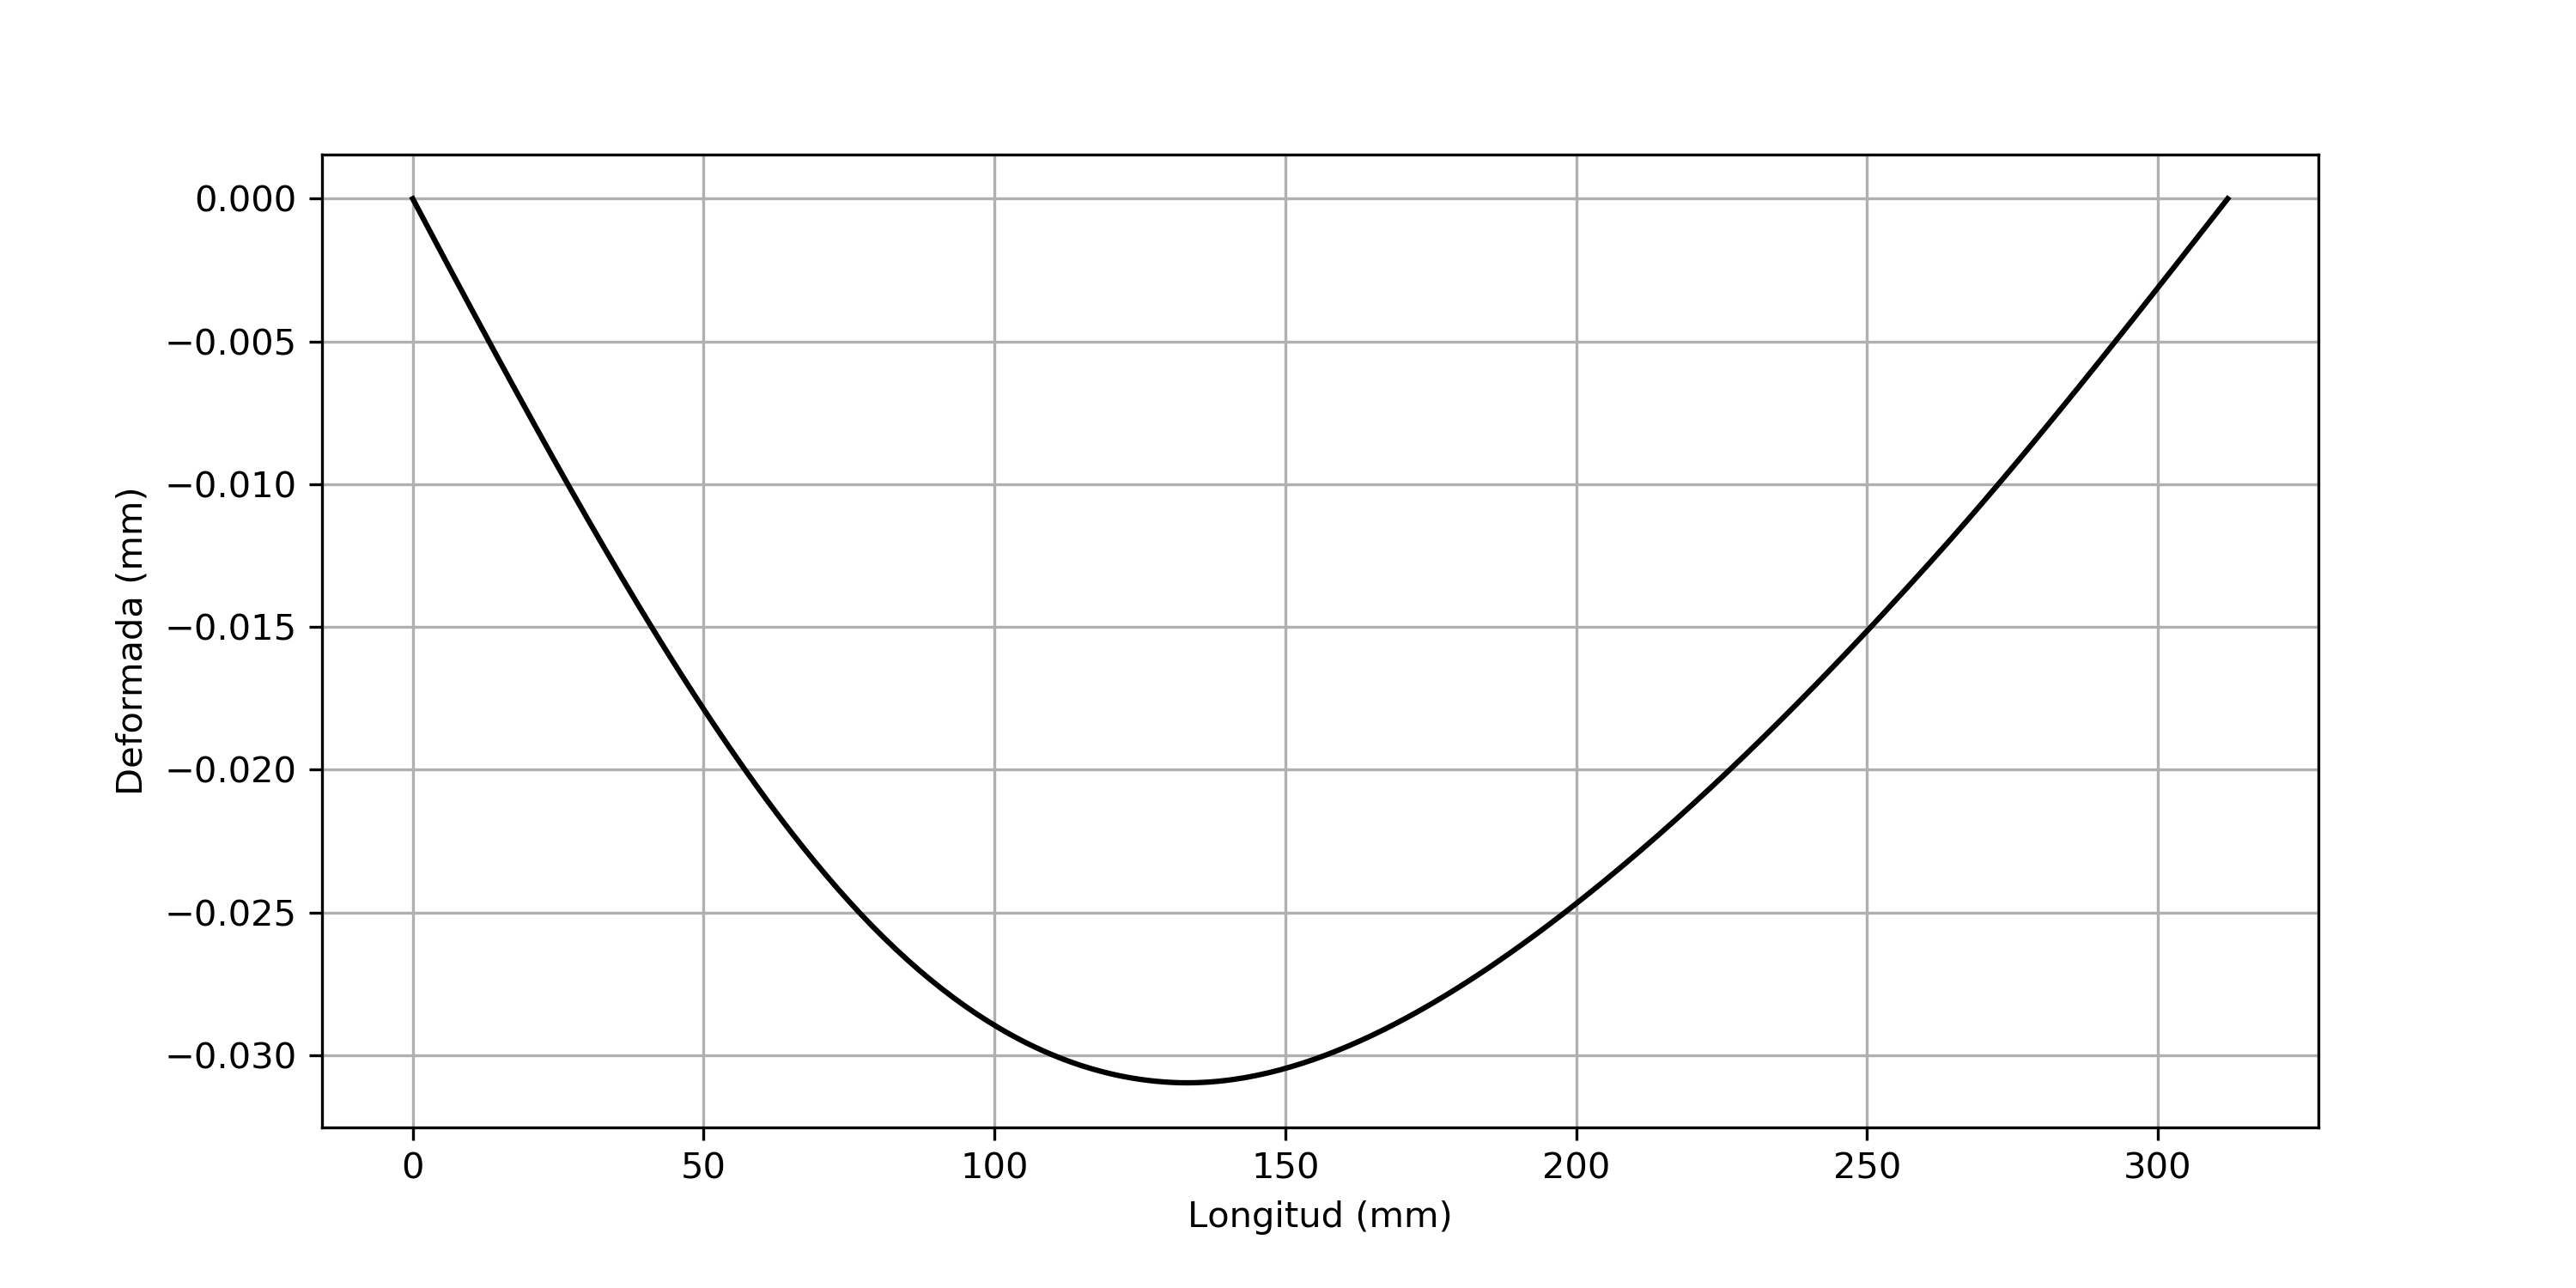
\includegraphics[scale=0.68]{defj1.png}
\caption{$n = 1$}
\end{figure}
\begin{figure}[H]
\centering
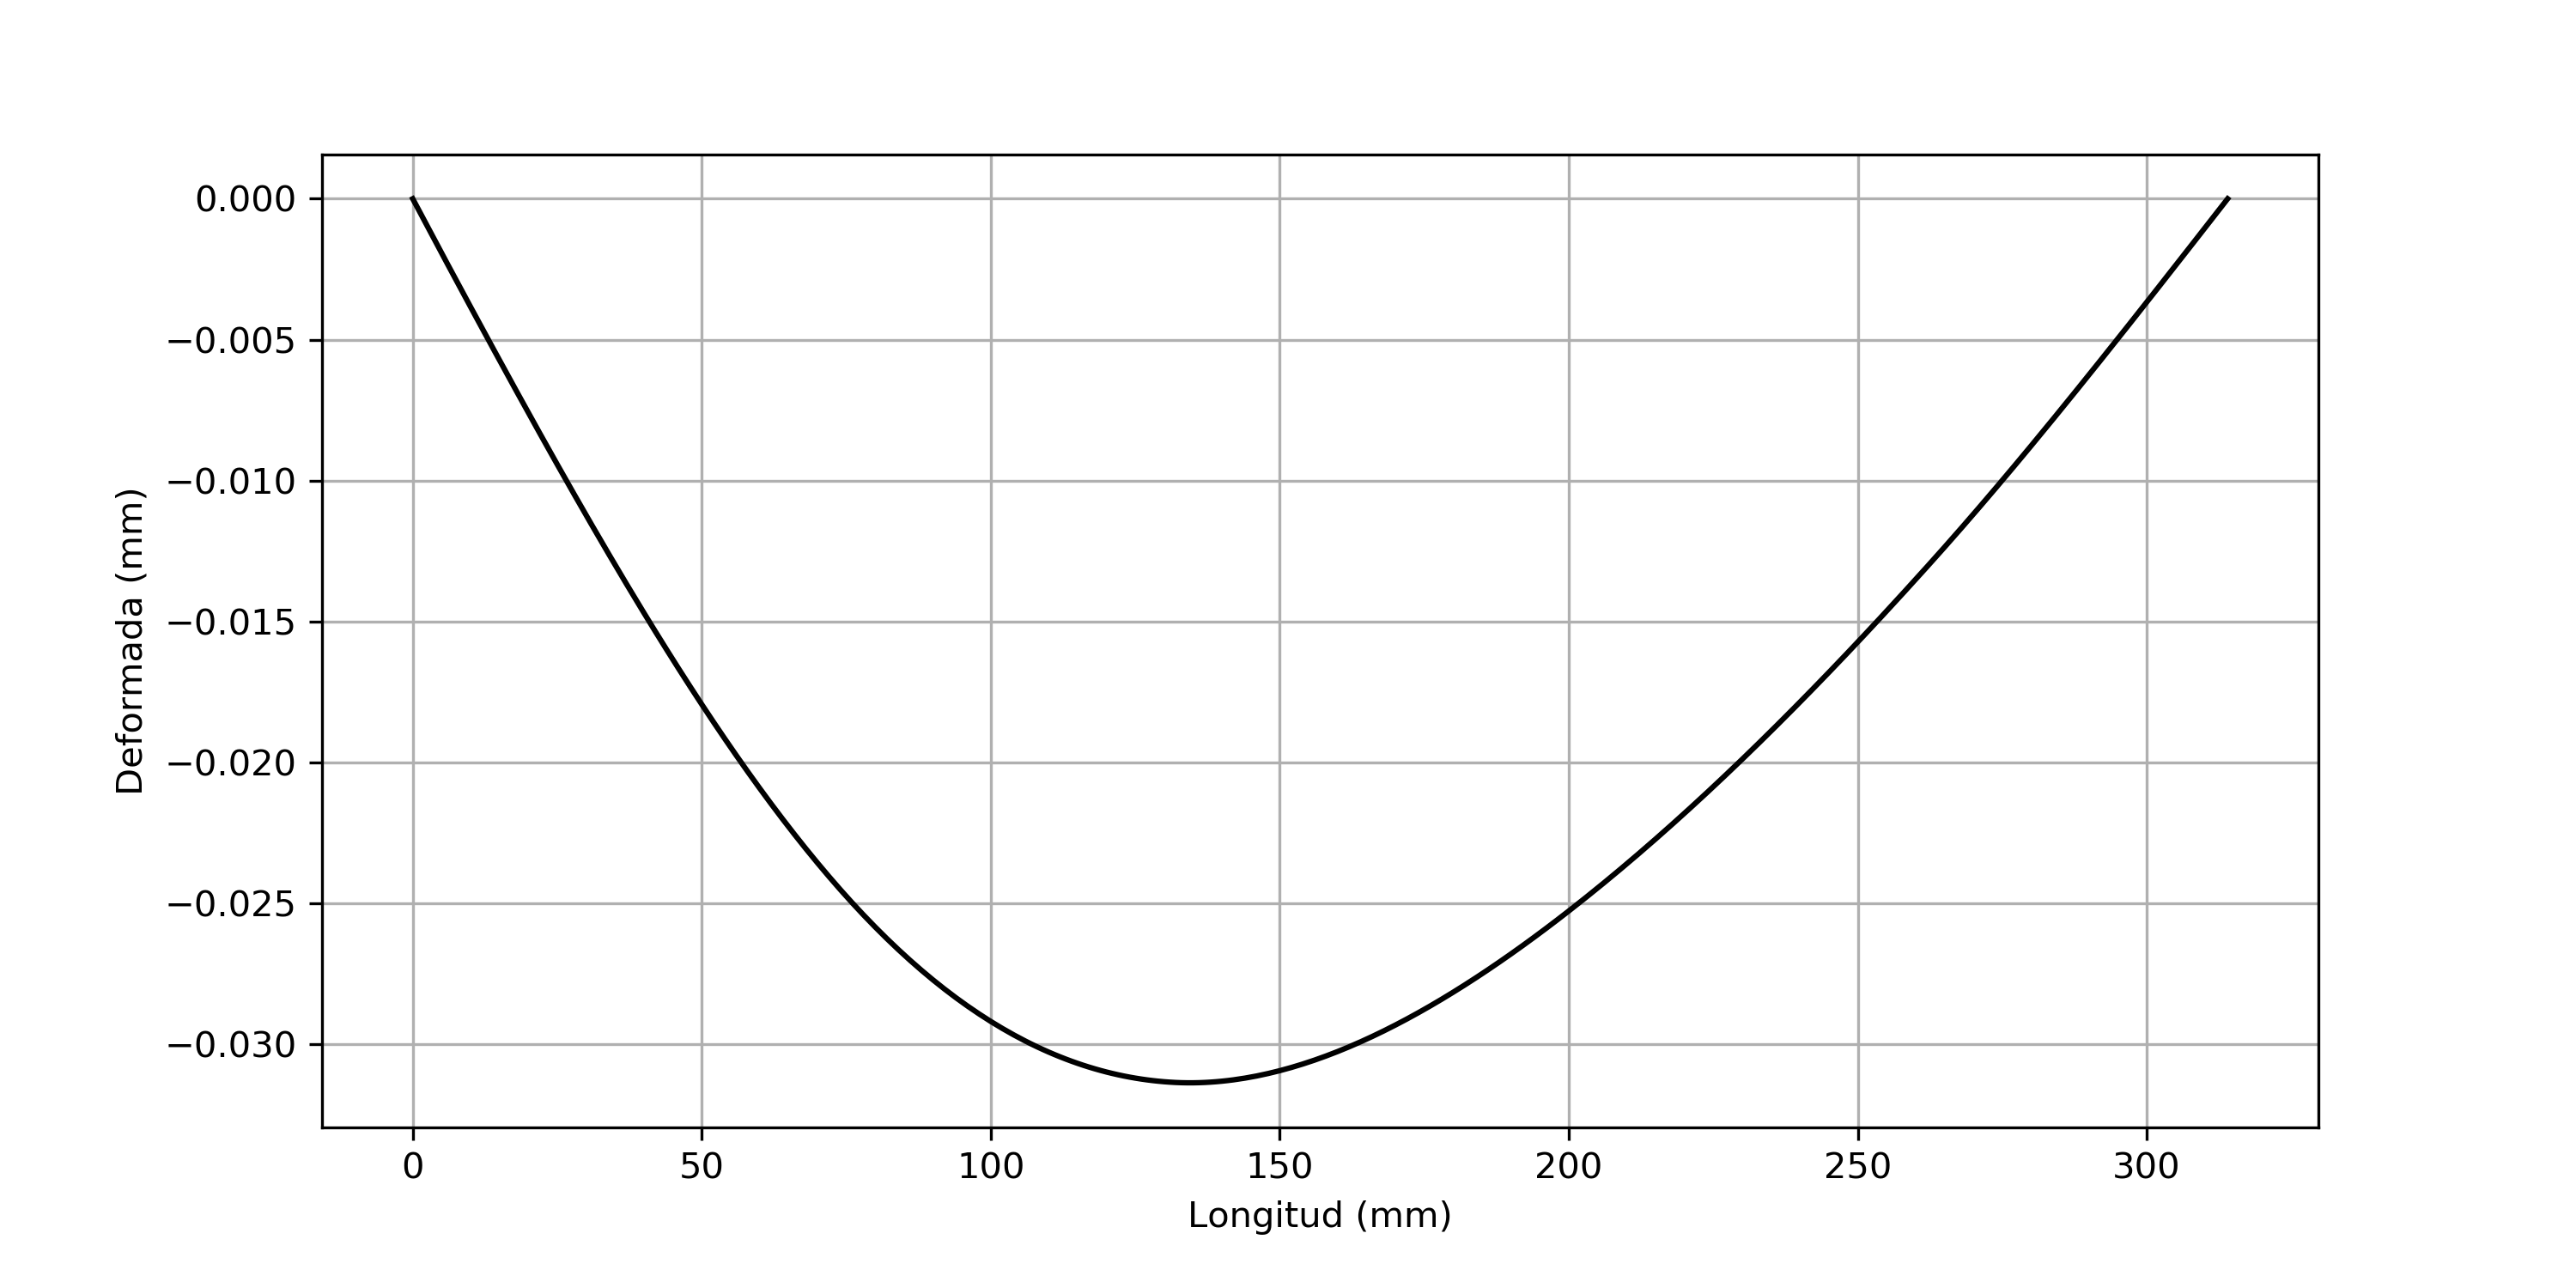
\includegraphics[scale=0.68]{defj2.png}
\caption{$n = 2$}
\end{figure}
\begin{figure}[H]
\centering
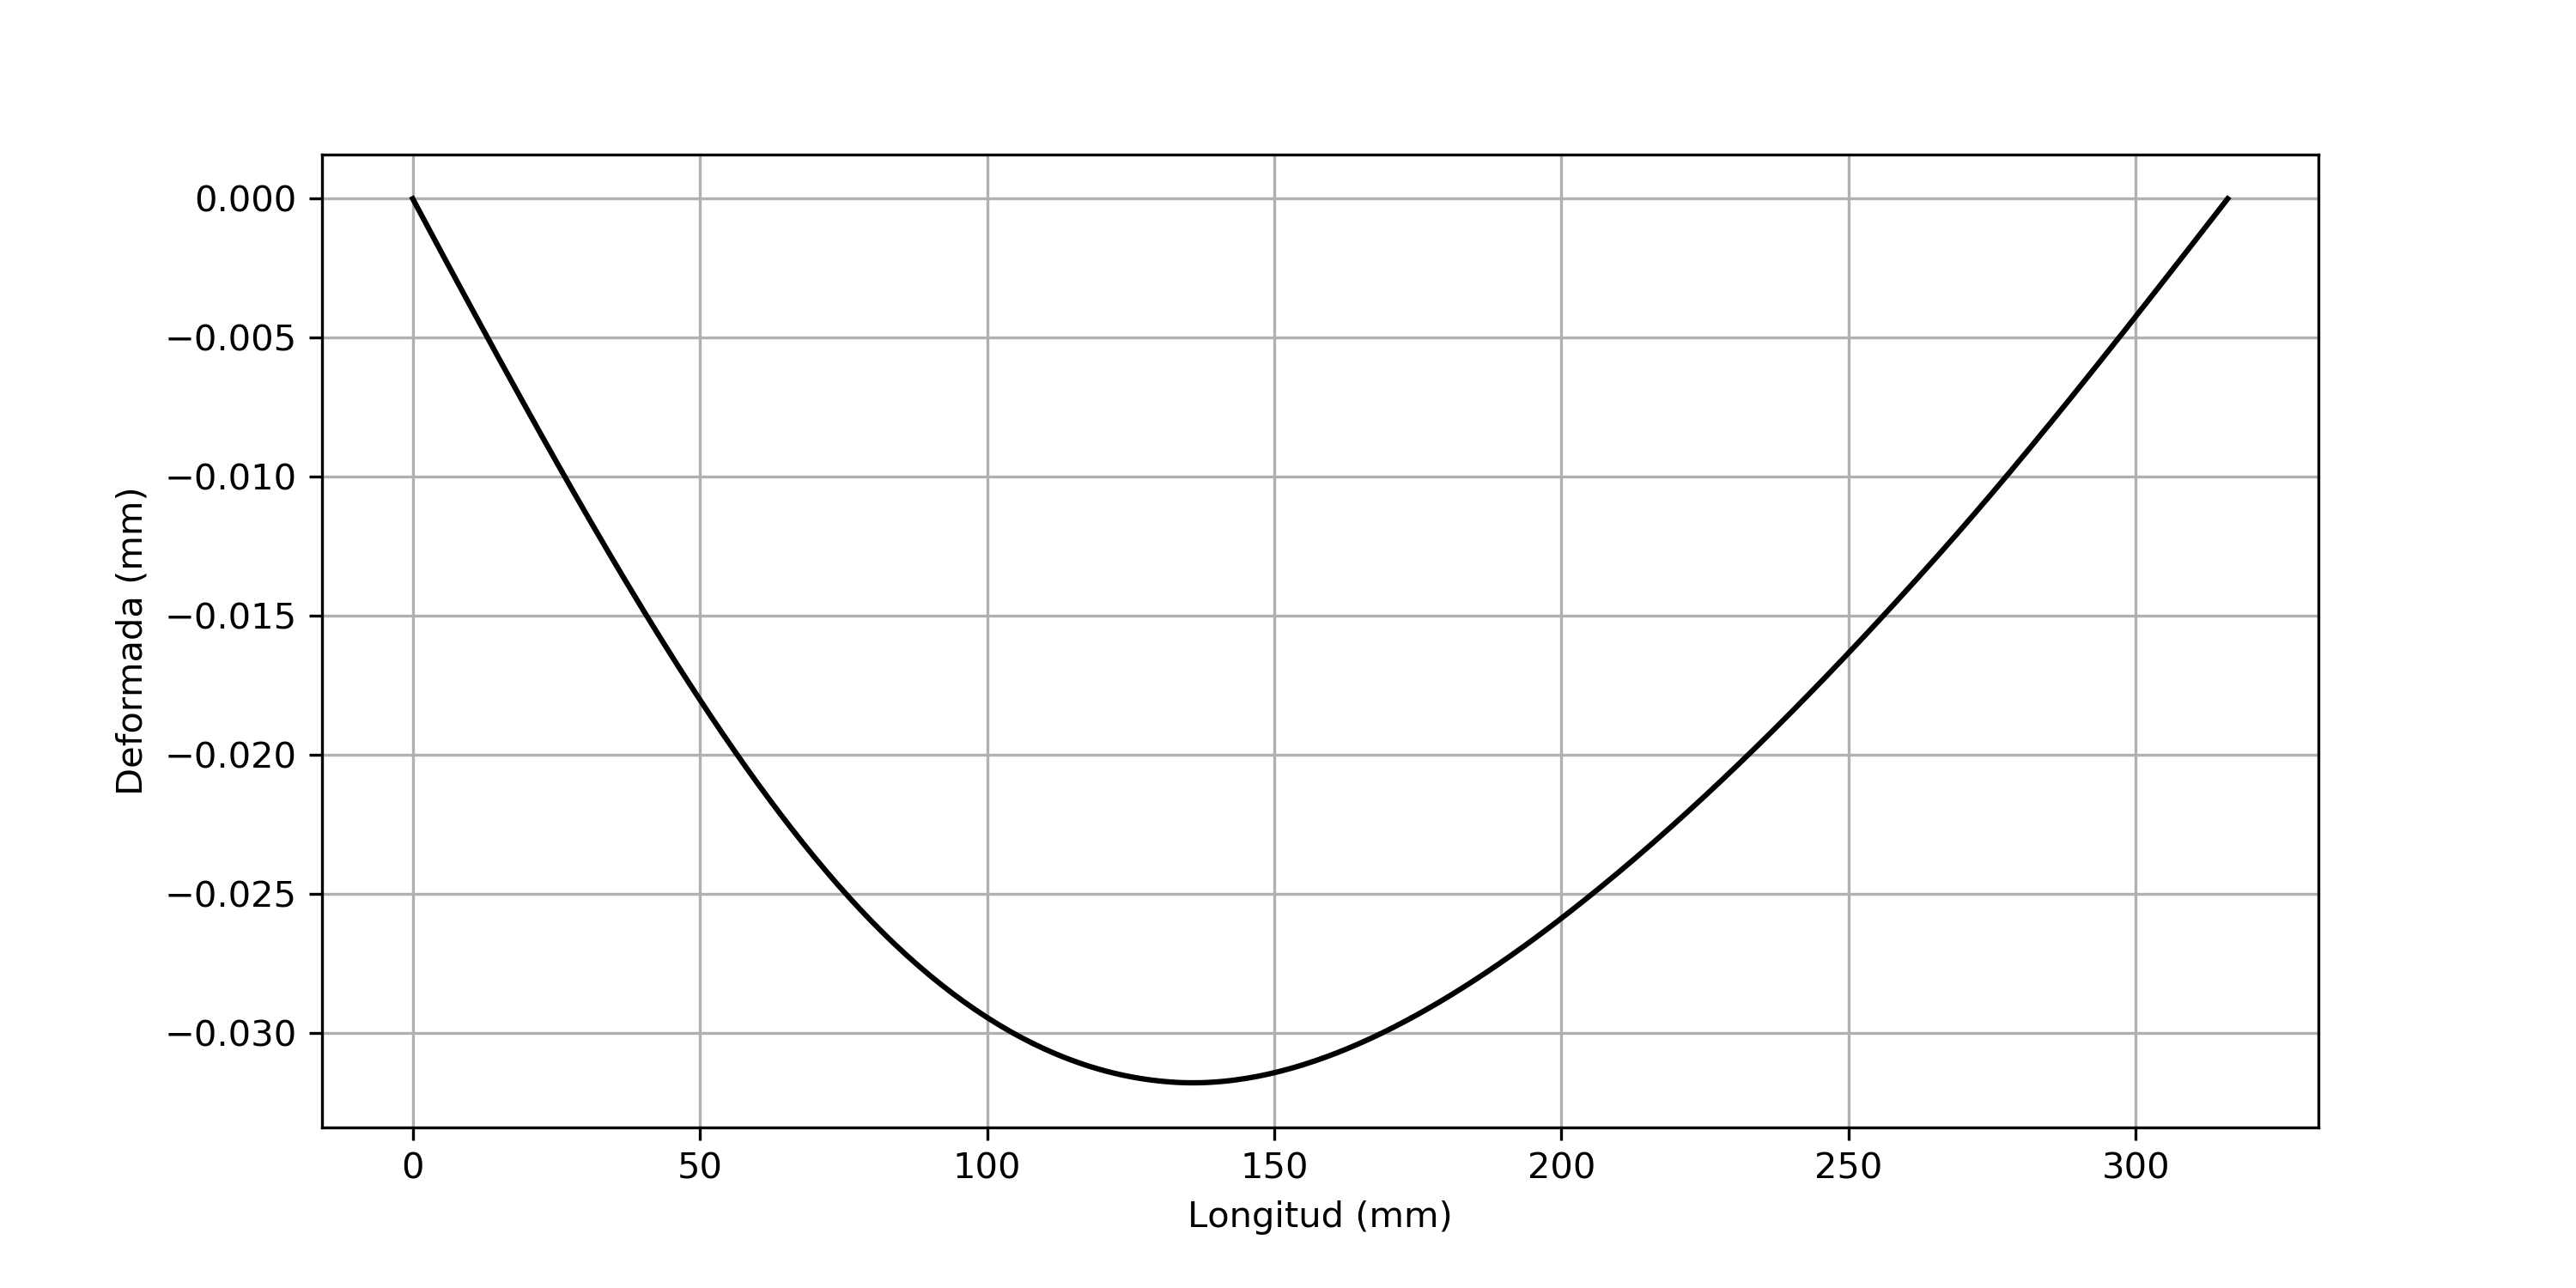
\includegraphics[scale=0.68]{defj3.png}
\caption{$n = 3$}
\end{figure}
\begin{figure}[H]
\centering
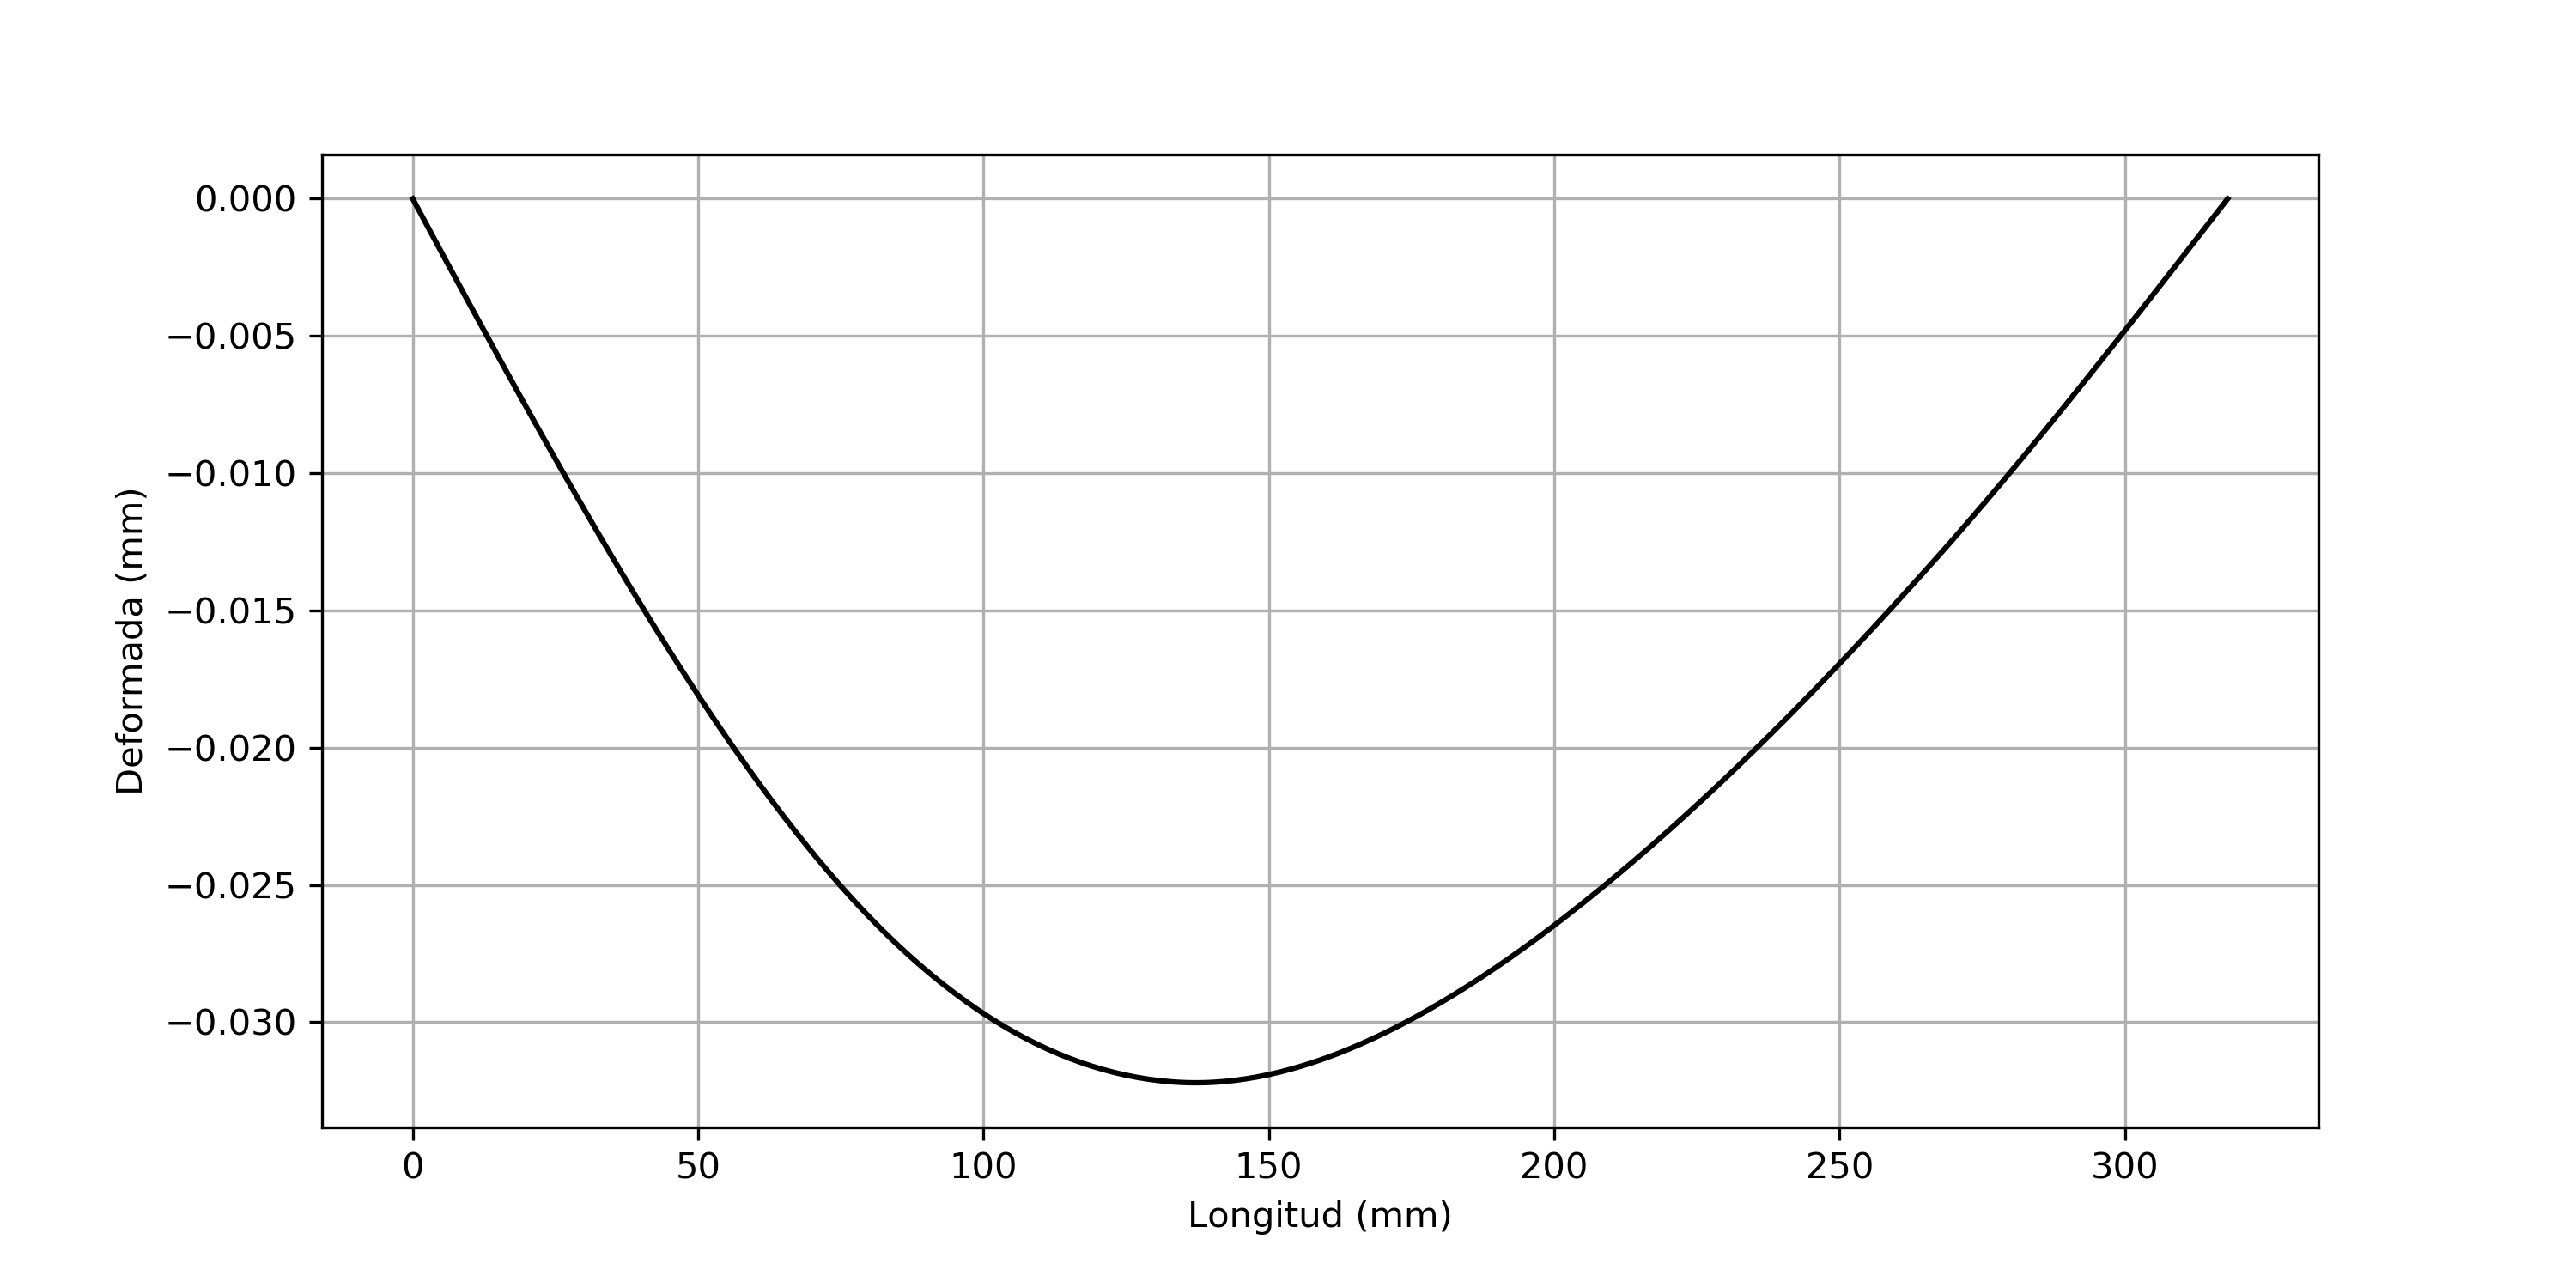
\includegraphics[scale=0.68]{defj4.png}
\caption{$n = 4$}
\end{figure}
\begin{figure}[H]
\centering
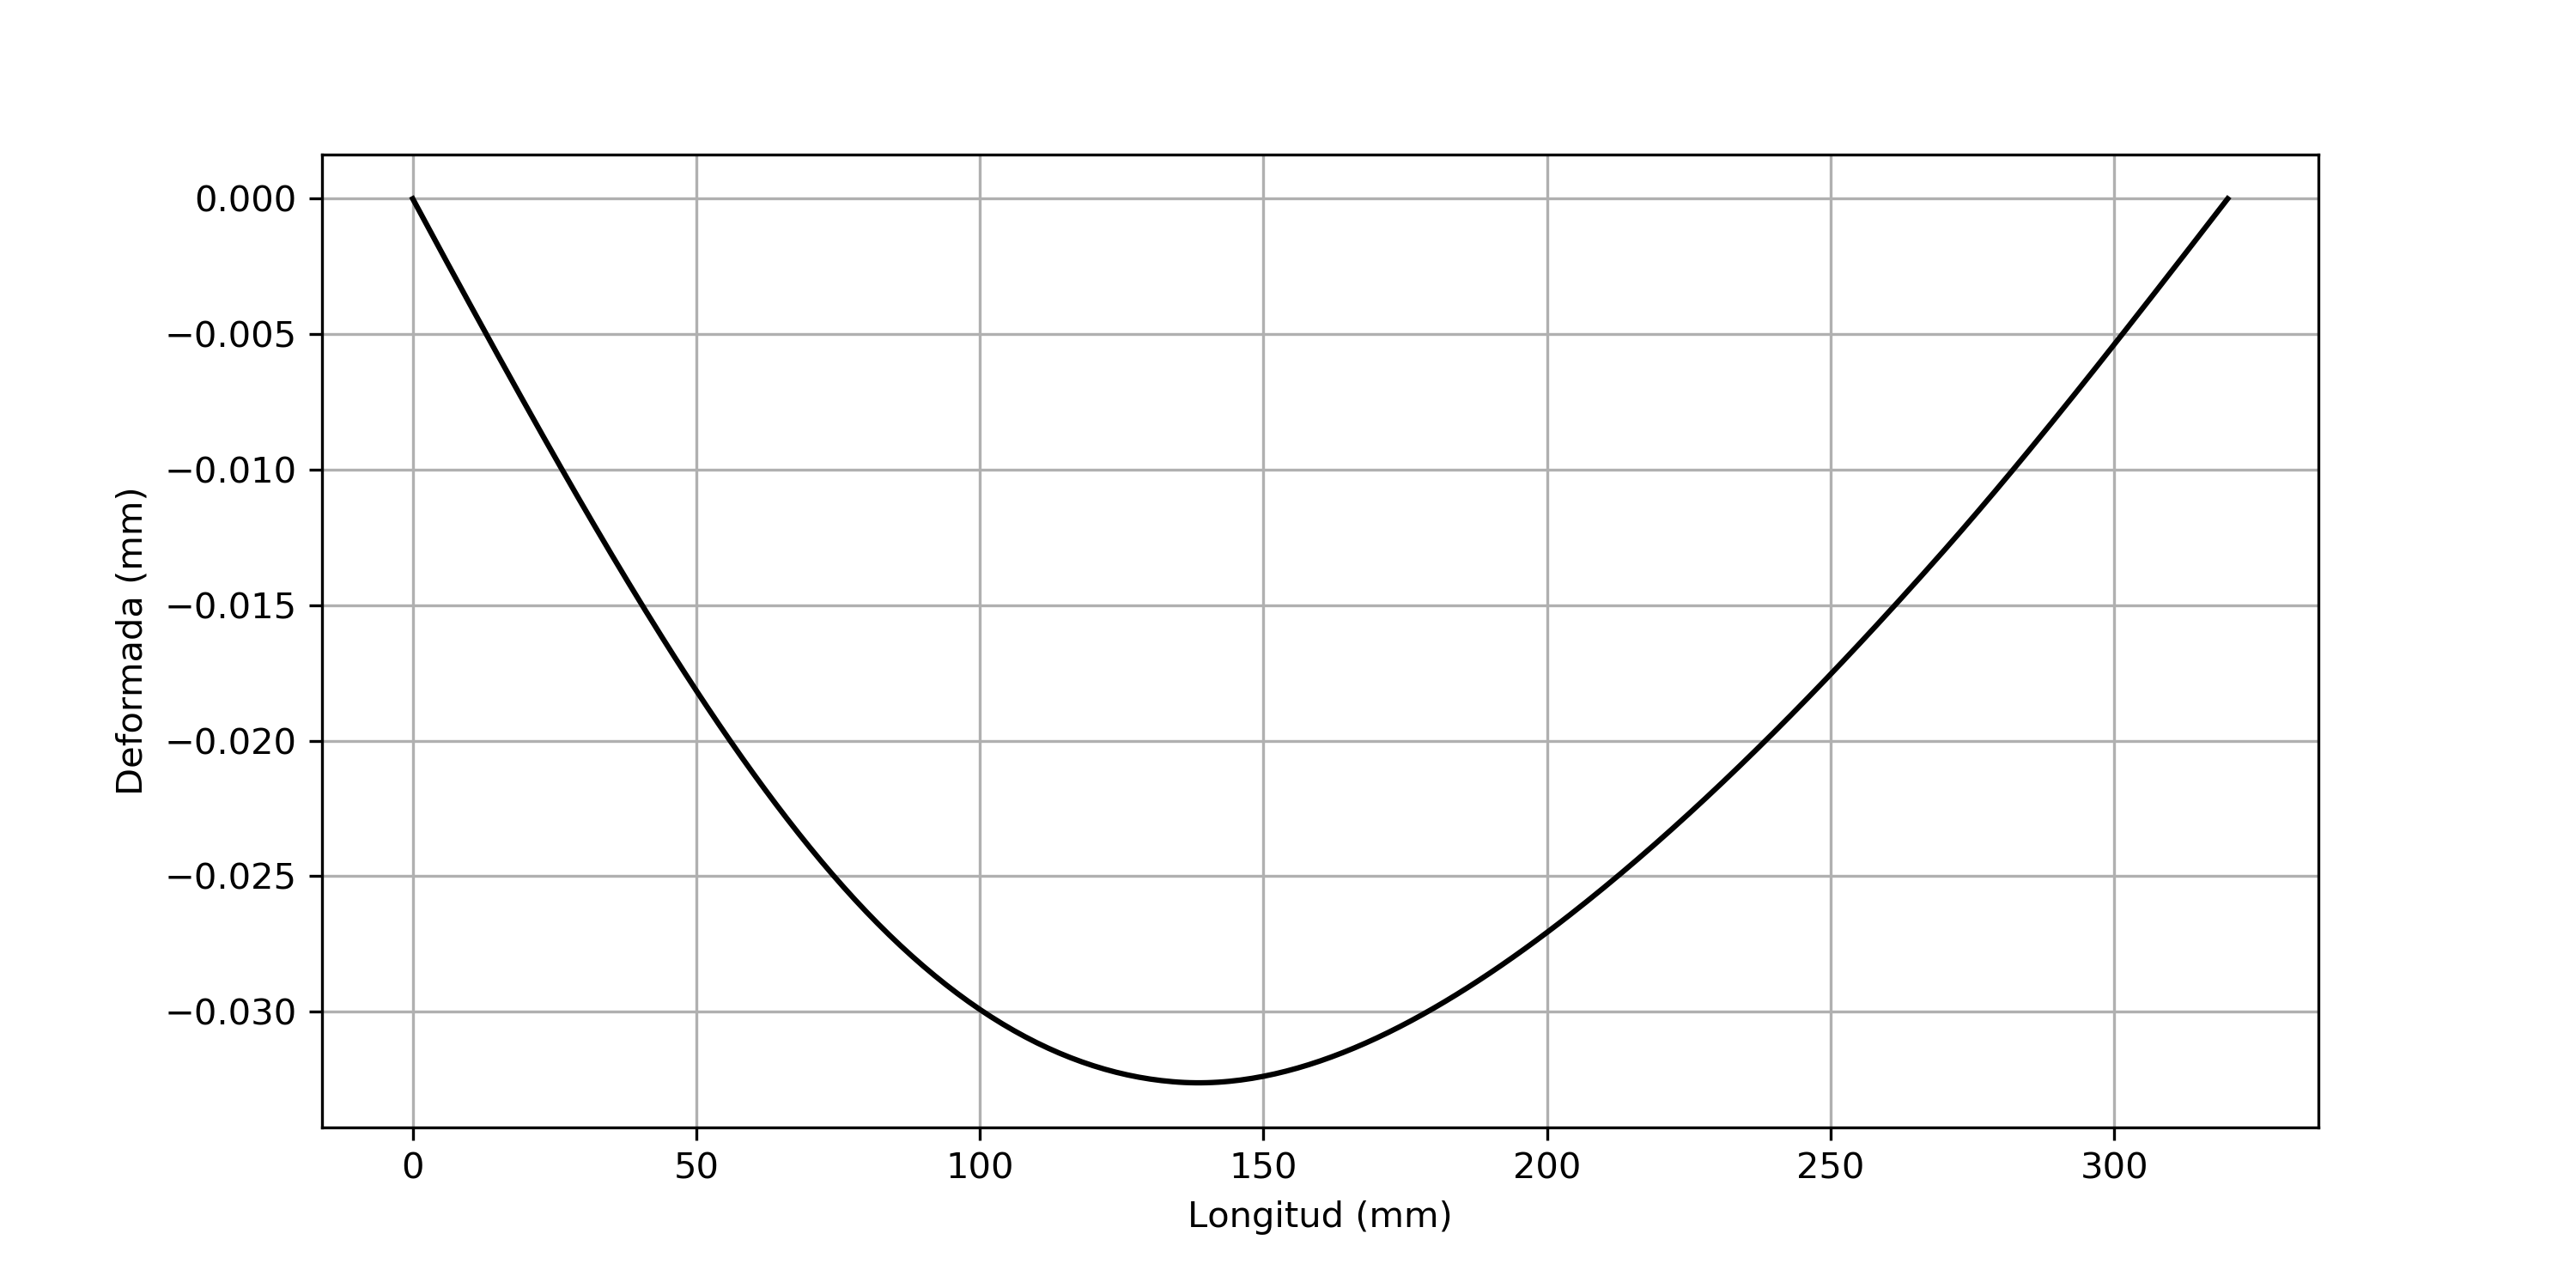
\includegraphics[scale=0.68]{defj5.png}
\caption{$n = 5$}
\end{figure}
\begin{figure}[H]
\centering
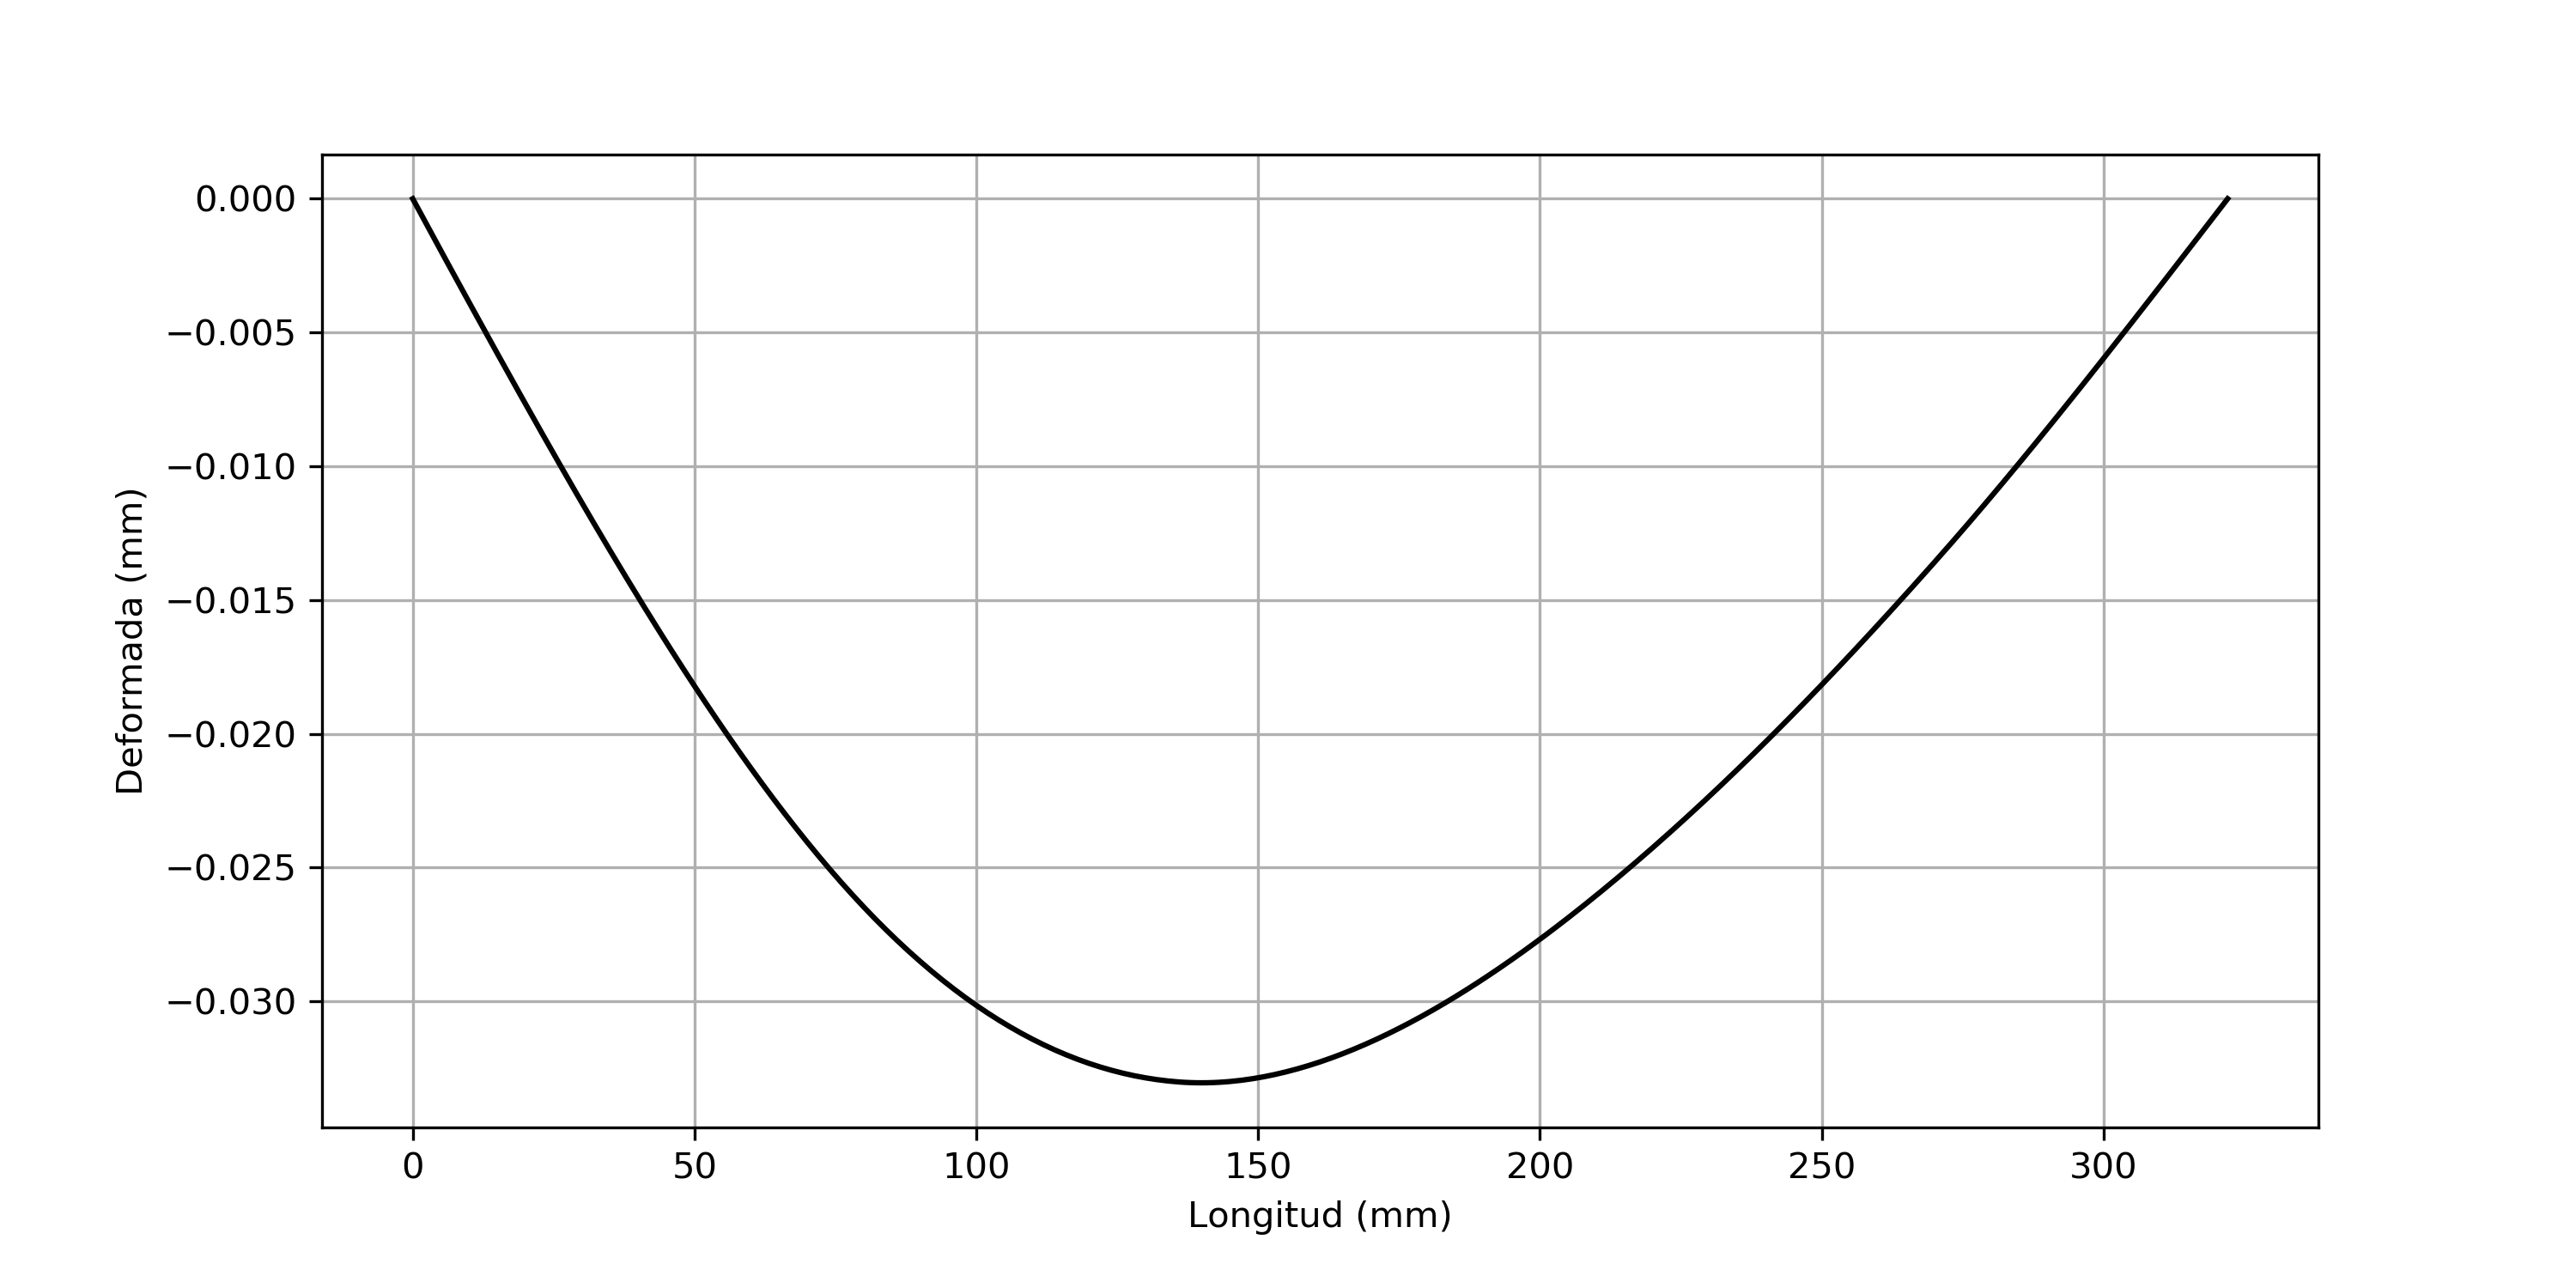
\includegraphics[scale=0.68]{defj6.png}
\caption{$n = 6$}
\end{figure}
\begin{figure}[H]
\centering
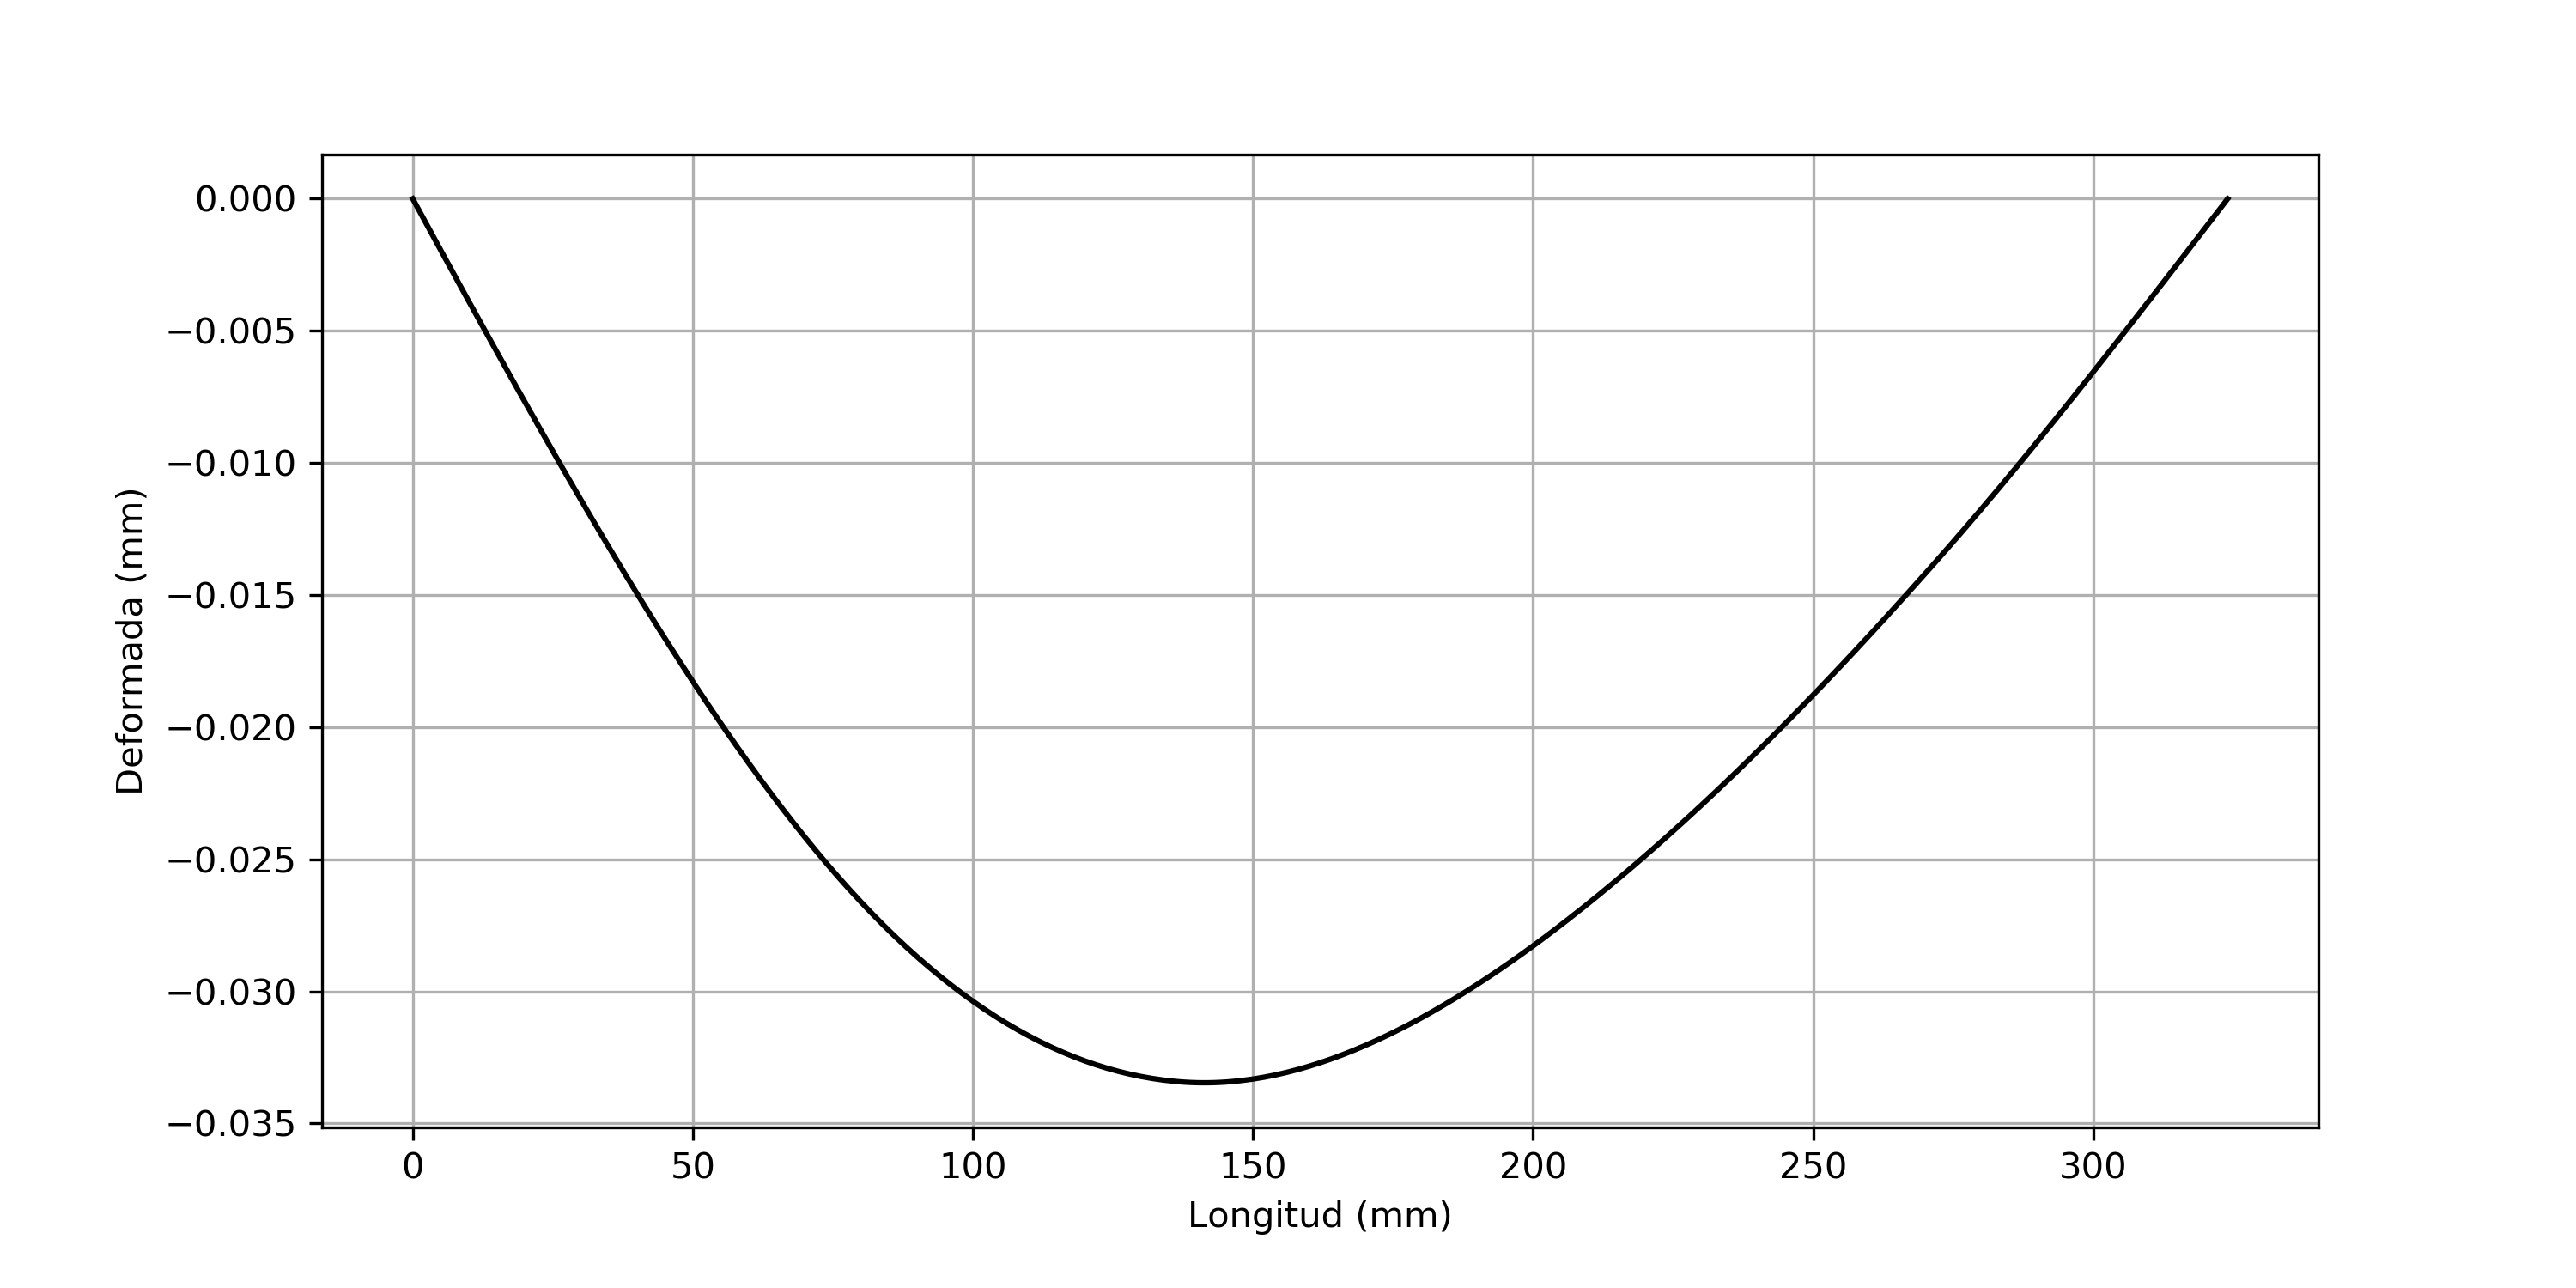
\includegraphics[scale=0.68]{defj7.png}
\caption{$n = 7$}
\end{figure}
\begin{figure}[H]
\centering
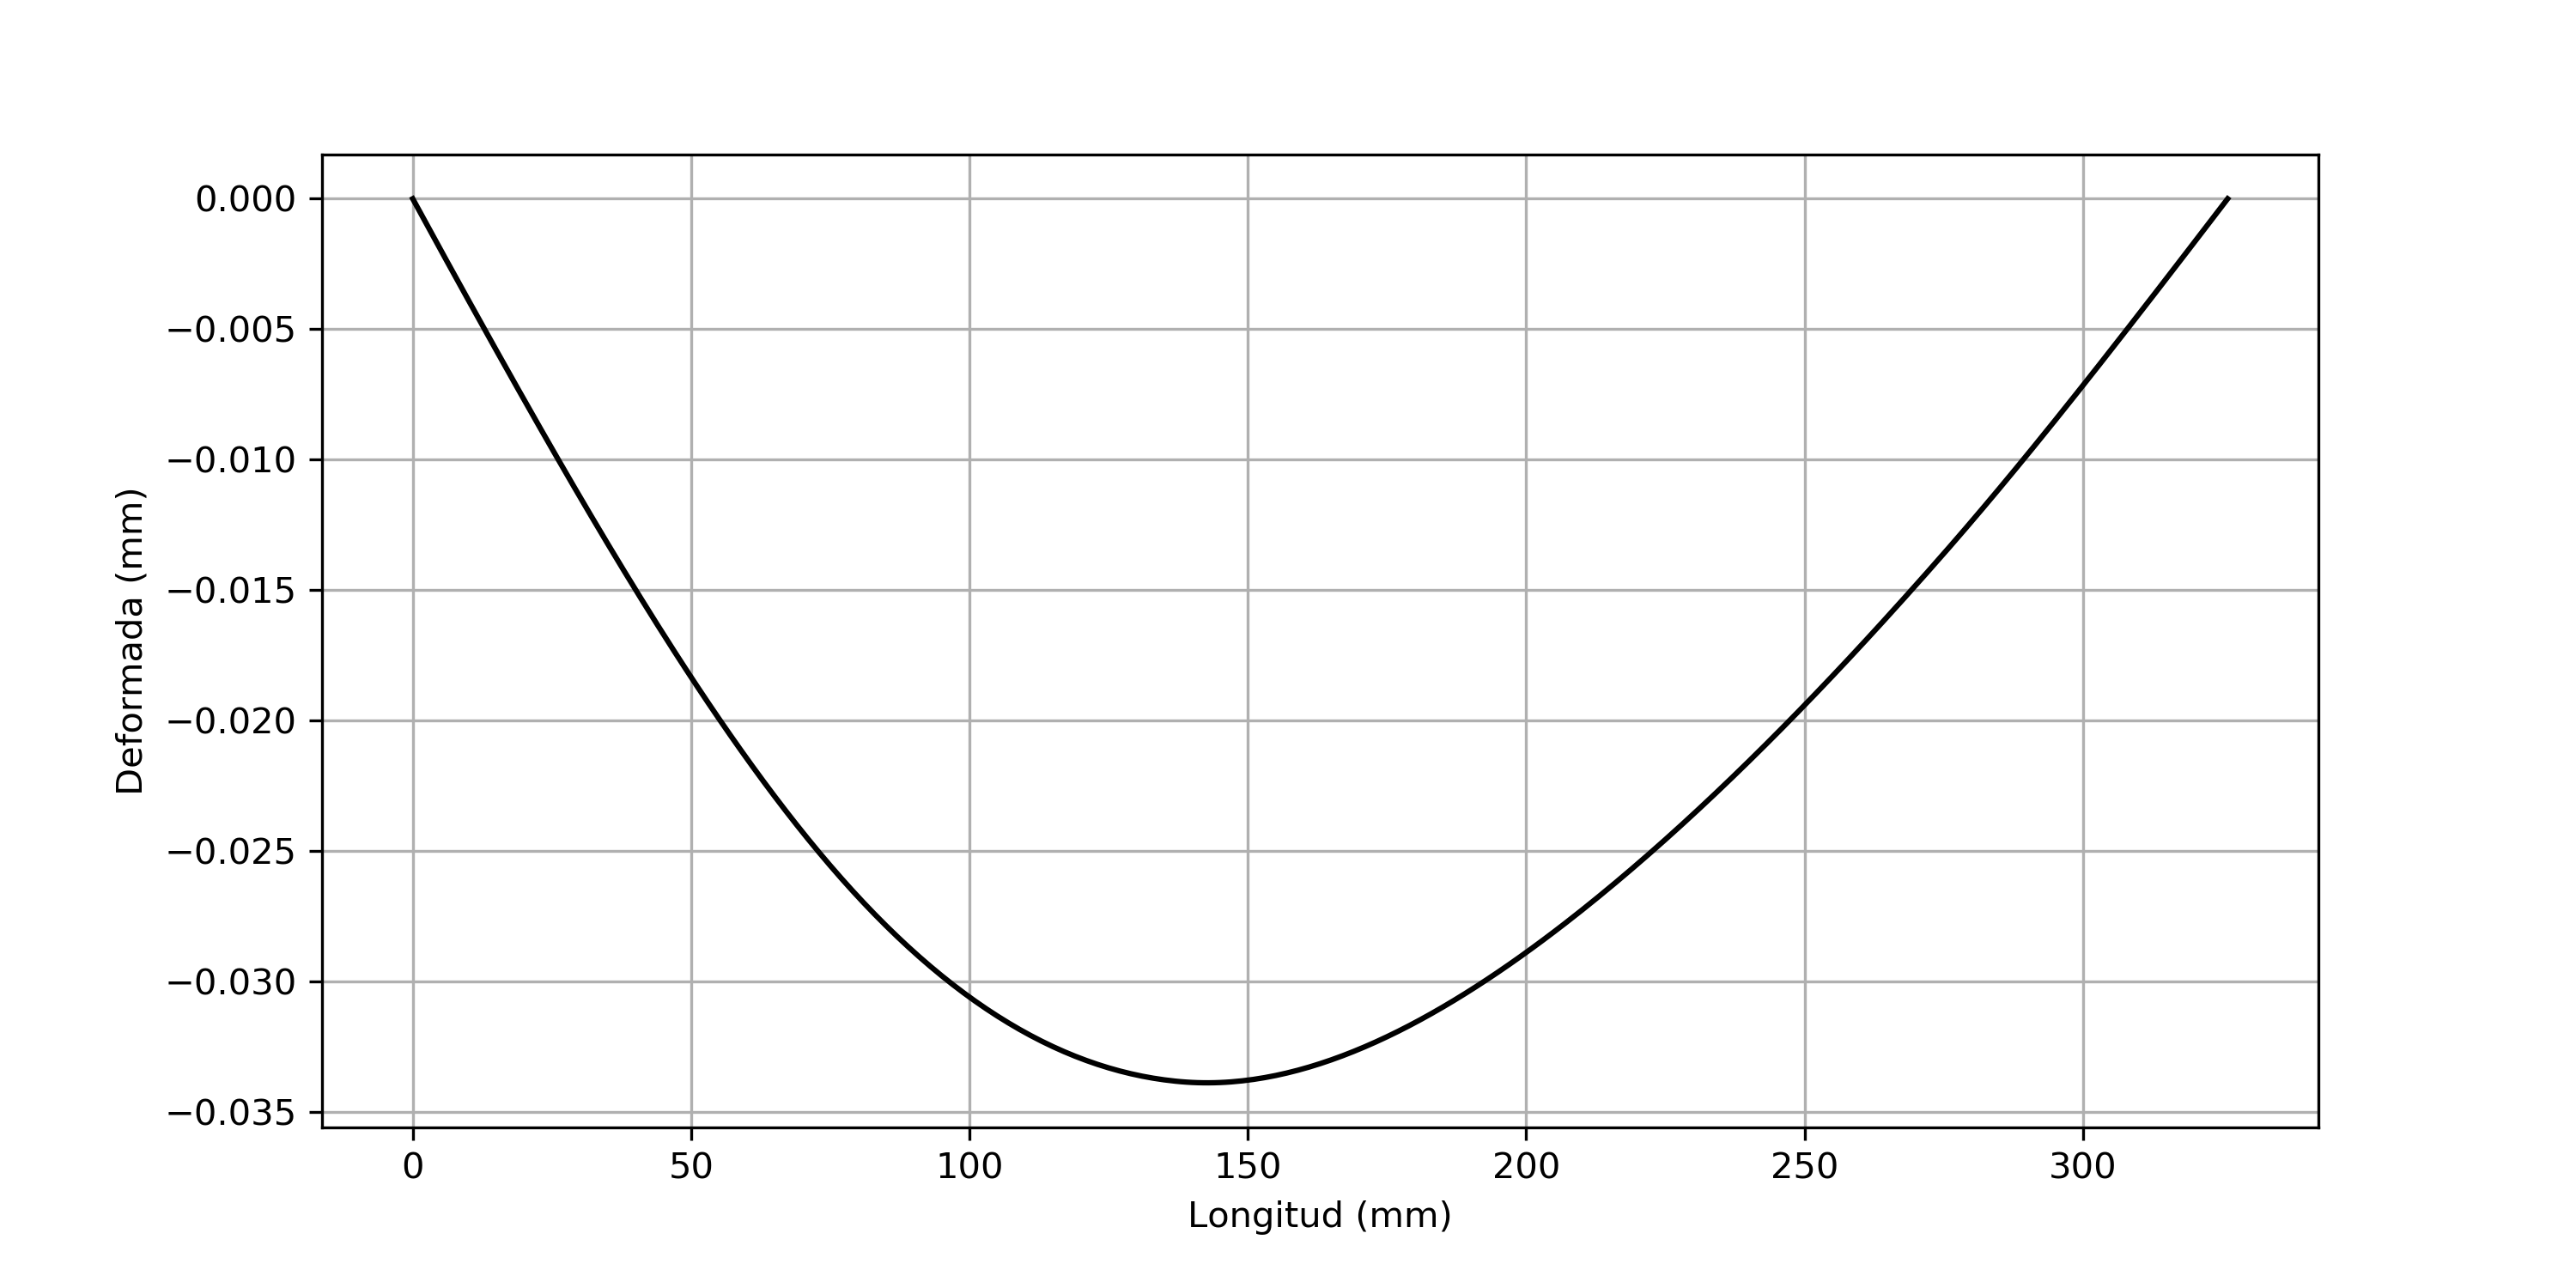
\includegraphics[scale=0.68]{defj8.png}
\caption{$n = 8$}
\end{figure}
\begin{figure}[H]
\centering
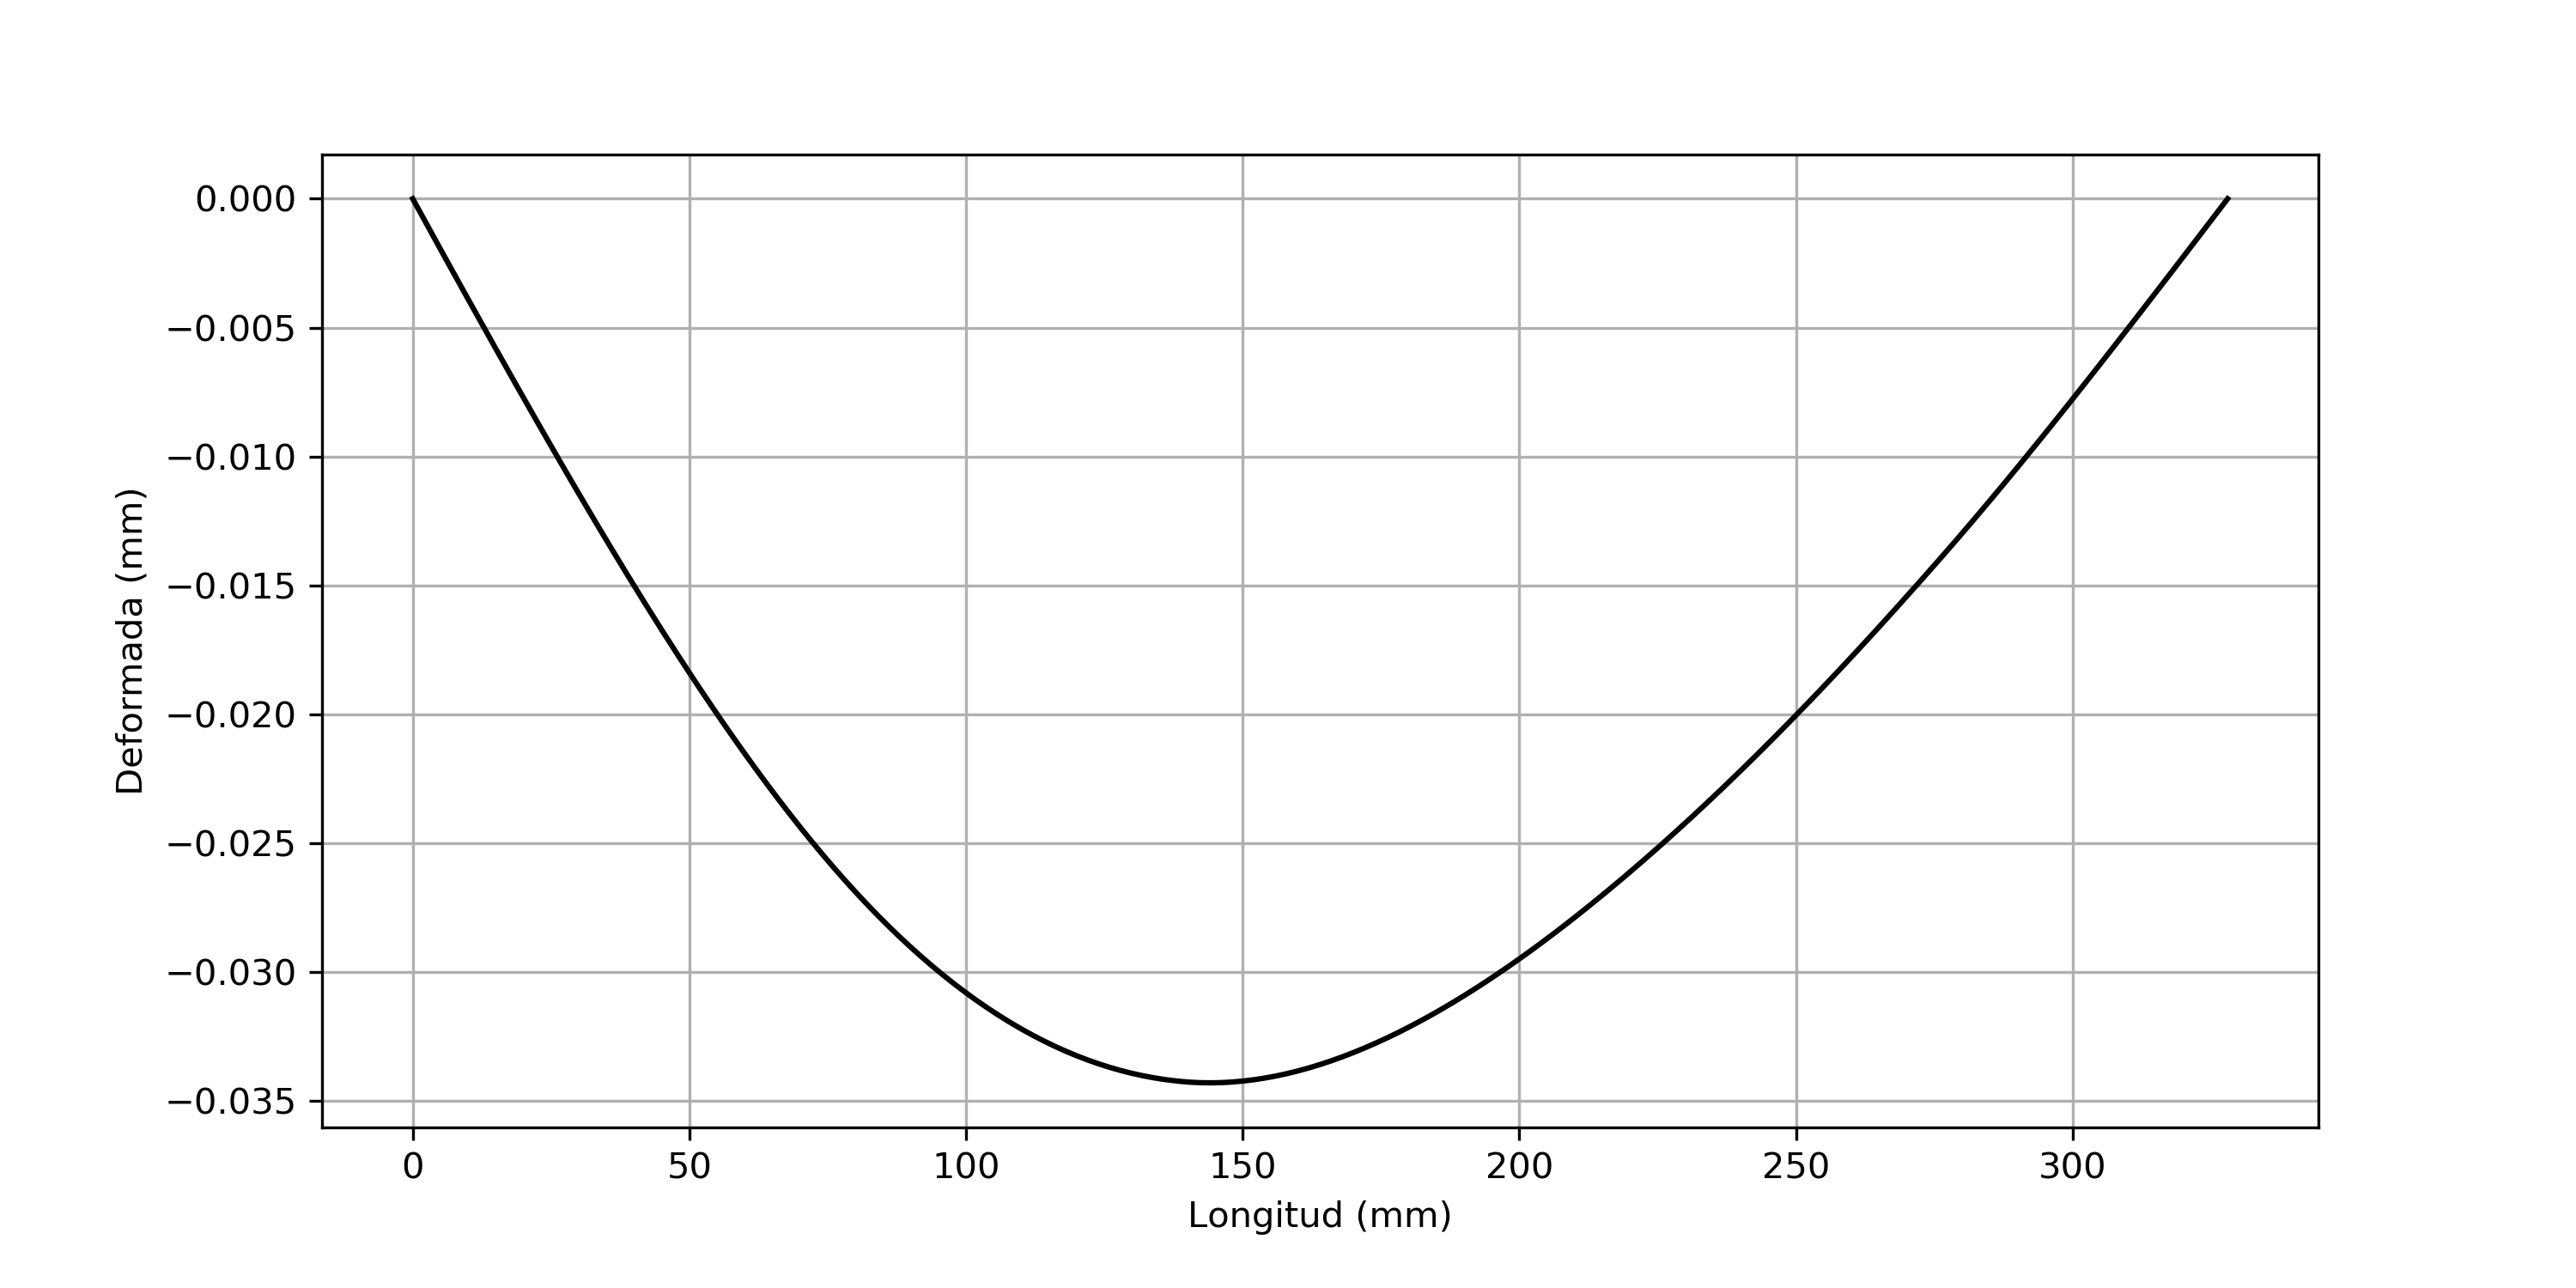
\includegraphics[scale=0.68]{defj9.png}
\caption{$n = 9$}
\end{figure}
Así mismo, podemos tomar valores muy grandes para $n$:
\begin{figure}[H]
\centering
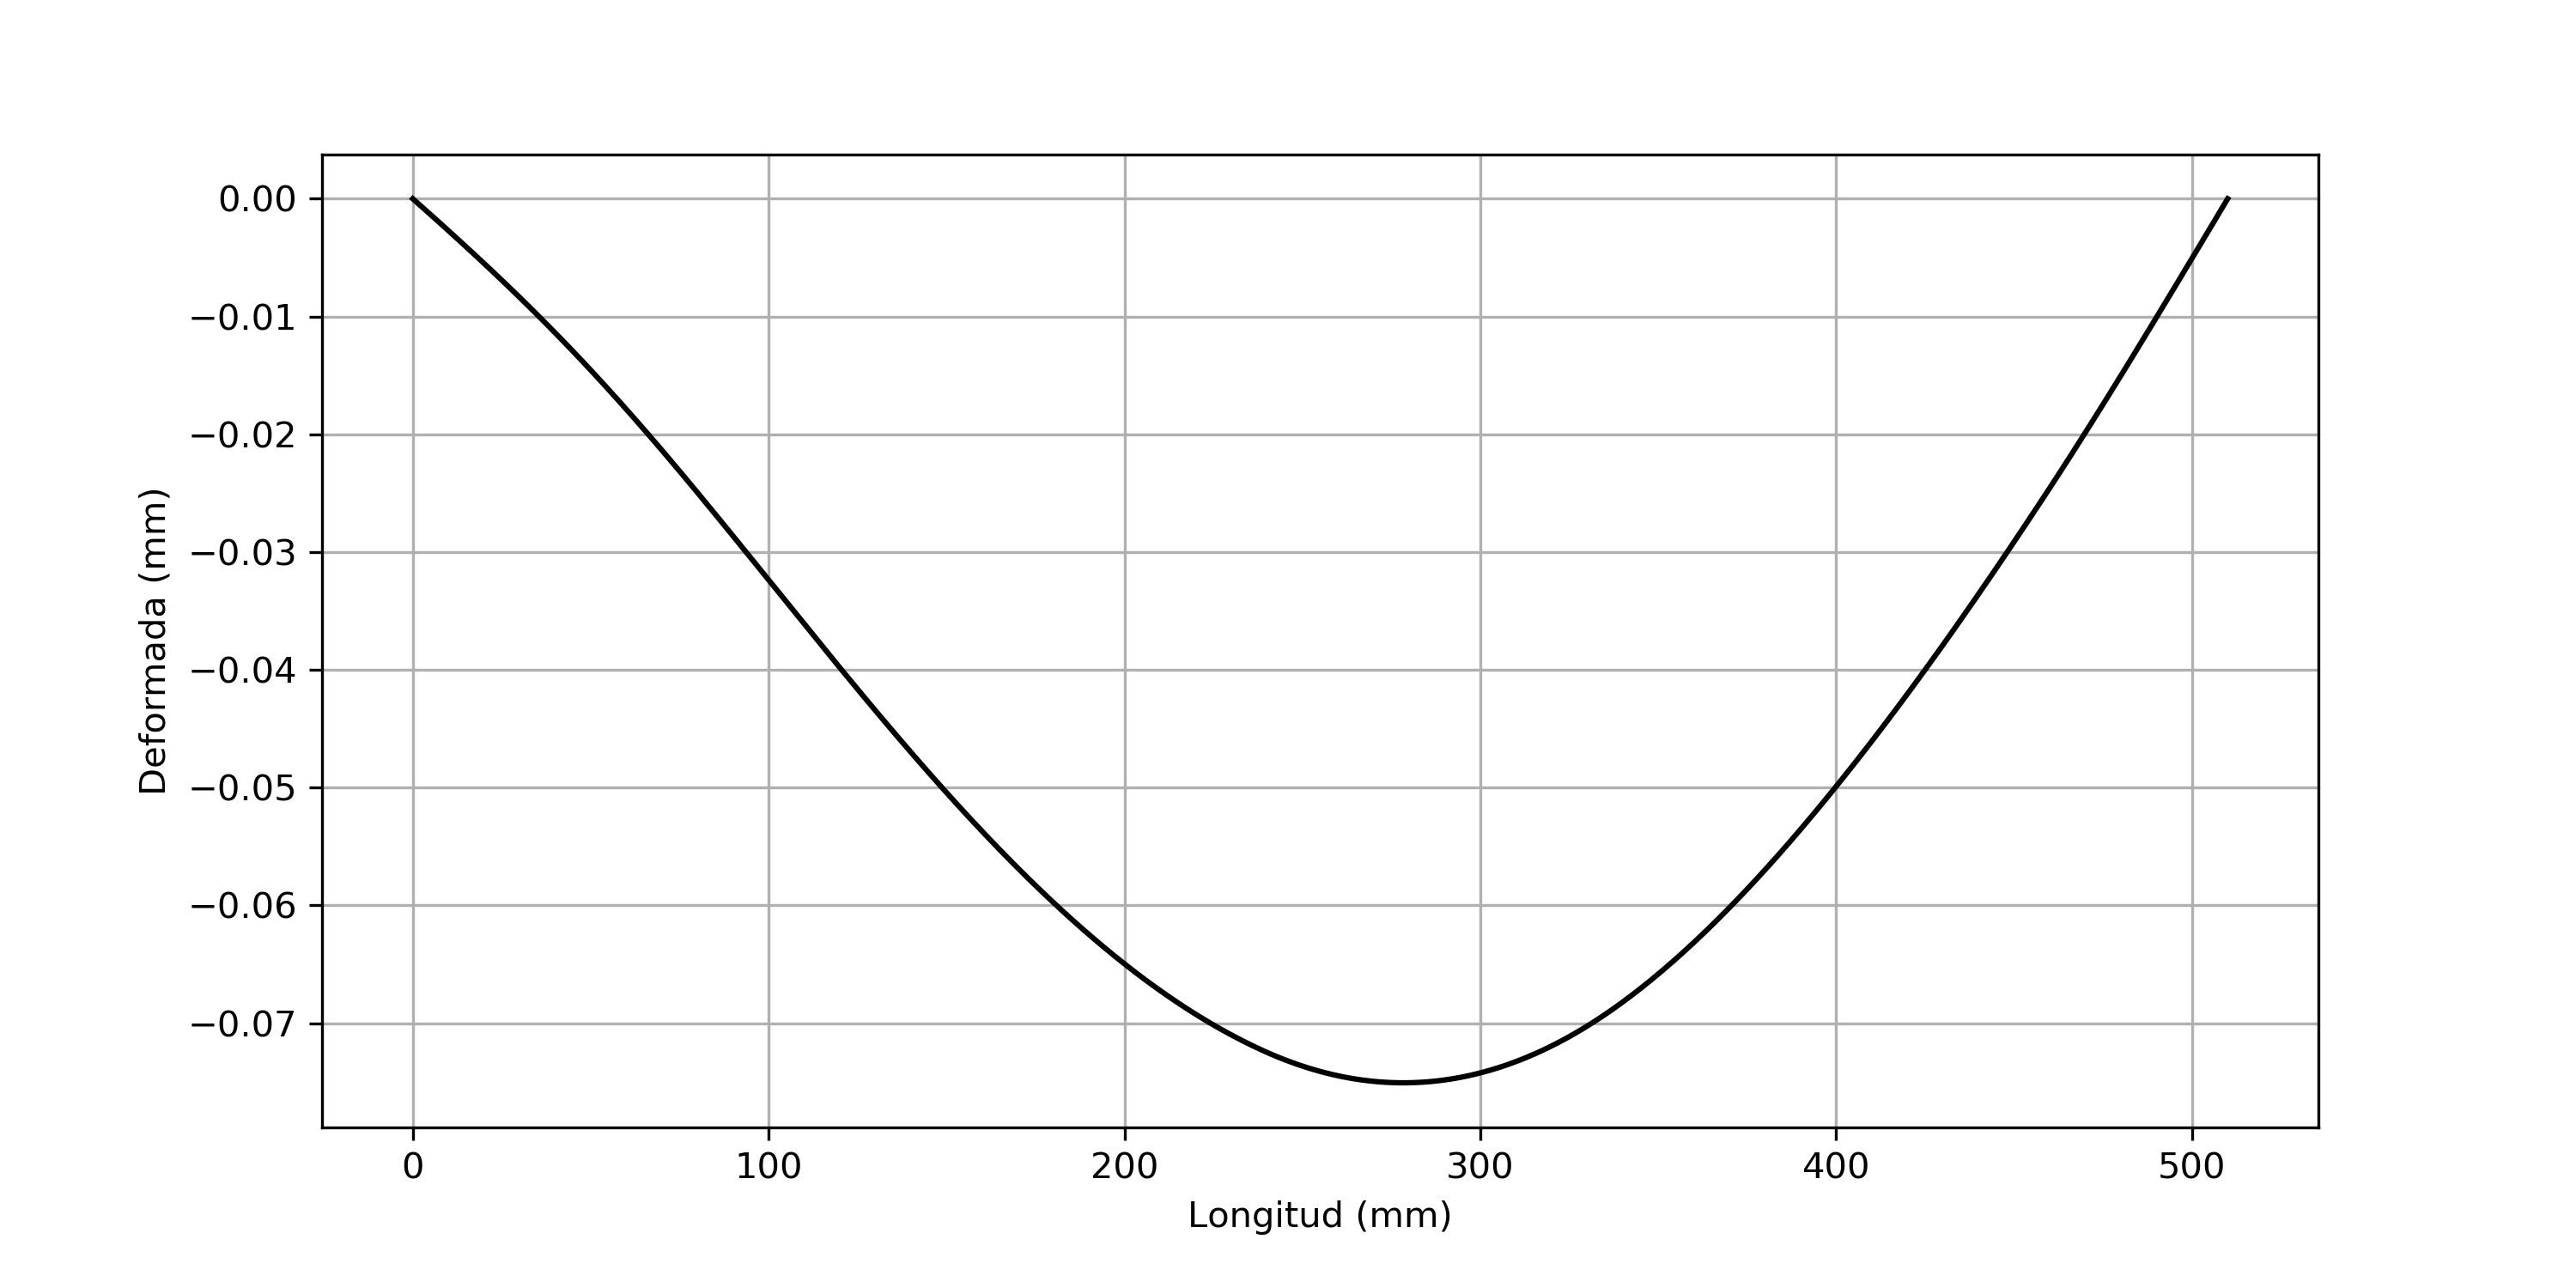
\includegraphics[scale=0.68]{defj100.png}
\caption{$n = 100$}
\end{figure}
\begin{figure}[H]
\centering
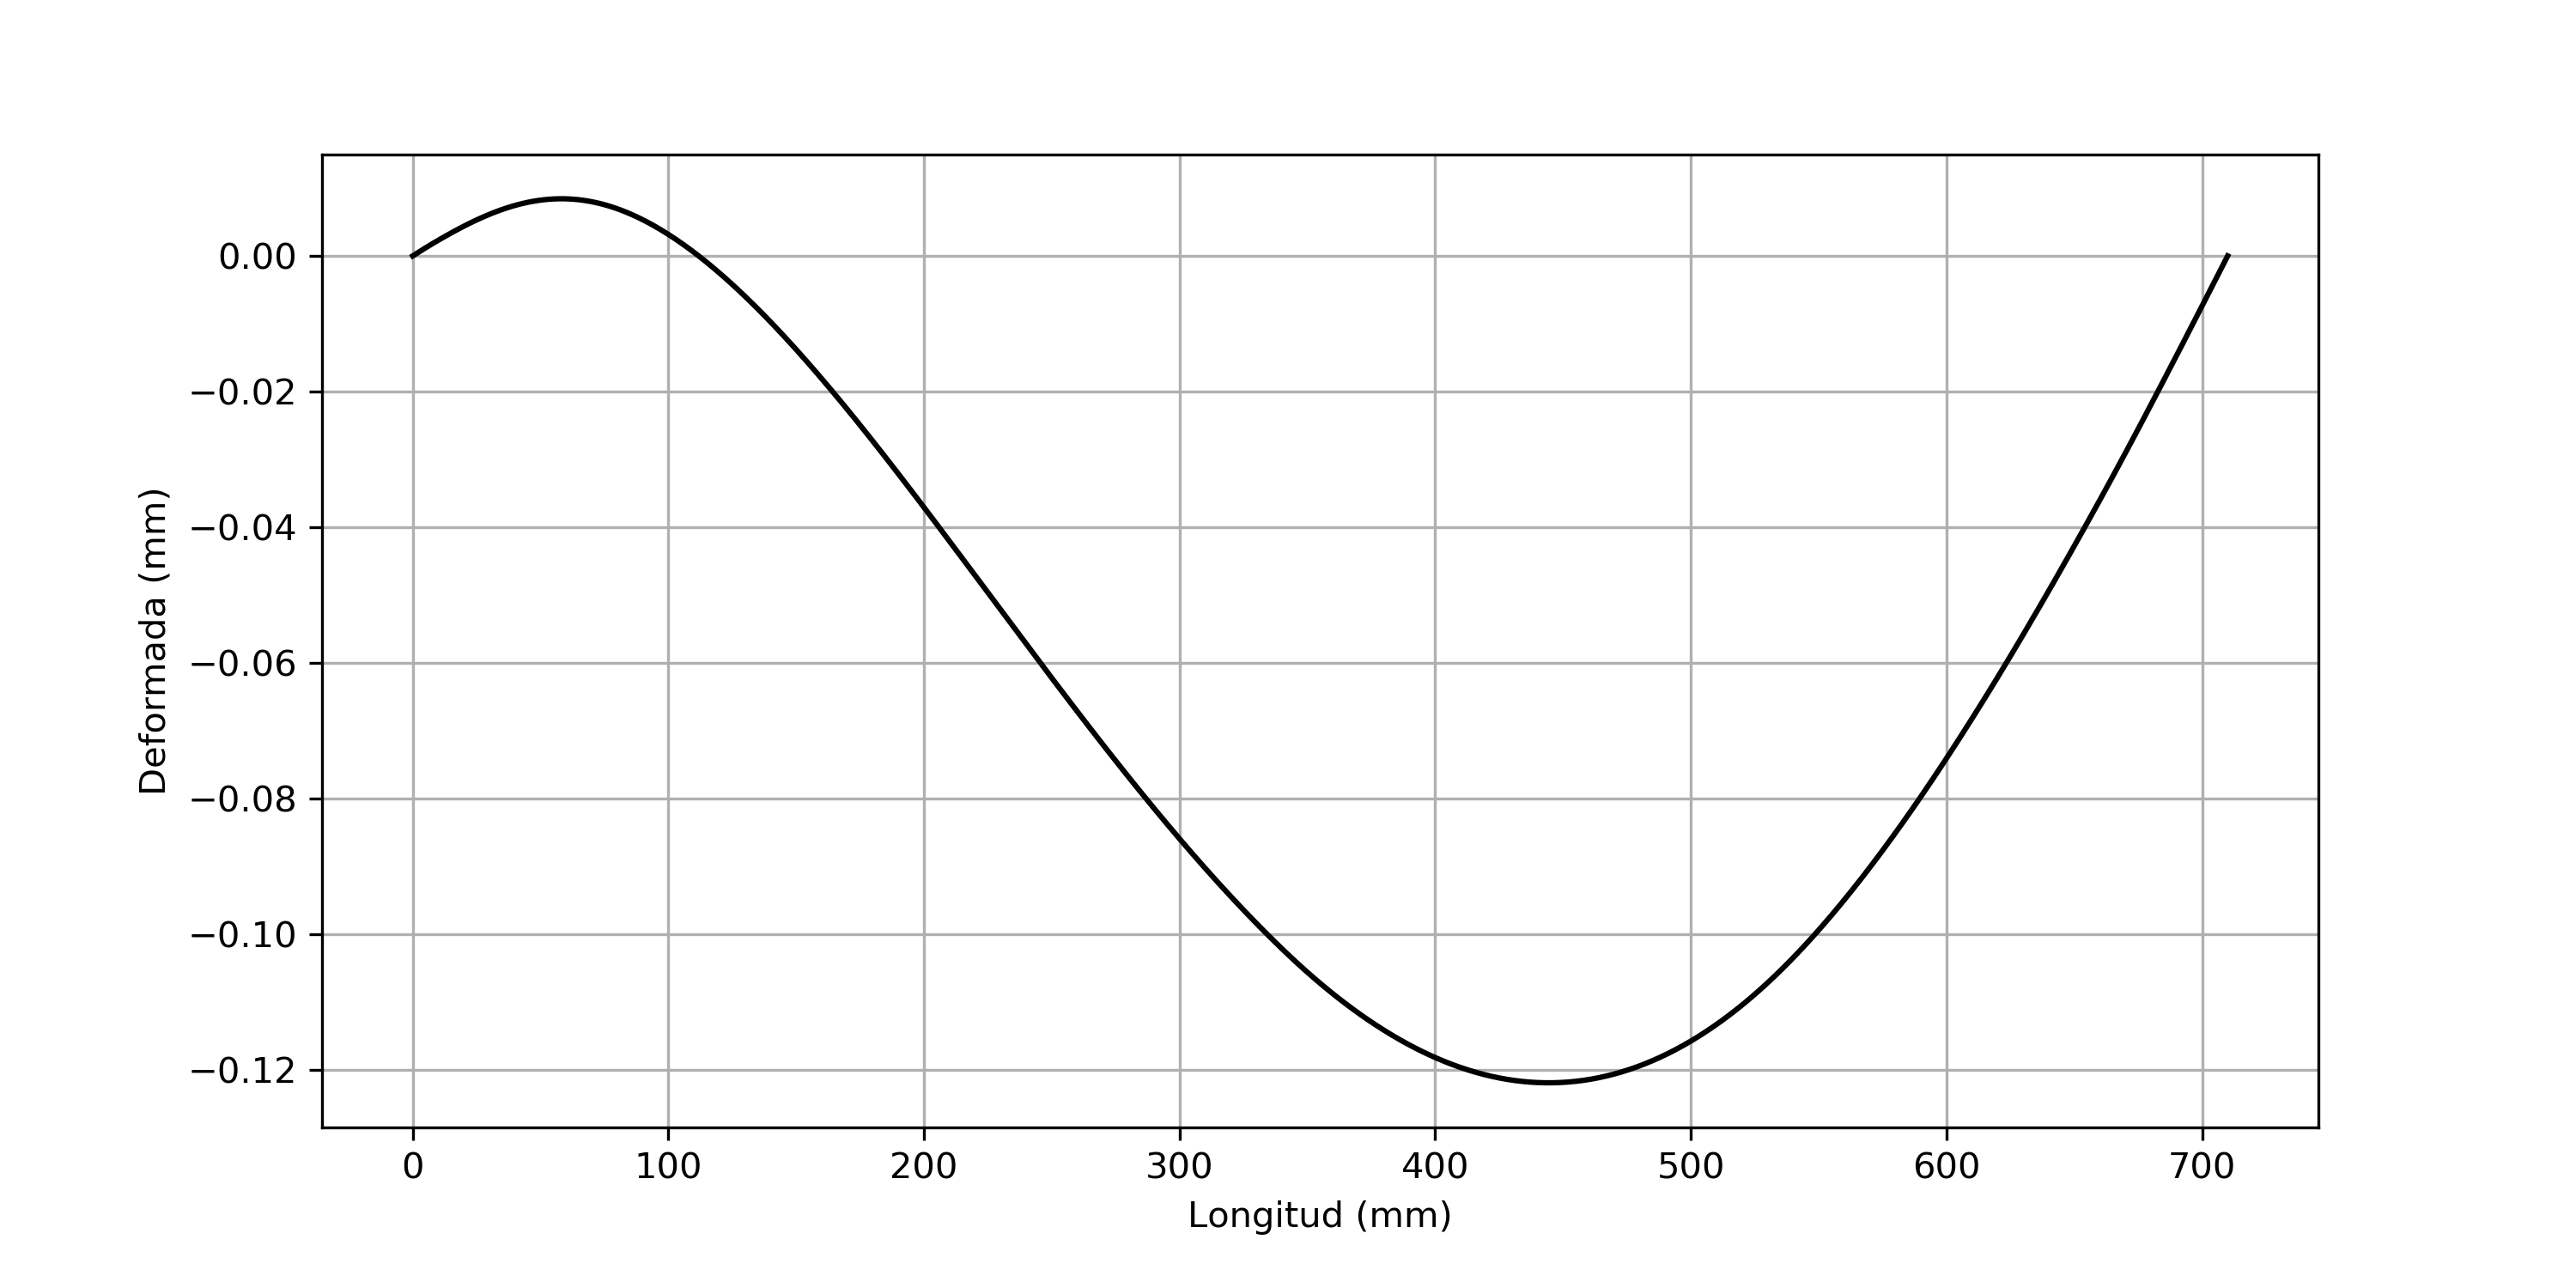
\includegraphics[scale=0.68]{defj200.png}
\caption{$n = 200$}
\end{figure}
\begin{figure}[H]
\centering
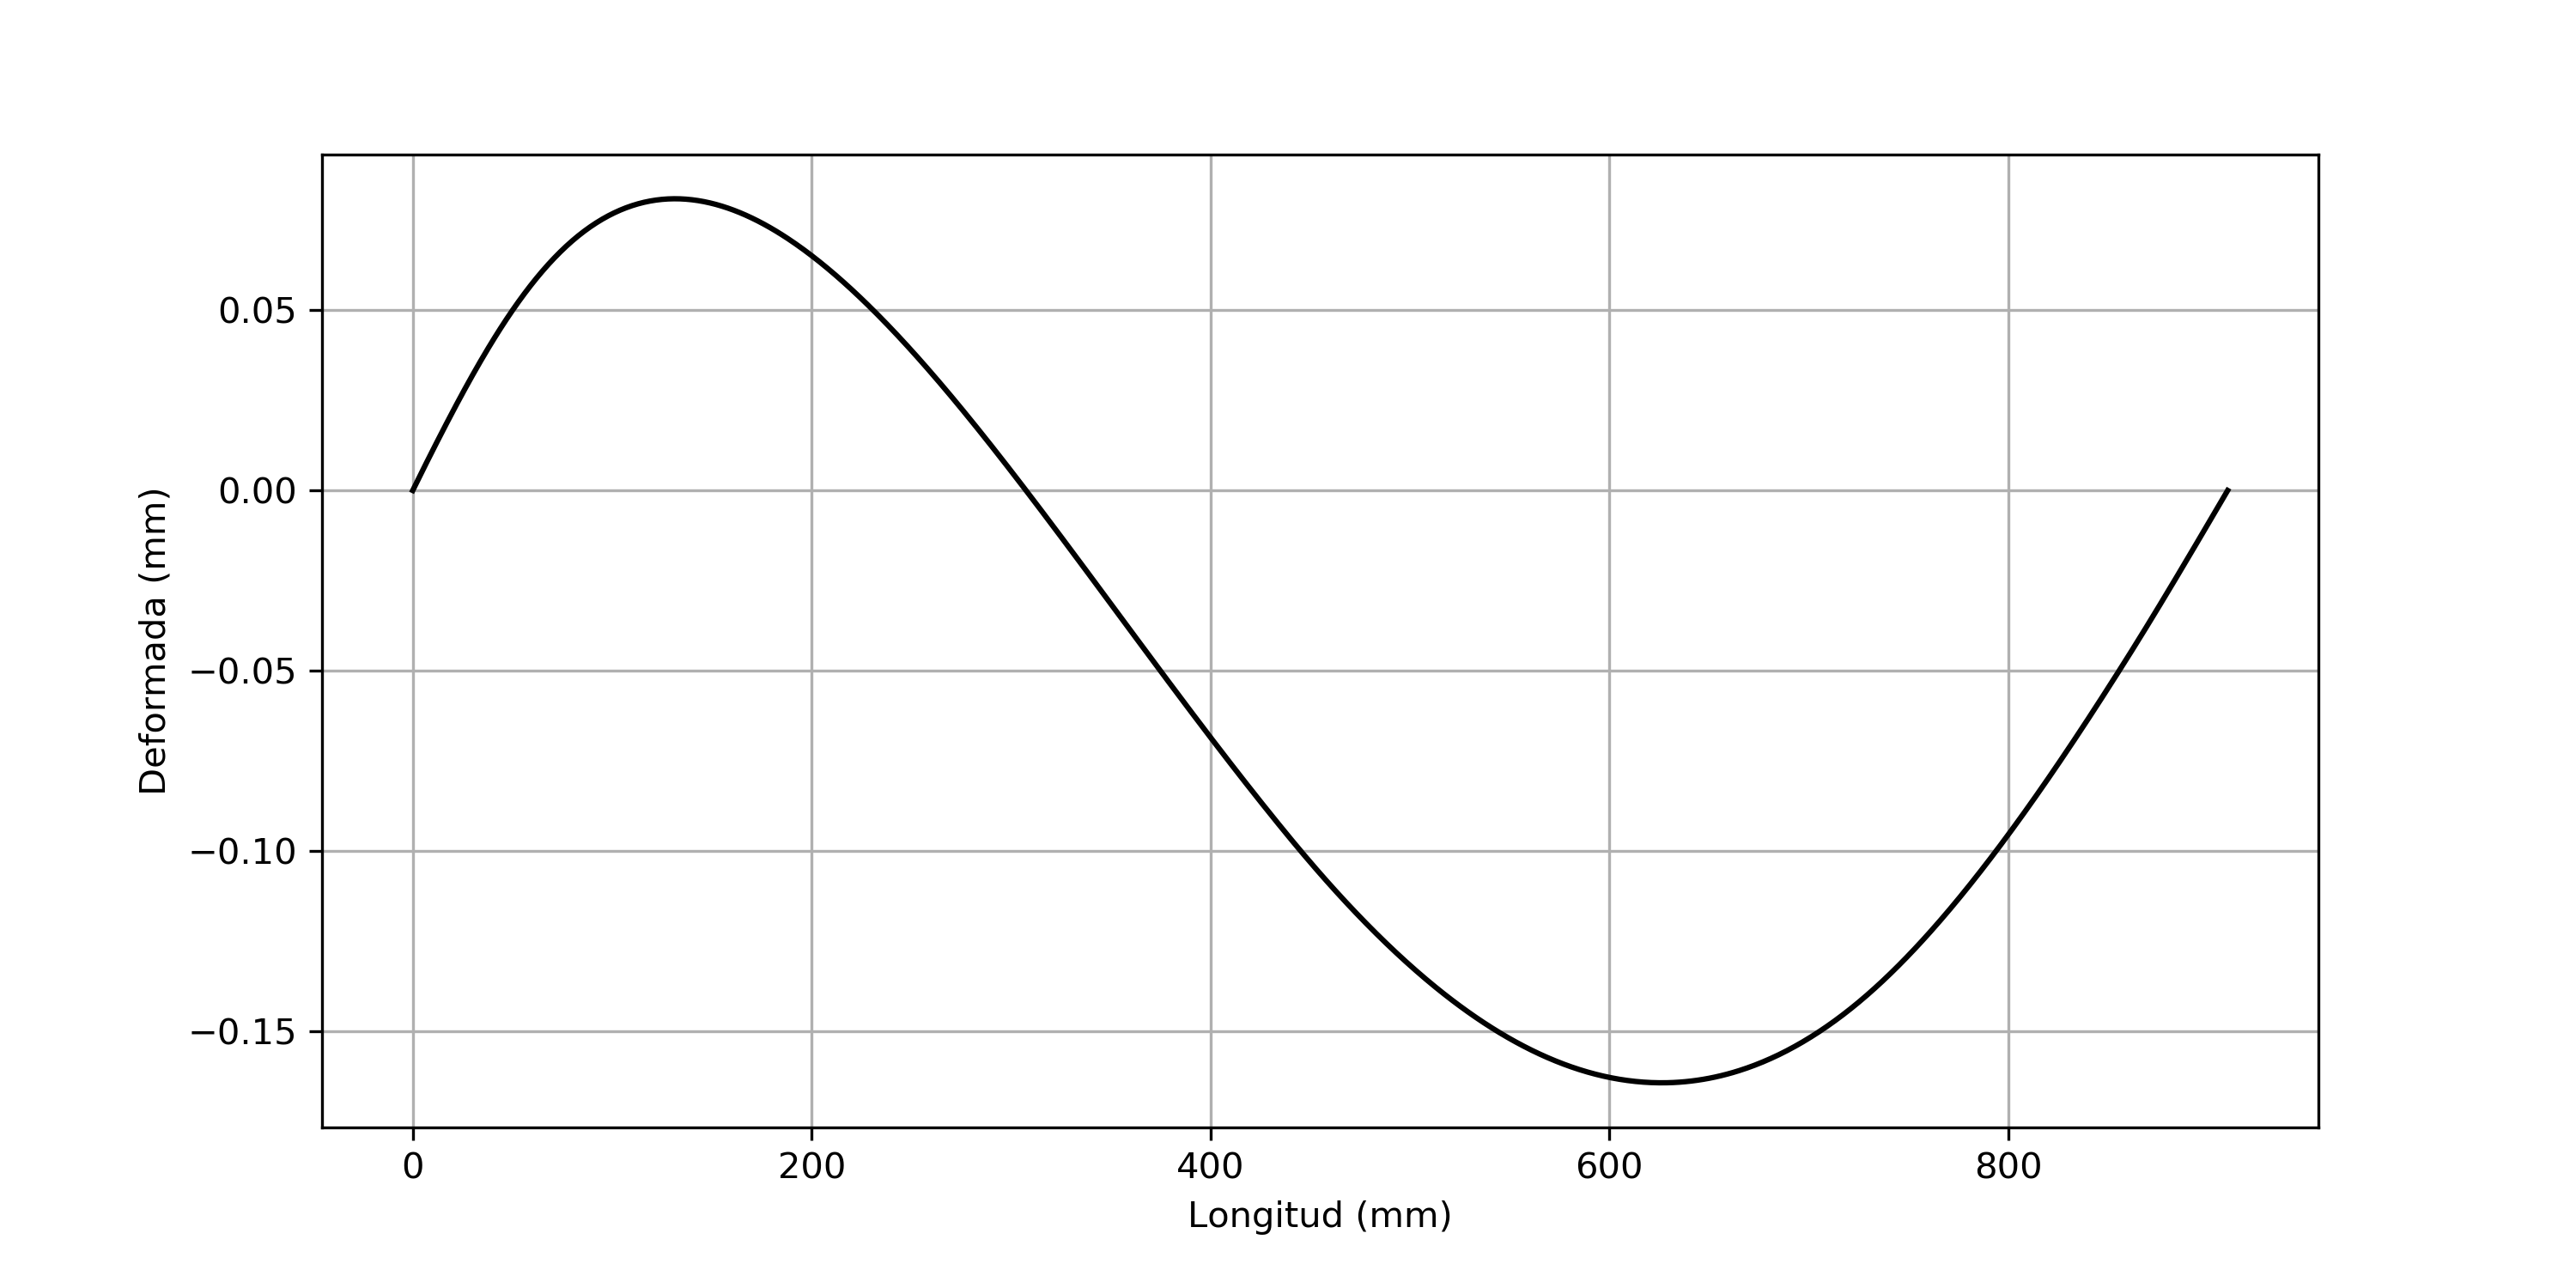
\includegraphics[scale=0.68]{defj300.png}
\caption{$n = 300$}
\end{figure}
\begin{figure}[H]
\centering
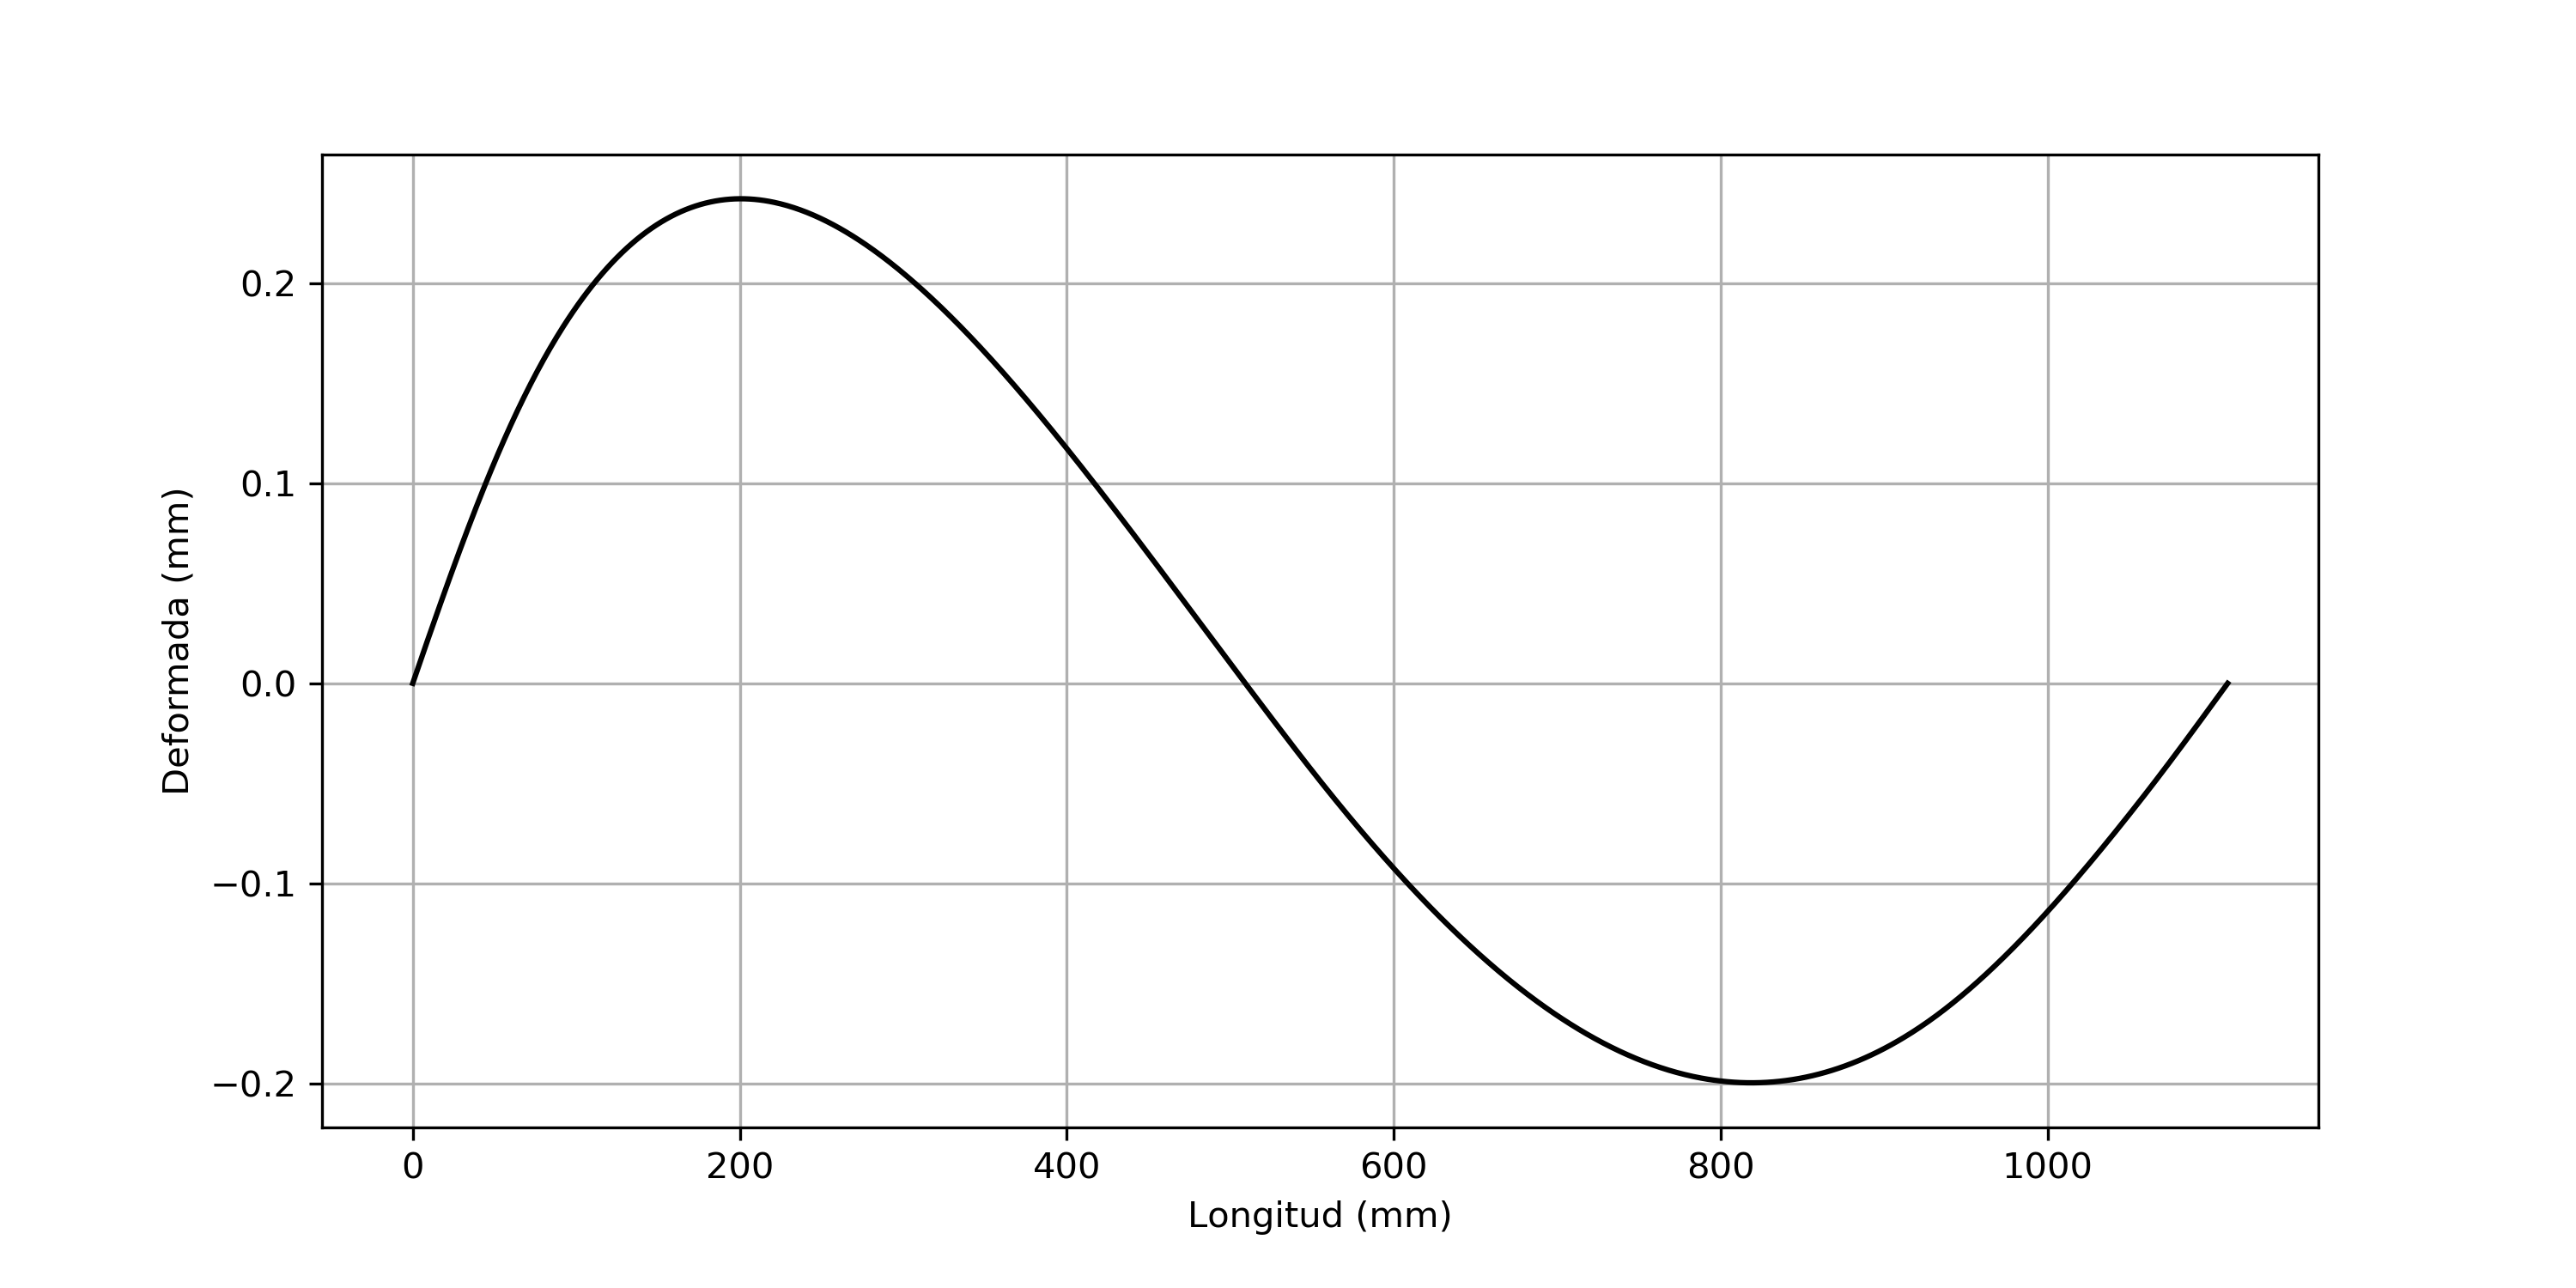
\includegraphics[scale=0.68]{defj400.png}
\caption{$n = 400$}
\end{figure}
\begin{figure}[H]
\centering
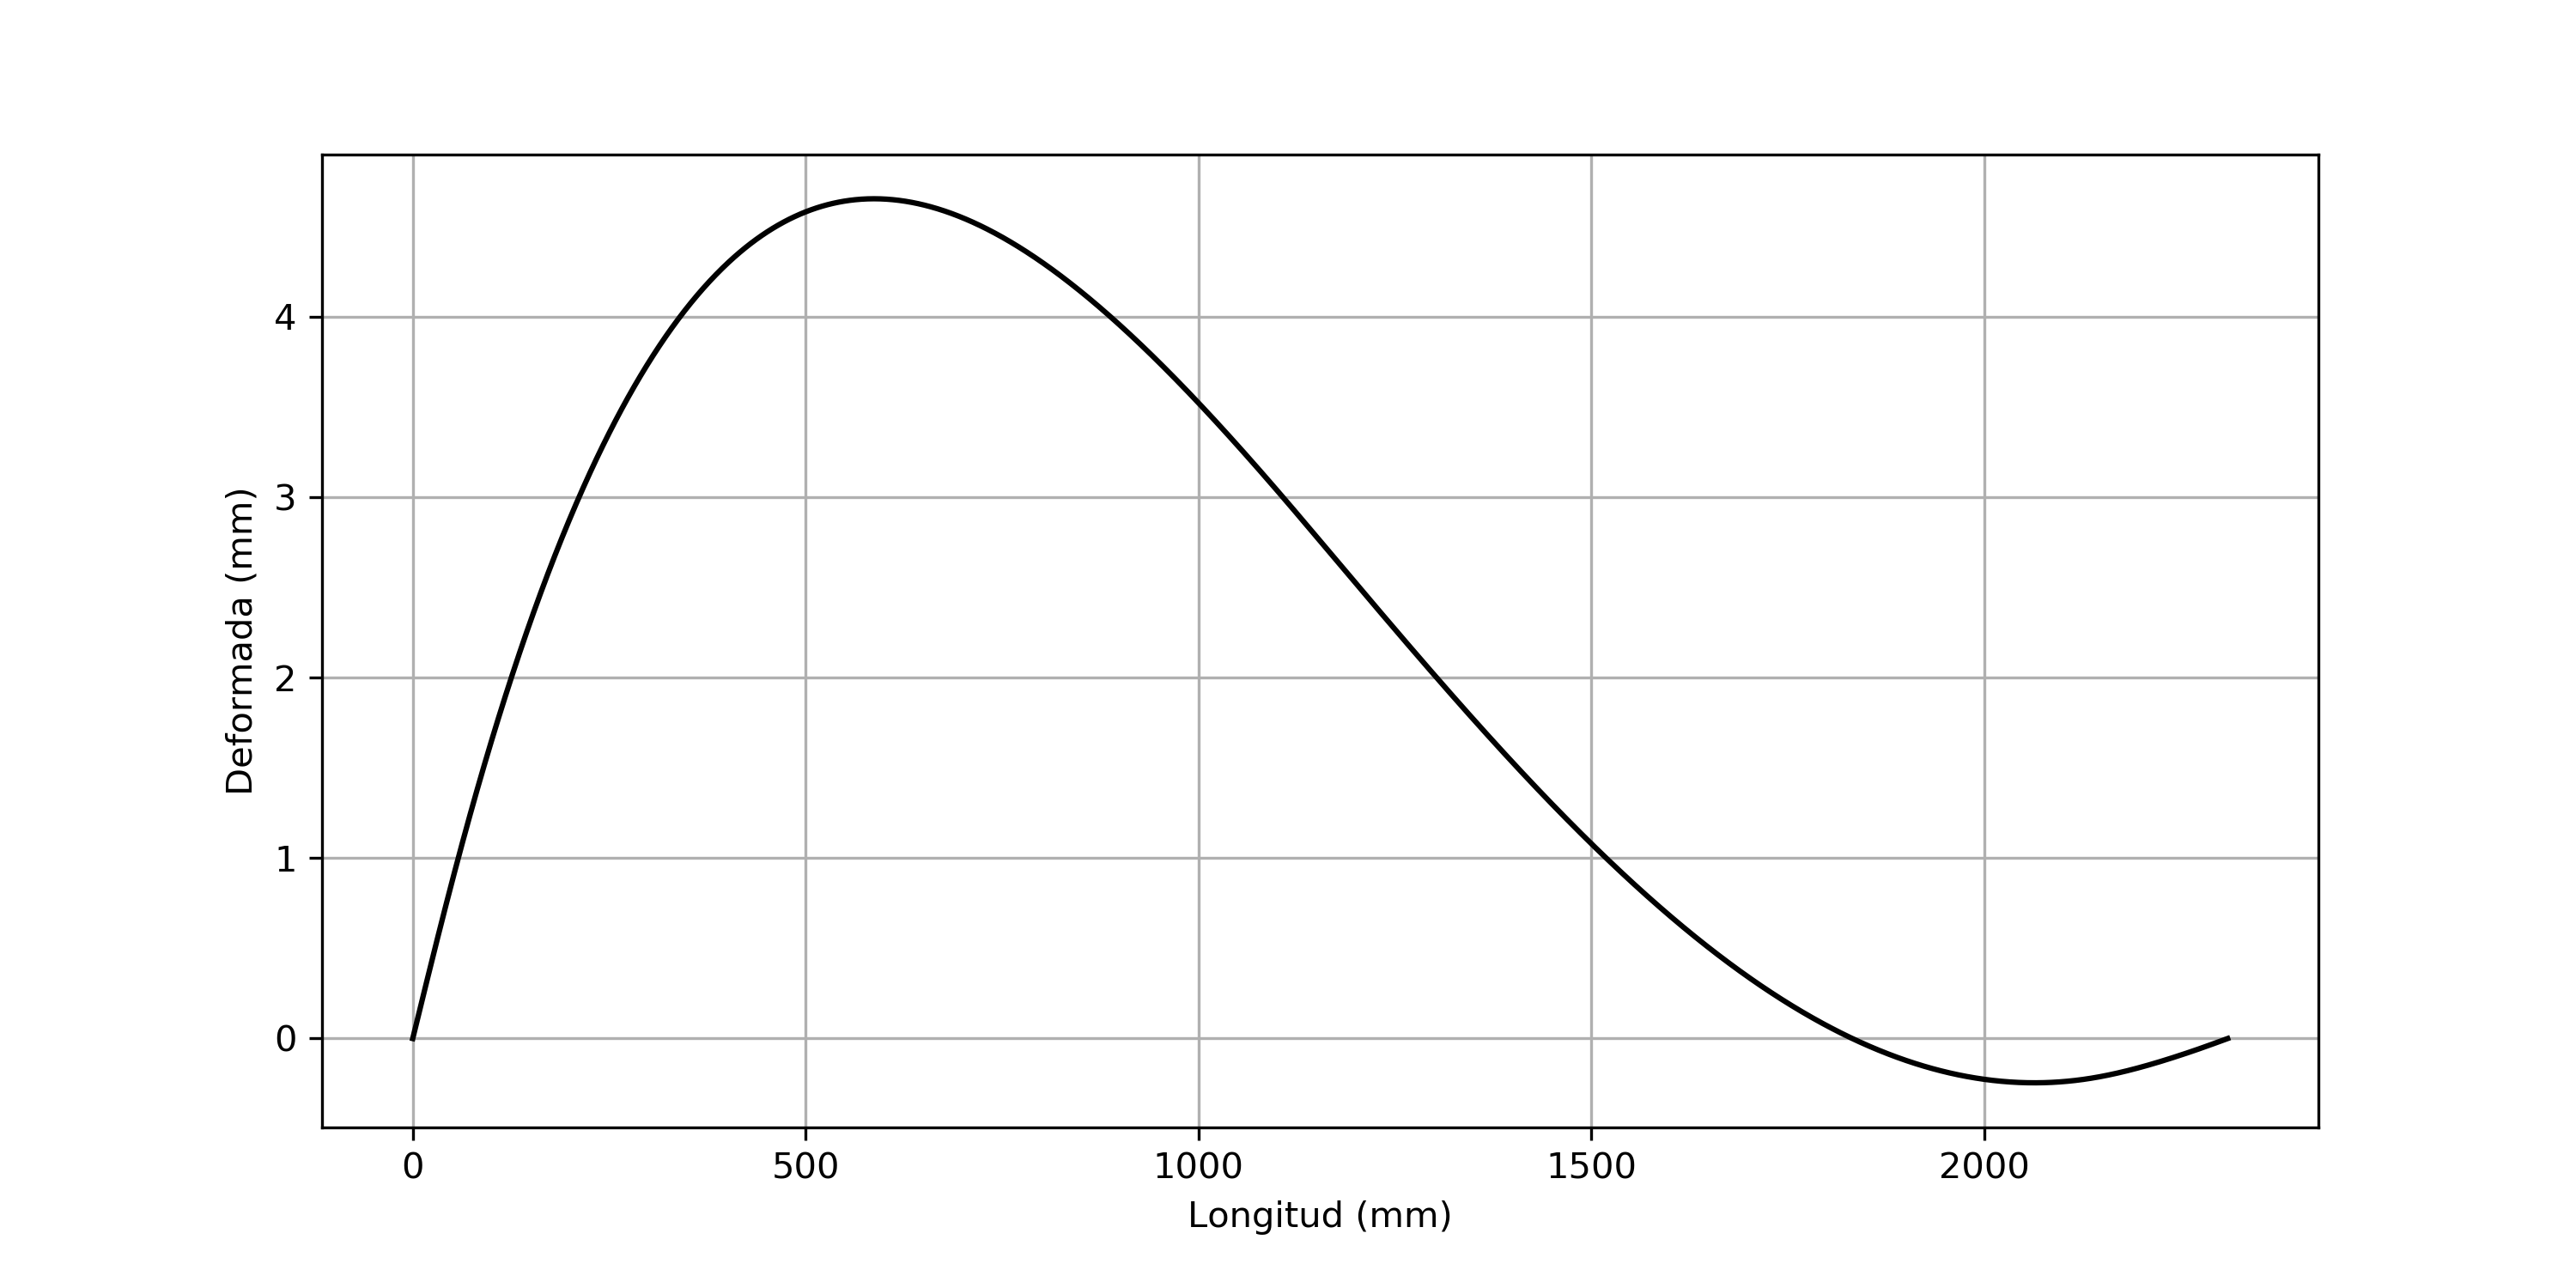
\includegraphics[scale=0.68]{defj1000.png}
\caption{$n = 1000$}
\end{figure}
\begin{figure}[H]
\centering
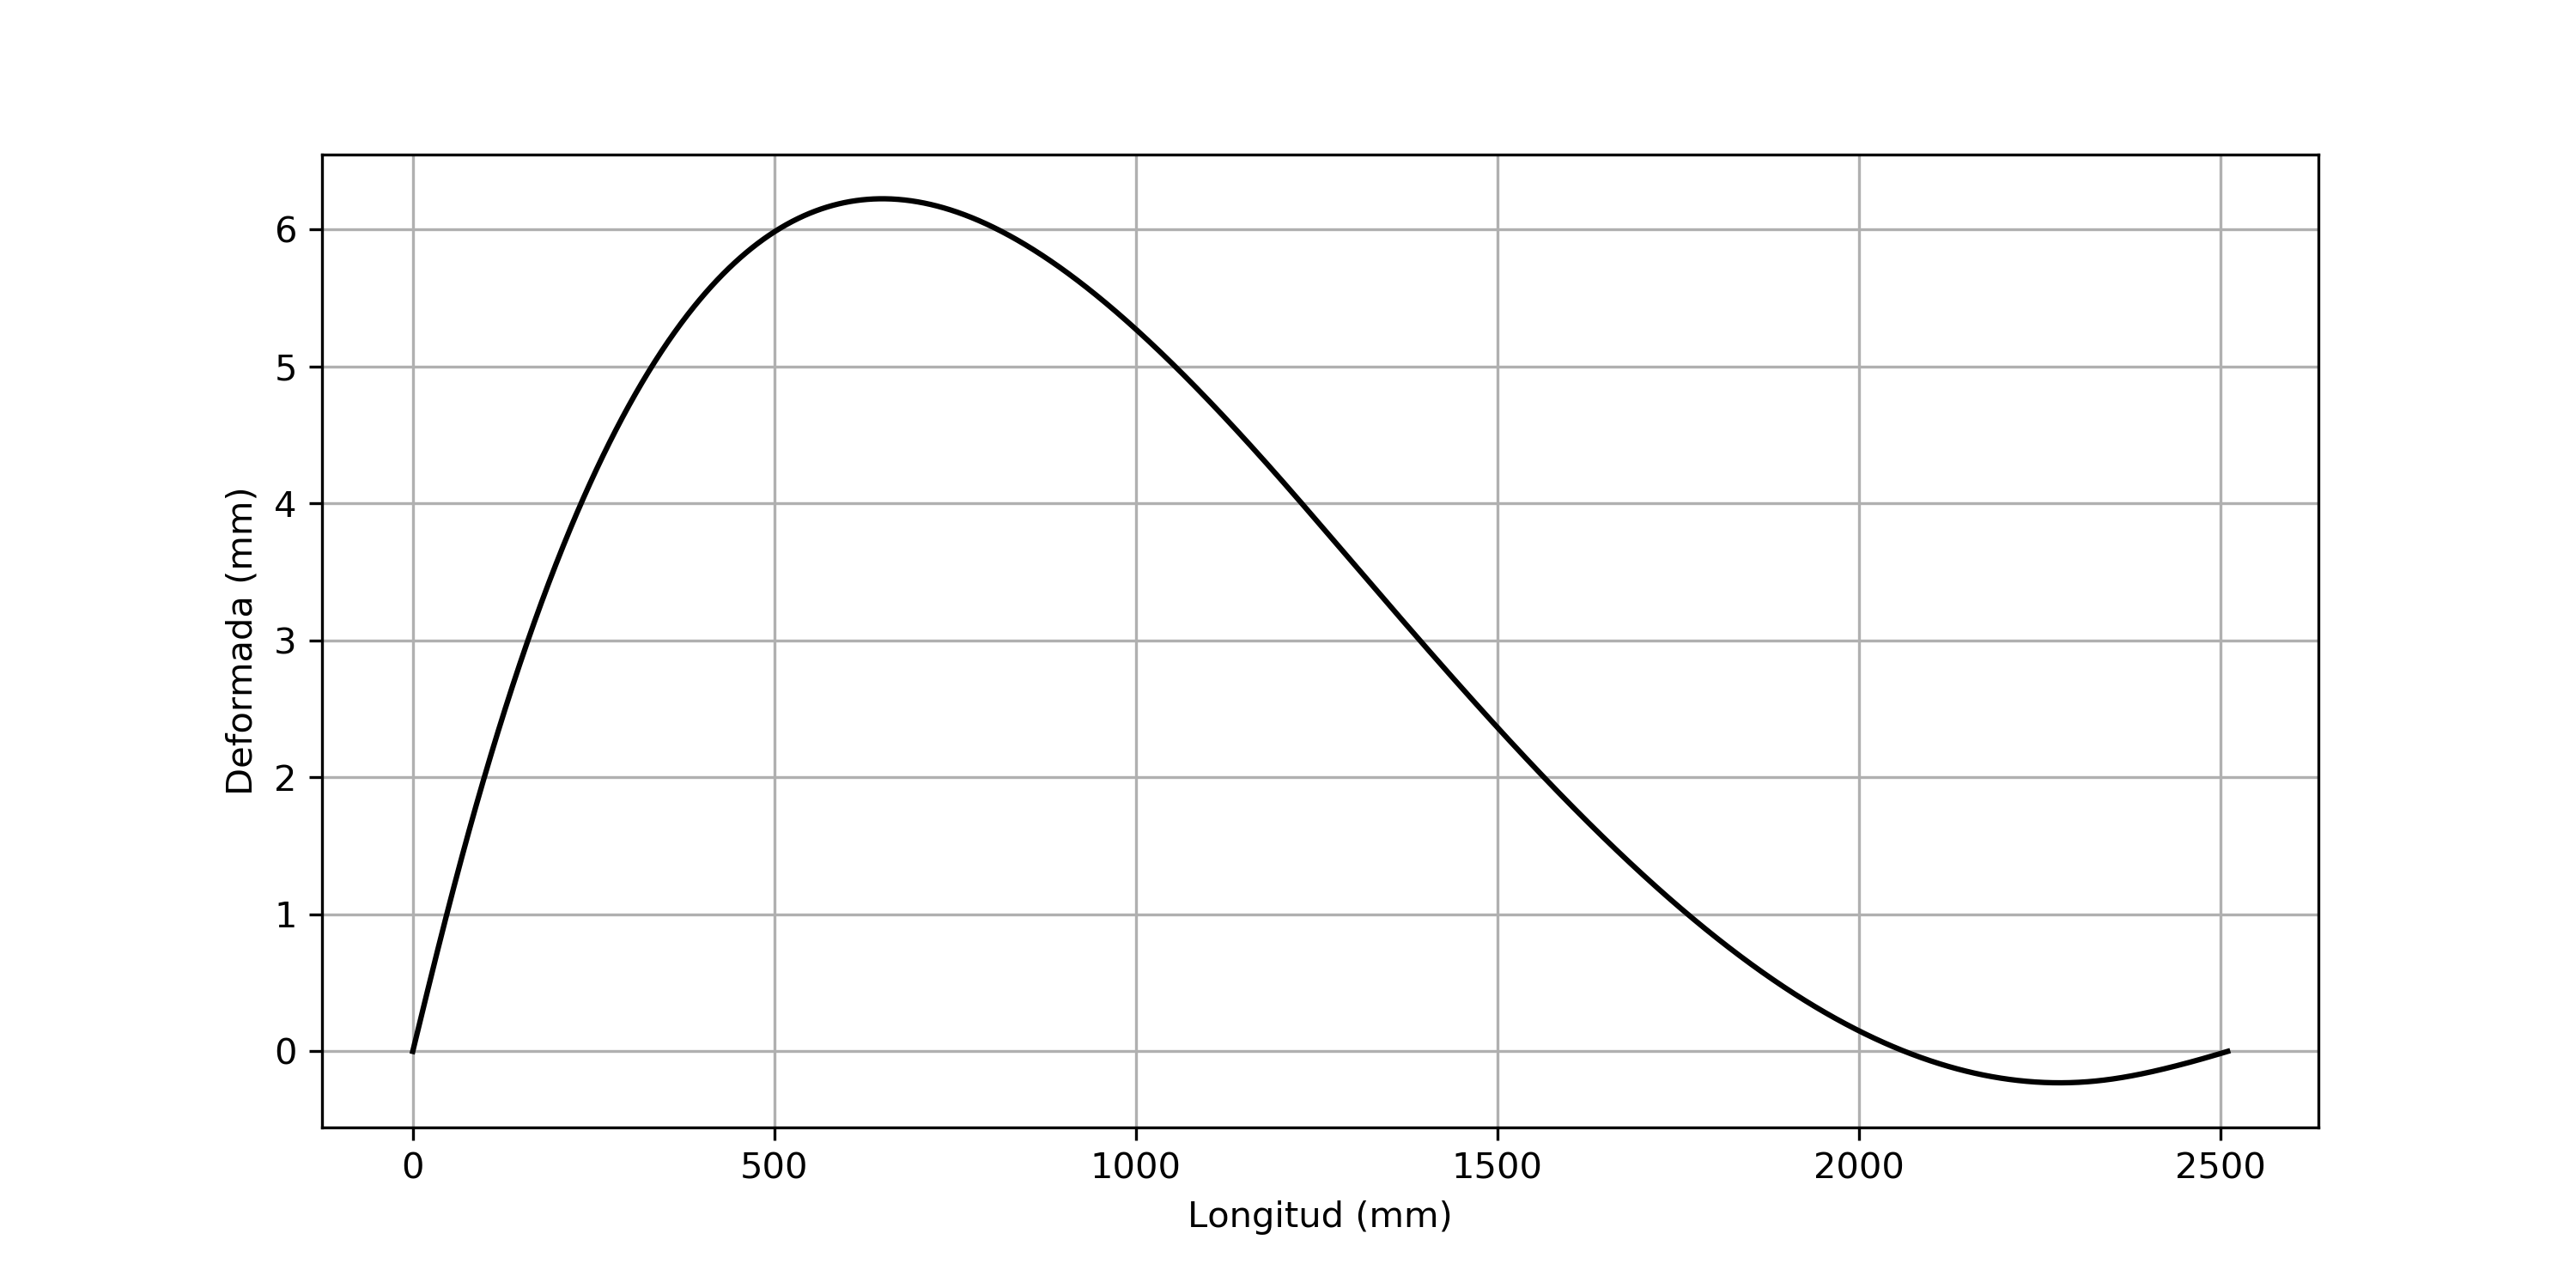
\includegraphics[scale=0.68]{defj1100.png}
\caption{$n = 1100$}
\end{figure}
\begin{figure}[H]
\centering
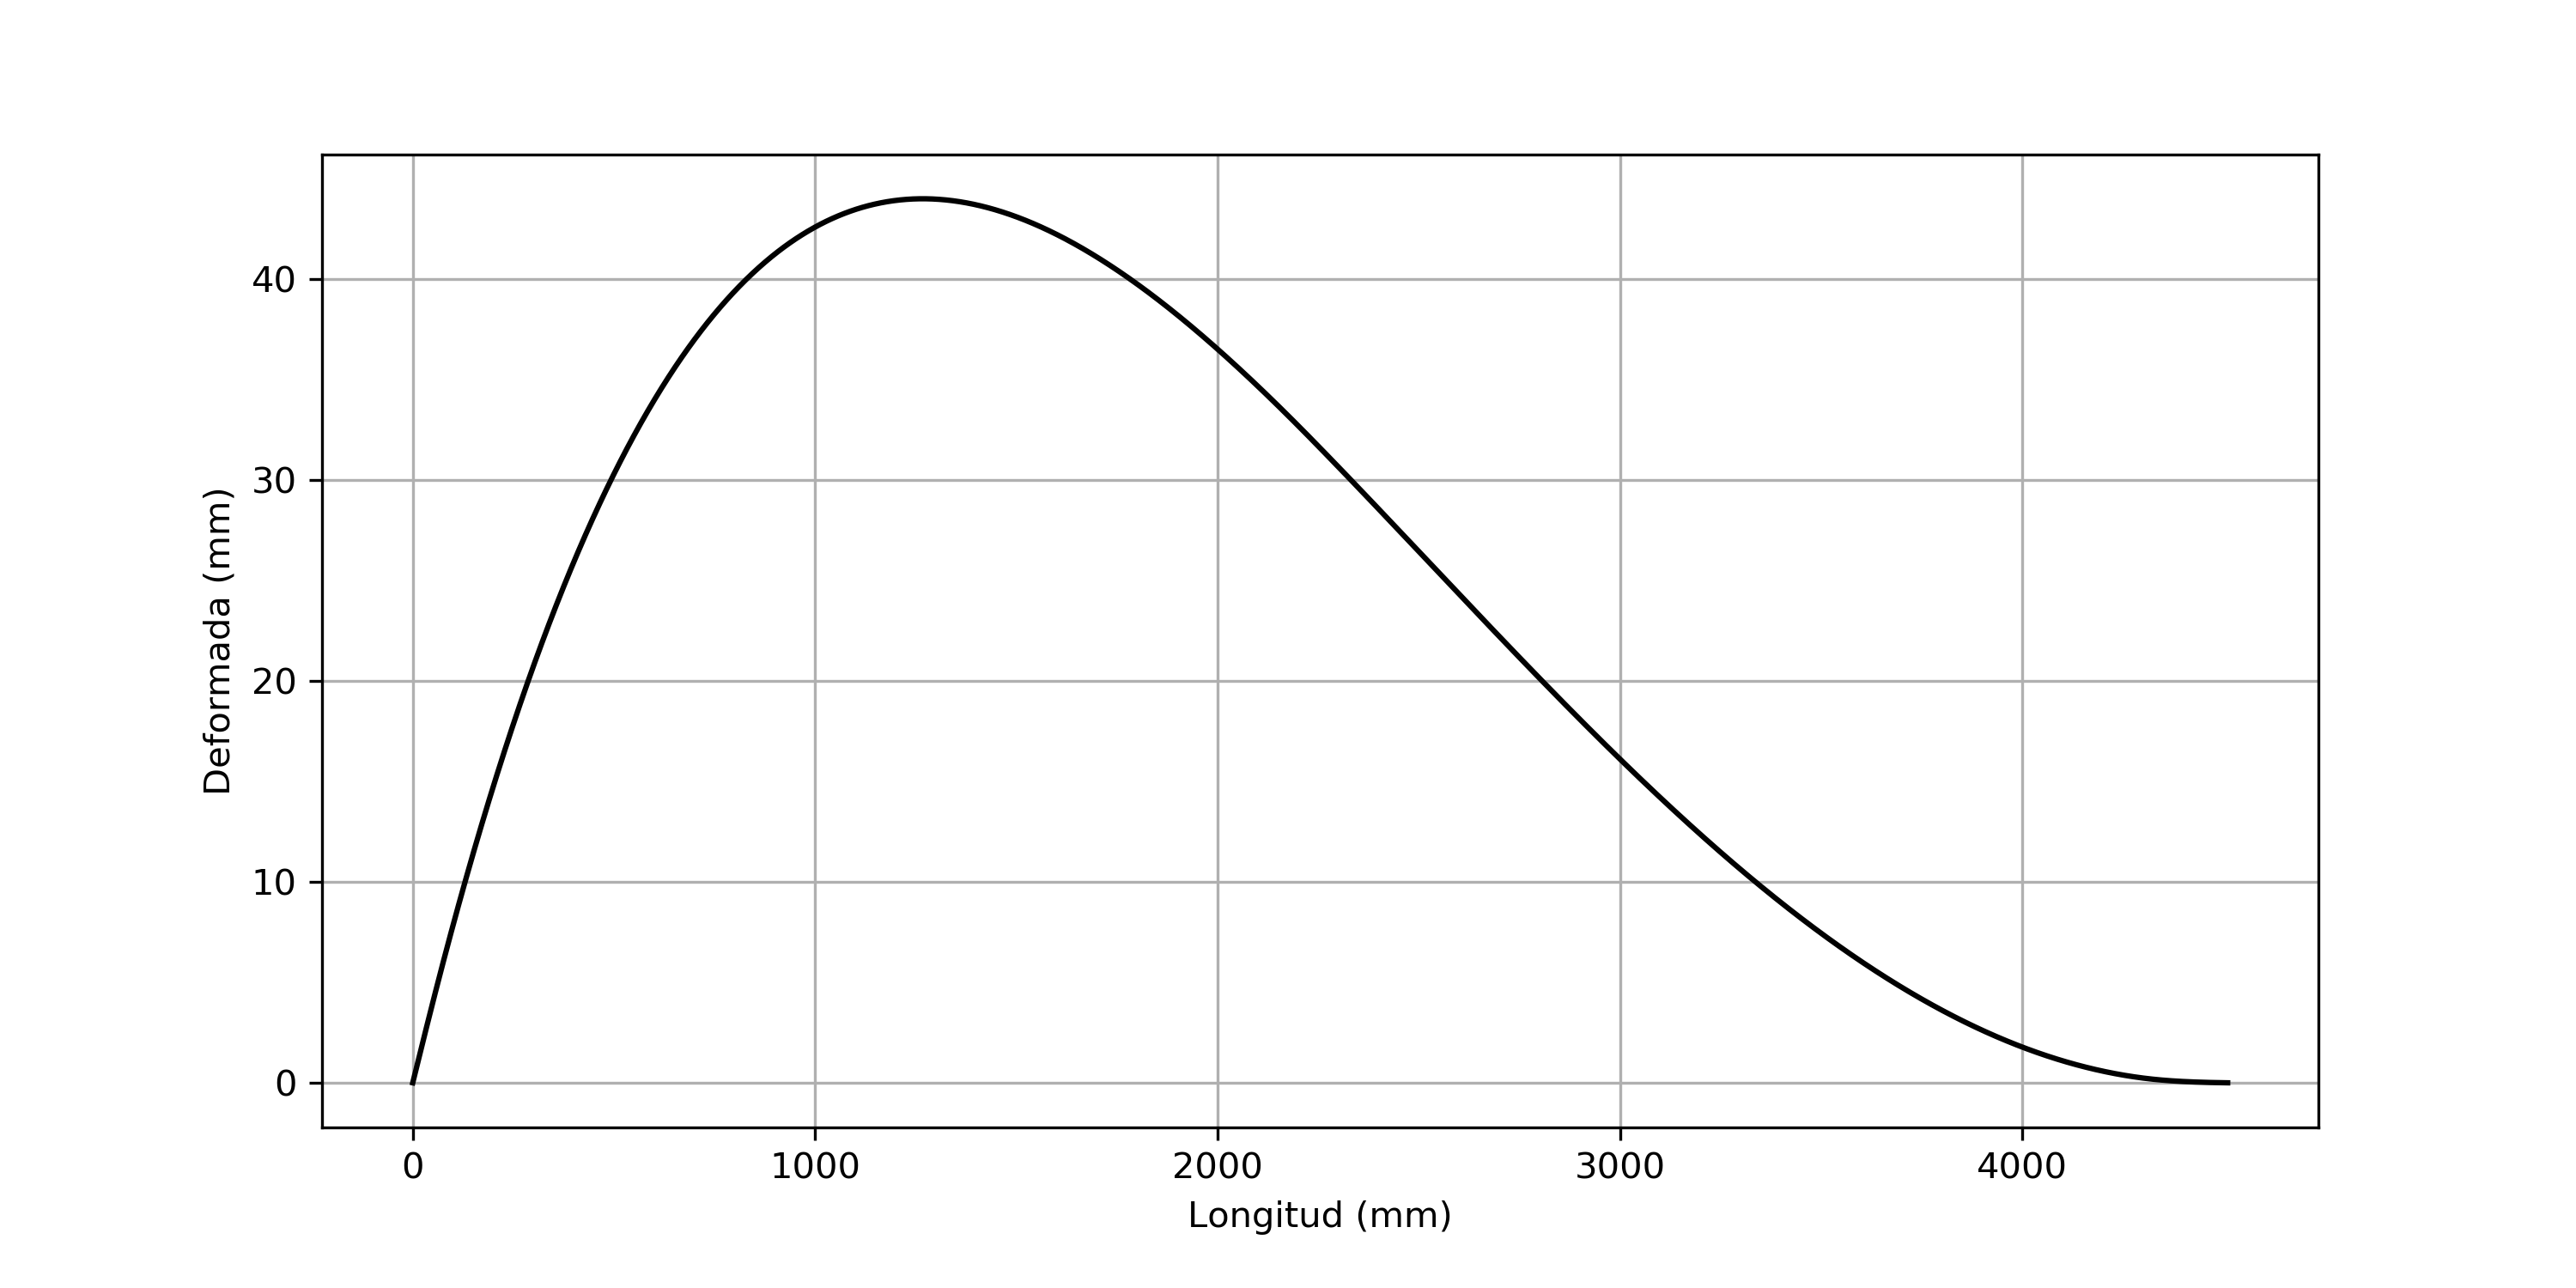
\includegraphics[scale=0.68]{defj2100.png}
\caption{$n = 2100$}
\end{figure}
\begin{figure}[H]
\centering
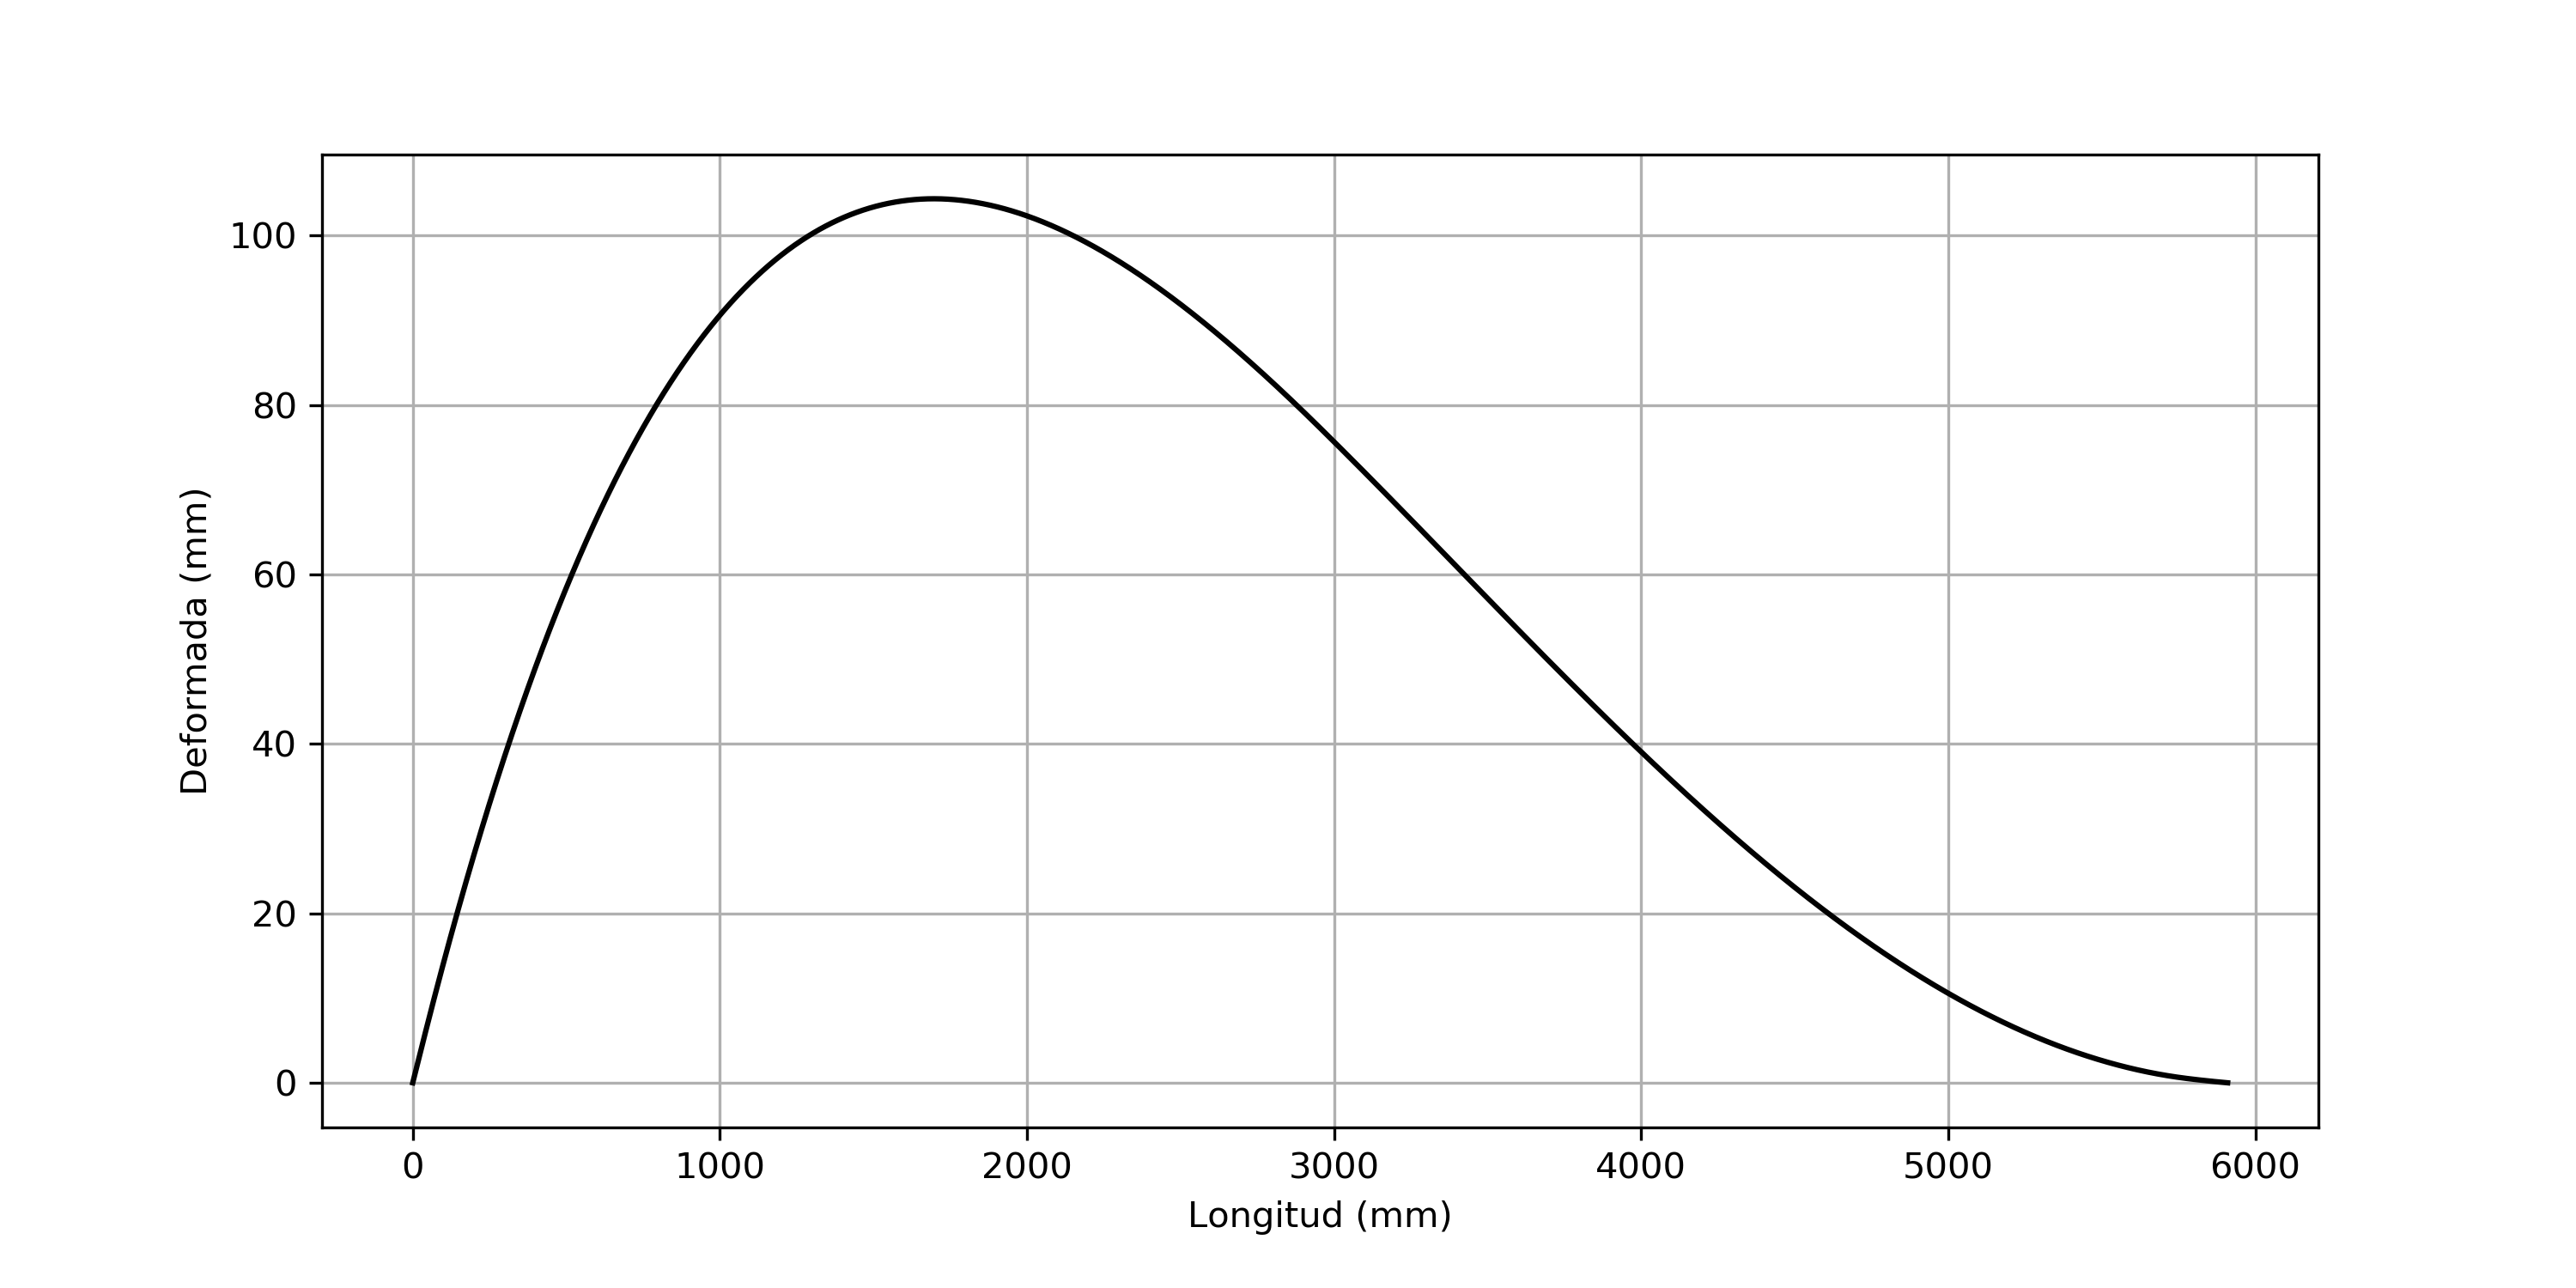
\includegraphics[scale=0.68]{defj2800.png}
\caption{$n = 2800$}
\end{figure}
\begin{figure}[H]
\centering
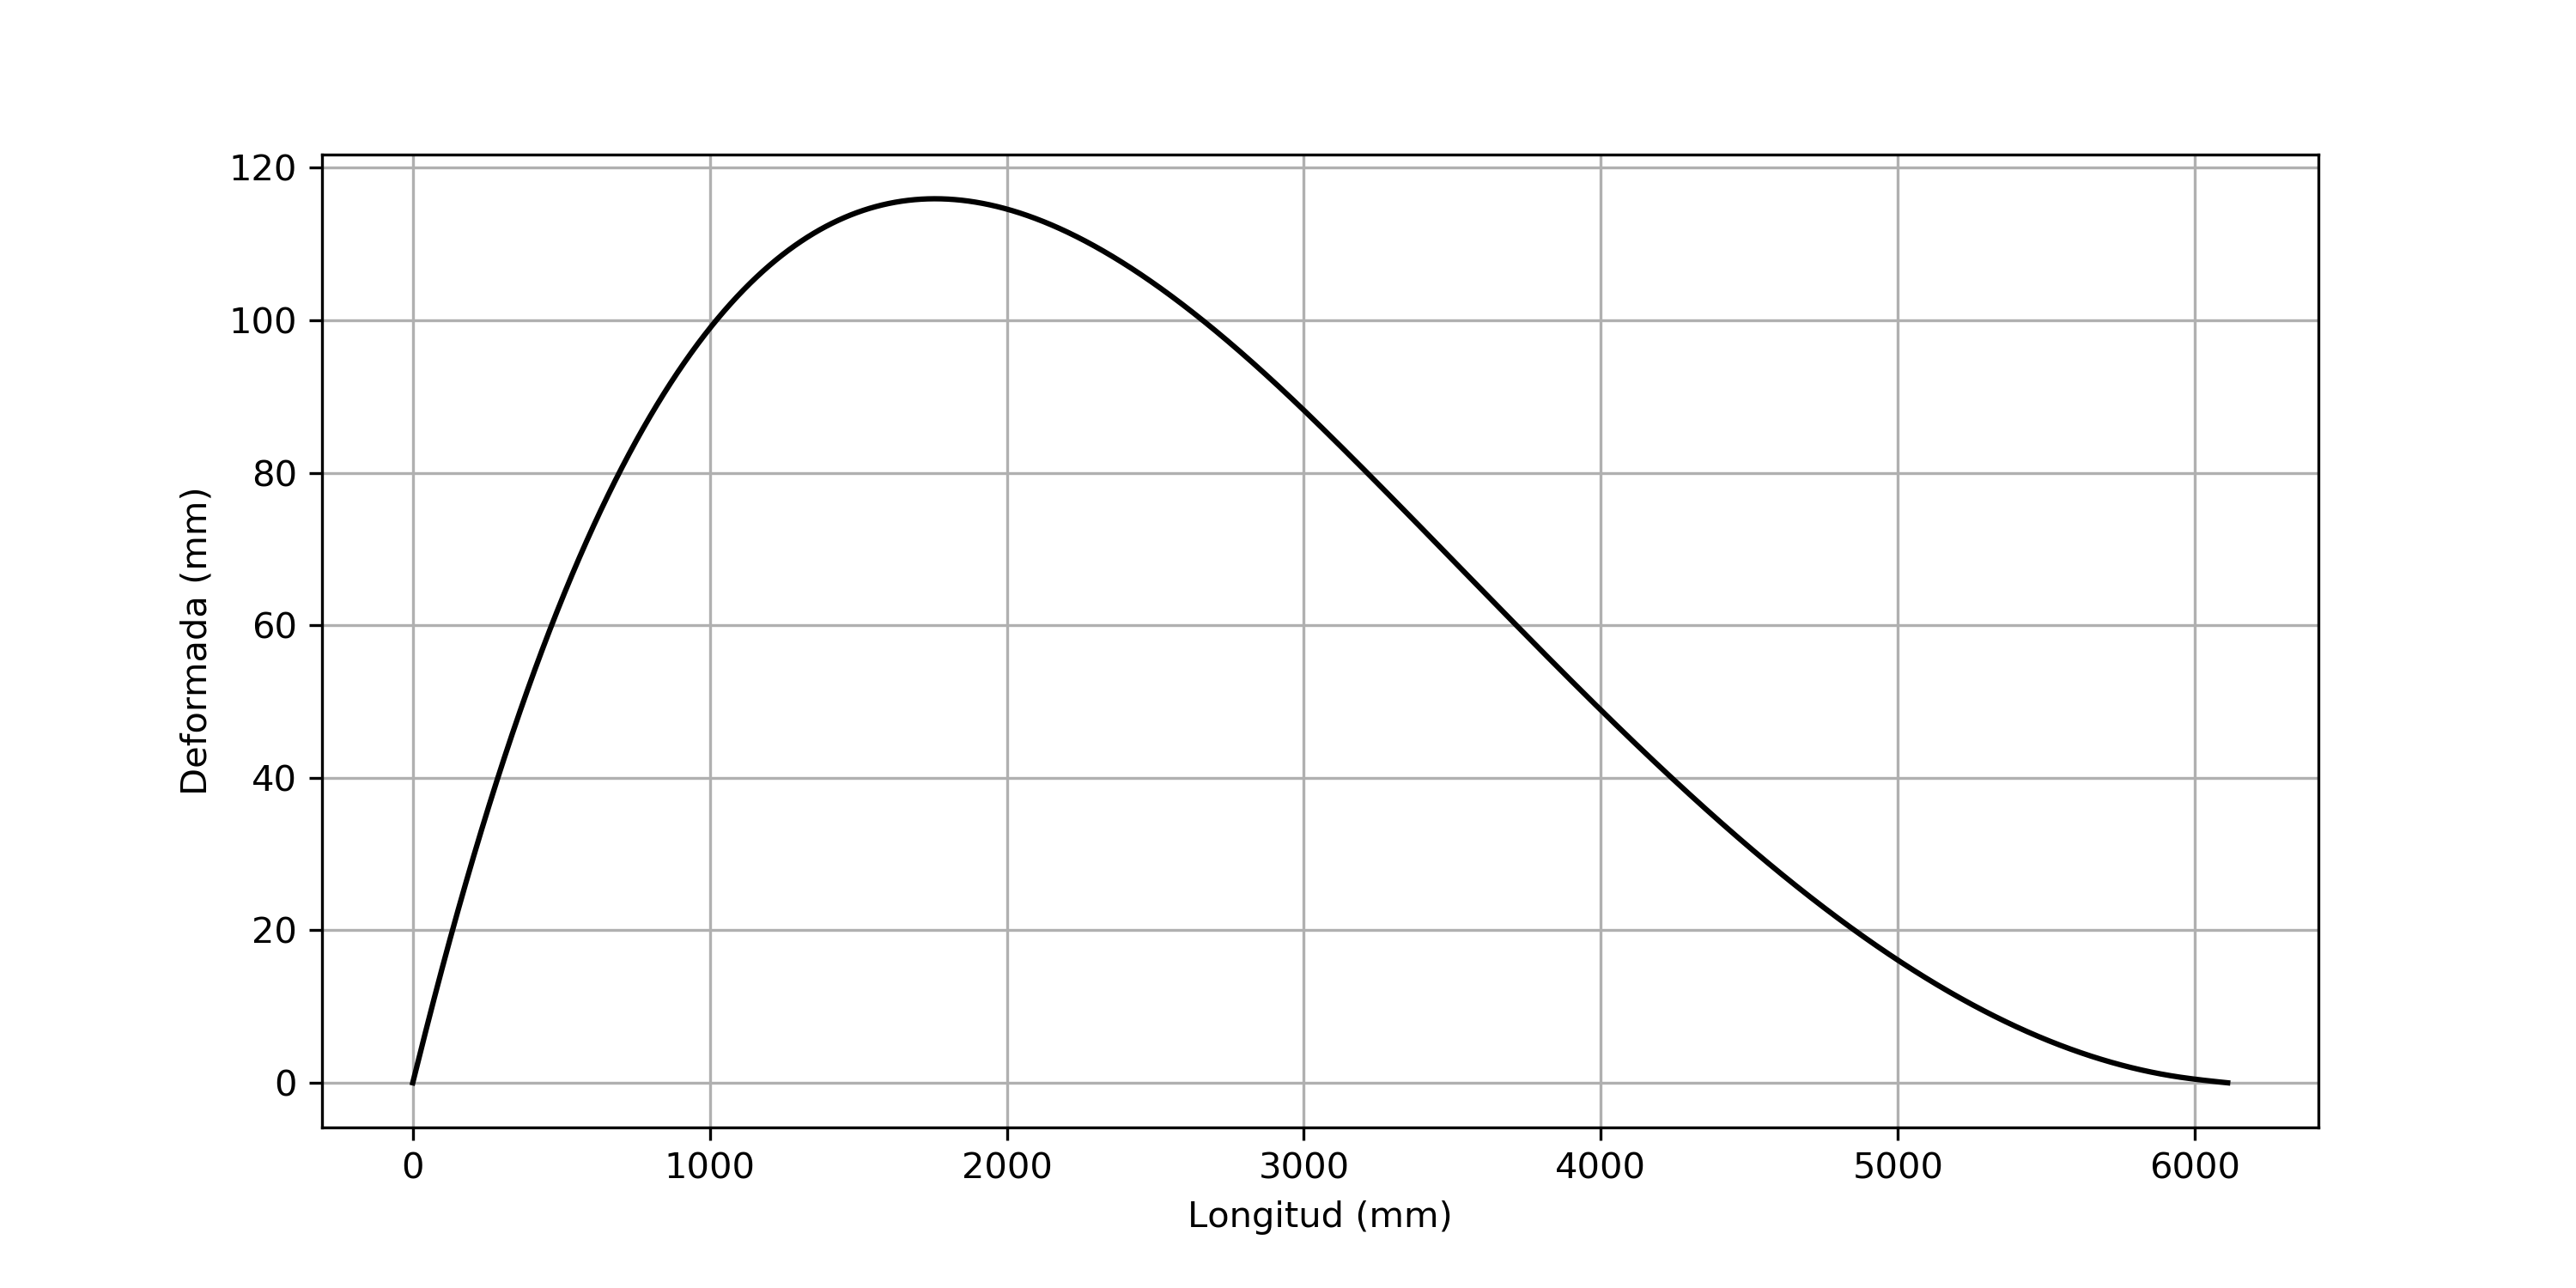
\includegraphics[scale=0.68]{defj2900.png}
\caption{$n = 2900$}
\end{figure}
El código utilizado se muestra a continuación:
\begin{pyglist}[language=python,caption={Cálculo de la flecha},style=tango]
for ka in range(1,30):
    n = ka
    R2 = 5*(2*n*n + 1135*n + 110780)/(n+155)
    R1 = 7340-60*n-R2
    v = []
    v.append(0)
    for x in range(1,310+2*n+1):
        aux = R1
        if x>10:
            aux = aux-(12-n)*(x-10)
        if x>130+2*n:
            aux = aux-(5000+10*n)
        if x>80:
            aux = aux + (12-n)*(x-80)
        if x>260+2*n:
            aux = aux+(50)*(x-(260+2*n)) + (5/12)*(x-(260+2*n))*(x-(260+2*n))
        if x>200+2*n:
            aux = aux-(5/12)*(x - (200+2*n))*(x - (200+2*n))
        if x>=310+2*n:
            aux = aux + R2
        v.append(aux)
    m = []
    for x in range(0,310+2*n+1):
        aux = R1*x
        if x>10:
            aux = aux-(12-n)*(x-10)*(x-10)/2
        if x>130+2*n:
            aux = aux-(5000+10*n)*(x-(130+2*n))
        if x>80:
            aux = aux + (12-n)*(x-80)*(x-80)/2
        if x>260+2*n:
            aux = aux+(25)*(x-(260+2*n))*(x-(260+2*n)) + (5/36)*(x-(260+2*n))**3
        if x > 130+2*n:
            aux = aux+(60000+200*n)
        if x>200+2*n:
            aux = aux-(5/36)*(x - (200+2*n))*(x - (200+2*n))*(x - (200+2*n))
        if x>=310+2*n:
            aux = aux + R2*(x-(310+2*n))
        m.append(aux)
    I = []
    for i in range(0,310+2*n+1):
        if i<10:
            I.append((math.pi*(40)**4)/64)
            continue
        if i<80:
            I.append((math.pi*(50)**4)/64)
            continue
        if i<200+2*n:
            I.append((math.pi*(((50+((i-80)*20/(120+2*n))))**4)/64))
            continue
        if i<260+2*n:
            I.append((math.pi*(70)**4)/64)
            continue
        if i<300+2*n:
            I.append((math.pi*(60)**4)/64)
            continue
        I.append((math.pi*(55)**4)/64)
    mi = []
    mi.append(0)
    for i in range(1,310+2*n+1):
        mi.append(m[i]/I[i] + mi[i-1])
    mii = []
    mii.append(0)
    for i in range(1,310+2*n+1):
        mii.append(mi[i]+mii[i-1])
    const = -mii[310+2*n]/(310+2*n)
    for i in range(0,310+2*n+1):
        mii[i] = (mii[i]+const*i)/E
    plt.figure(figsize=(10,5))
    plt.grid()
    plt.xlabel('Longitud (mm)')
    plt.ylabel('Deformada (mm)')
    plt.plot(mii,'-k')
\end{pyglist}
Observe que el valor de la $n$ va desde 1:30. Esto se puede modificar a gusto para observar otros valores de deformada. Así mismo, se calcula el cortante, el momento flector y el momento de inercia para cada posición longitudinal del eje. Para el cálculo se utiliza 310+2$n$ puntos.\\
Observamos que el algoritmo es muy óptimo. Pues la complejidad es de solo $O(n\cdot (310+2\cdot n)) \approx O(2n^{2})$. Es decir, en una computadora rutinaria se puede realizar alrededor de 1000 pruebas para distintos valores de $n$ y el resultado se mostraría en menos de un segundo. Todo el código fue implementado en Python\,3 y las gráficas hechas en matplotlib, para el cálculo simbólico se utilizó GNU Octave.\\
Adicionalmente, debido a la facilidad del código escrito, analizamos los valores de flecha máxima, su posición y el esfuerzo máximo para cada valor de $n$ hasta 600:
\begin{figure}[H]
\centering
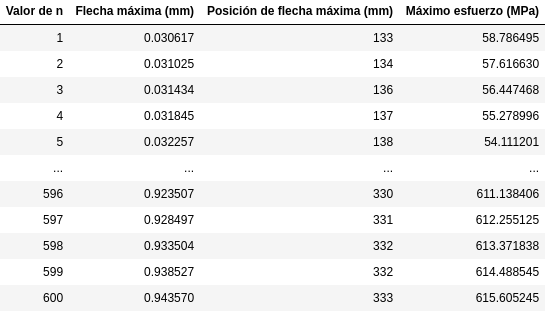
\includegraphics[scale=0.6]{allval.png}
\end{figure}
\begin{figure}[H]
\centering
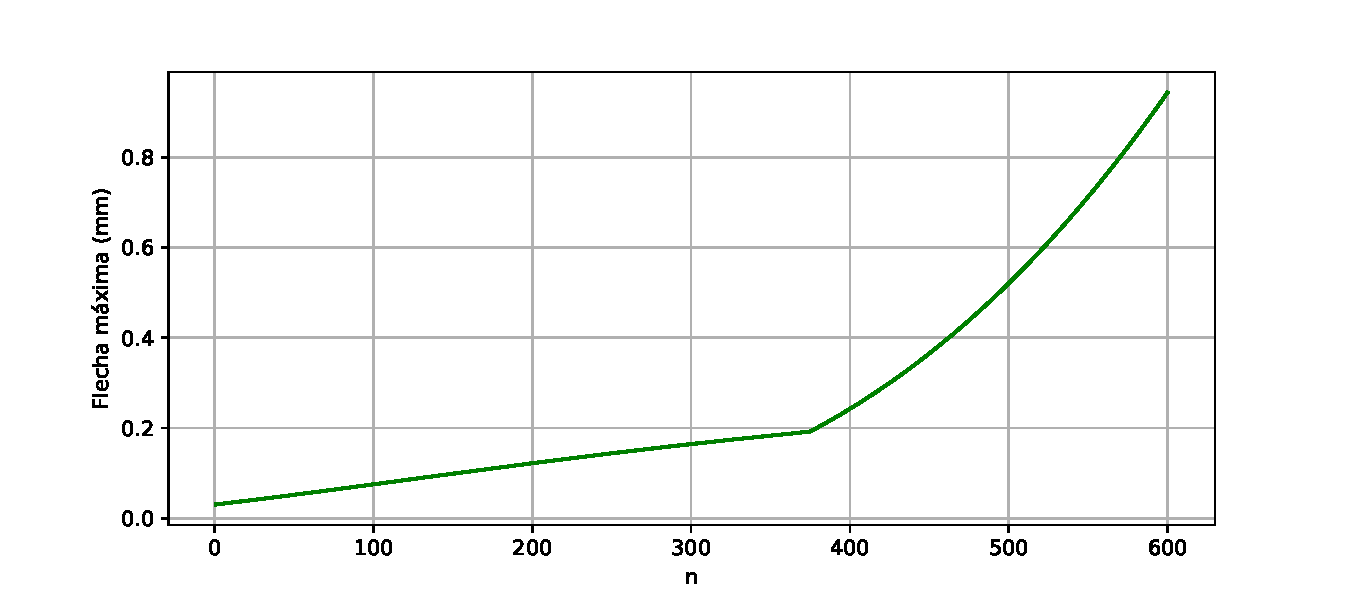
\includegraphics[scale=0.6]{maxflen.pdf}
\end{figure}
\begin{figure}[H]
\centering
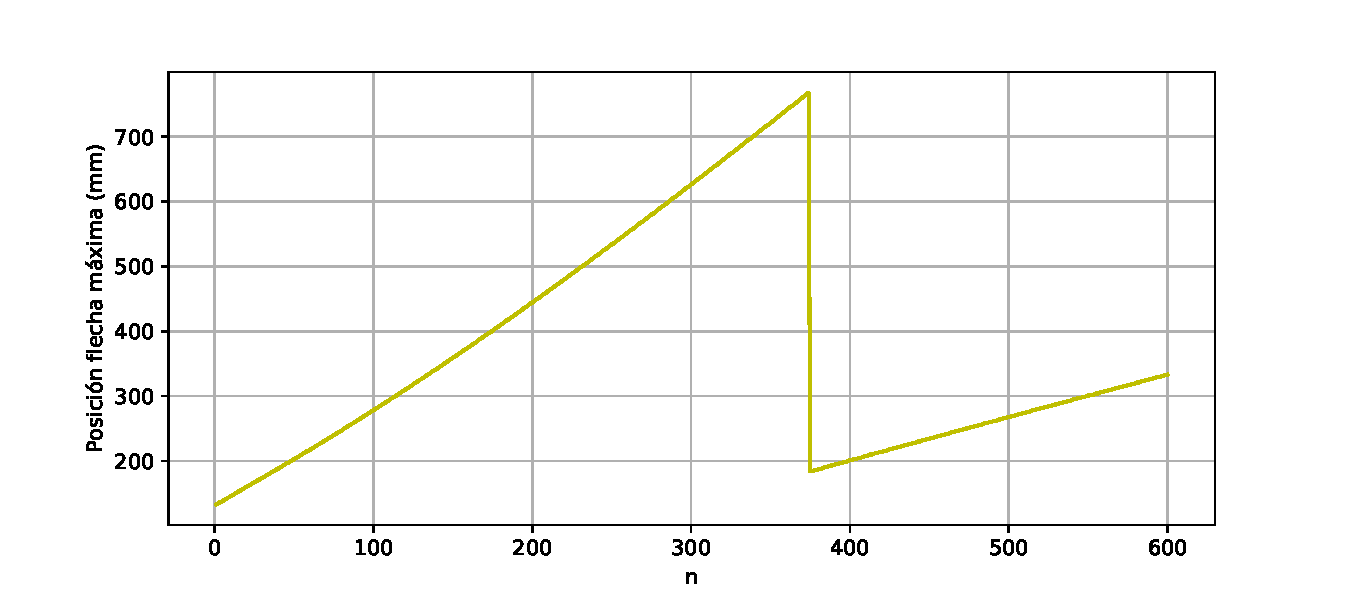
\includegraphics[scale=0.6]{posfn.pdf}
\end{figure}
\begin{figure}[H]
\centering
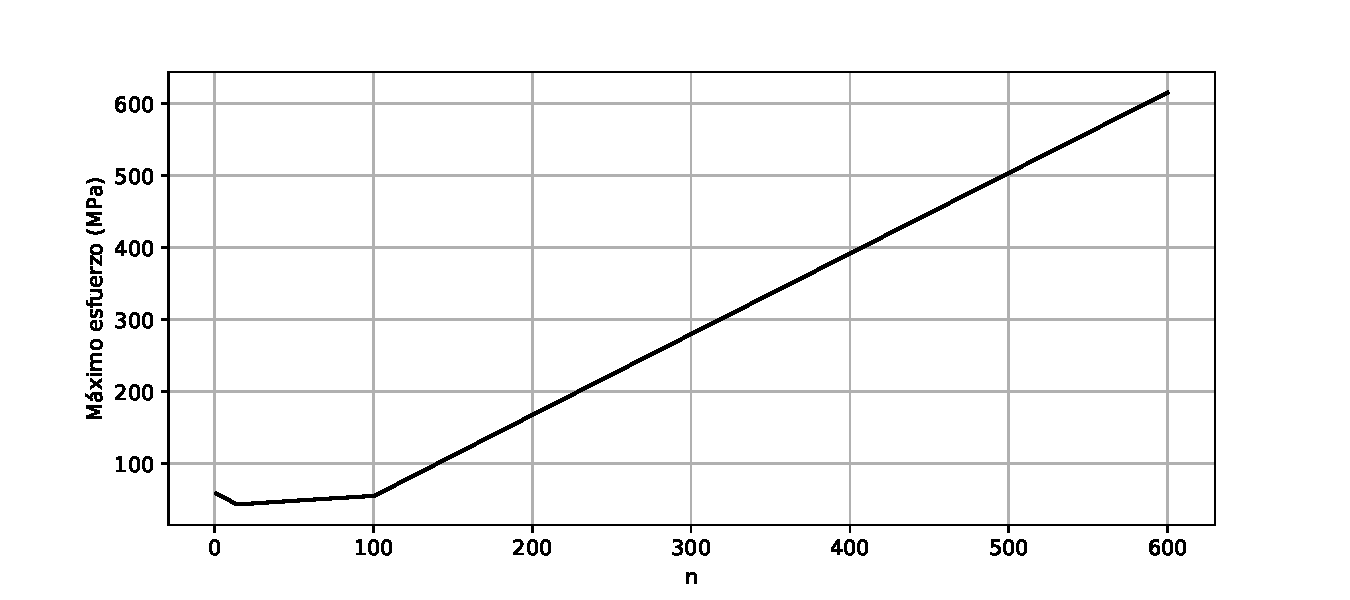
\includegraphics[scale=0.6]{allesf.pdf}
\end{figure}
Se observa un comportamiento lineal para los valores de la flecha máxima, cumpliéndose hasta cuando $n=375$, ahí es cuando la gráfica incrementa su pendiente y comienza a tener un crecimiento de flecha más acelerado.
\chapter{Conclusiones}
\begin{enumerate}
\item Se concluye que el eje no fallará, pues su deformada es muy pequeña comparada con su longitud y su esfuerzo es pequeño para producir la falla.
\item Se desprecia el peso del eje debido a que dicha fuerza es muy pequeña y solo haría más complicado los cálculos debido a que no es un eje simétrico.
\item Sin tanta pérdida de precisión, observamos que el procedimiento de aproximación de Riemann para el cálculo numérico de una integral nos ayuda para operar rápidamente la deformada del eje.
\item Con alrededor de 350 puntos sobre todo el eje podemos considerar que la aproximación tomada en la integral es lo suficientemente precisa para no cometer errores relativos superiores a 10$^{-5}$.
\item La velocidad de computación numérica es por mucho menos compleja que la simbólica en paquetes de software. Pues el cálculo exacto de $\iint M/I$ es demasiado complejo debido a las funciones singulares que aparecen; sin embargo por una suma acumulativa puede resolverse en una complejidad $O(n)$, es decir, se puede elevar la precisión hasta 100 veces más y seguir mostrando los resultados rápidamente.
\item Gracias a la facilidad del problema a ser parametrizado según $n$ es posible implementar un código sencillo en algún lenguaje de programación.
\item La ventaja de utilizar un lenguaje de programación para el problema es que podemos modificar un solo valor ($n$) para observar como varía el esfuerzo cortante, momento flector y deformada para todos esos valores de forma muy rápida; esto tomaría mucho tiempo en un un cálculo por elementos finitos que demanda un proceso de mallado y de diseño.
\item Con gran velocidad y precisión podemos notar observar que el eje no fallará por esfuerzo hasta valores muy grandes de $n$, el fallo ocurre pues por flexión, donde la flecha crece de manera rápida.
\item Si consideramos que el eje se trata de un acero A-36, comprobamos que para valores de $n$ mayor a 350 se llega al punto de fluencia. Mientras que para $n$ menores a 50 se tiene un factor de seguridad de 3.
\end{enumerate}
\end{document}